\chapter{Single-particle tracking}

XTrack is a 6D single particle symplectic tracking code used to compute the
trajectories of individual relativistic charged particles in circular
accelerators. It has been developed based on SixTrack.

The physical models are collected from the main references
\cite{ripken85,barber87,ripken95,heinemann95,barber96,beam_beam,rf_multipoles},
which contain more details of the derivation of the maps.


\section{Notation and reference frame}

The speed, momentum, energy, rest mass, charge of a particle are indicated
by $v$, $P$, $E$, $m$ and $q$, respectively.  These quantities are
related by the following equations:
\begin{align}
  v&=\beta c &
  E^2-P^2c^2&=m^2c^4 &
  E & = \gamma mc^2 &
  Pc & =\beta E
\end{align}
where $\beta$ and $\gamma$ are the relativistic factors.

In a curvilinear reference frame defined by a constant curvature $h_x$ in the
$\hat X, \hat Z$ plane and parameterized by $s$, the
position of the particle at a time $t$ can be written as:
\begin{align}
  \vec Q(t)= \vec r(s) + x \,\hat x(s) + y\, \hat y(s),
\end{align}
and therefore identified by the coordinates $s, x, y, t$ in the reference frame
defined by $\hat x(s)$ and $\hat y(s)$. In particle tracking, $s$ is normally
used as independent parameter and $t$ as a coordinate.

The electromagnetic fields {\bf E} and {\bf B} can be derived in a curvilinear
reference frame from the potentials $V(x,y,s,t)$ and $\mathbf{A}(x,y,s,t)$, where
\begin{align}
\mathbf{A}(x,y,s,t)=A_x(x,y,s,t) \hat x(s) + A_y(x,y,s,t) \hat y(s) + A_s(x,y,s,t) \hat z(s)
\end{align}
and for which:
\begin{align}
  \mathbf{E}  &= -\nabla V - \frac{\partial \mathbf{A}}{\partial t} 
               = -\partial_x V \hat x - \partial_y V \hat y -
  \frac{1}{1+h x}  \partial_s V \hat z - \partial_t \mathbf{A}\\
  \mathbf{B} &= \nabla\times\mathbf{A}  =
  \left(\partial_y A_s - \frac{\partial_s  A_y}{1+h x} \right) \hat x 
  +\left(\frac{\partial_s A_x-\partial_x (1+h x) A_s }{1+h x} \right)\hat y \\
  &+\quad \left(\partial_x A_y - \partial_y A_x \right) \hat z.
\end{align}
In this reference frame the canonical momenta are:
\begin{align}
  P_x&=m \gamma \dot x + q A_x, &
  P_y&=m \gamma \dot y + q A_y, &
  P_s&=m \gamma \dot s (1 + h x)^2 + q (1 + h x) A_s.
\end{align}
and the energy of a particle and the field is
\begin{align}
E=q\phi + c \sqrt{(mc)^2
              +\frac{(P_s- q A_s(1+hx))^2}{(1+hx)^2}
              +(P_x-q A_x)^2 + (P_y-q A_y)^2}.
\end{align}







\section{Hamiltonian and particle coordinates}

If $s(t)$ is monotonically increasing, it is possible to derive the equations
of motion using $s$ as the independent parameter, $(-t, E)$ as conjugate coordinates and $-P_s$ as Hamiltonian.

\begin{align}
  P_s&= (1+h x) \left( 
       \sqrt{ \frac{(E-q\phi)^2}{c^2} - (mc)^2
           - (P_x - q A_x)^2
           - (P_y - q A_y)^2}
       +q A_s
    \right)
\end{align}

Since in accelerators the orbits of the 
particles are often a perturbation of the reference trajectory followed by a
particle with rest mass $m_0$, charge $q_0$, speed $\beta_0 c$ and momentum
$P_0$, one could use the following derived quantities that usually assume small
values:
\begin{align}
p(x,y) &=
  \frac{m_0}{m}\frac{P(x,y)}{P_0}   &
\chi &=
  \frac{q}{q_0}\frac{m_0}{m} &
a(x,y,s) &=
  \frac{q_0}{P_0}  A(x,y,s)
\end{align}
Note that here $m$ is used to indicate the rest mass of particles of species
different from the reference particle (which has mass $m_0$) and not the relativistic mass.
Further rescaling the energy and charge density as
\begin{align}
  e(x,y,s) &=
  \frac{m_0}{m}\frac{E(x,y,s)}{P_0}   &
  \varphi(x,y,s) &=
  \frac{q_0}{P_0c}\phi(x,y,s) \,,
\end{align}
% This allows us to rewrite the Hamiltonian as:
% \begin{equation}\notag
%   - (1+h x) \, P_0\frac{m}{m_0}\left(
%       \sqrt{
%           \frac{\left(e - q\varphi\right)^2}{c^2} 
%             - \frac{1}{\beta_0^2\gamma_0^2}
%        - (p_x - \chi a_x)^2
%        - (p_y - \chi a_y)^2}
%        + \chi a_s
%     \right)
% \end{equation}
and as all canonical momenta scale with the same factor, we can define a new Hamiltonian
$\tilde{H}$ that still satisfies the same equations of motion:
\begin{align}\notag
  &\tilde{H}(x,y,-t, p_x, p_y, e) =
      \frac{m_0}{m}\frac{1}{P_0}H(x,y,-t, P_x, P_y, E) \\
  &\tilde{H}=
    - (1+h x) \left(
      \sqrt{ 
          \left(\frac{e}{c} - \chi\varphi\right)^2
            - \frac{1}{\beta_0^2\gamma_0^2}
           - (p_x - \chi a_x)^2
           - (p_y - \chi a_y)^2}
       + \chi a_s
    \right)
\end{align}

\subsection{Longitudinal coordinates}

Different sets of longitudinal coordinates can be used:
\begin{align}
\xi &= s \frac{\beta}{\beta_0} - \beta c t &
\tau &= \frac{s}{\beta_0} - ct &
\zeta &= s - \beta_0 ct \label{eq:coord1}&
\delta &=
  \frac{P \frac{m_0}{m} -P_0}{P_0} \\
\delta &=
  \frac{P \frac{m_0}{m} -P_0}{P_0} &
p_\tau &=
  \frac{1}{\beta_0} \frac{E \frac{m_0}{m} -E_0}{E_0} &
p_\zeta &=
  \frac{1}{\beta_0^2}\frac{E \frac{m_0}{m} -E_0}{E_0}&
\ell &= \beta c t
  \label{eq:coord2}
\end{align}
where variables in the same columns are canonically conjugate.

%As the position of the reference particle is given by
%$s=\beta_0ct_0$ we see that $\tau$ is the time advance of the tracked %particle w.r.t.\ 
%the reference particle:
%\begin{equation}
%  \tau = c\left(t_0-t\right) = c\Delta t
%\end{equation}
%This is the coordinate used by MAD-X. In Xsuite the pair $(\zeta, \delta)$ is used; note that
%these are not canonical as the canonical conjugates are the pairs $(\xi, \delta)$, $(\tau, p_\tau)$,
%and  $(\zeta, p_\zeta)$.

The different longitudinal variables can be easily related to each other:
\begin{align}
  &\xi= s \frac{\beta}{\beta_0} - \ell = 
      \beta\tau =
      \frac{\beta}{\beta_0}\zeta \\
  &p_\tau = \beta_0 p_\zeta\\
  &\delta= \sqrt{p_\tau^2 + 2 \frac{p_\tau}{\beta_0} +1} - 1
       =\beta p_\tau + \frac{\beta-\beta_0}{\beta_0}\\
  &\delta= \sqrt{\beta_0^2p_\zeta^2 + 2 p_\zeta +1} - 1
      =\beta\beta_0 p_\zeta + \frac{\beta-\beta_0}{\beta_0}\\
  &\gamma = \gamma_0 (1 + \beta_0 p_\tau)\\
  &\beta = \sqrt{1 - \frac{1 - \beta_0}{\left(1 + \beta_0 p_\tau\right)^2}}
\end{align}

For small energy deviations ($\delta \ll 1$, $p_\tau \ll 1$, $p_\zeta \ll 1$),
we can neglect the terms of order $\delta^2$, $p_\tau^2$, $p_\zeta^2$ and higher, hence
the following approximations hold:
\begin{align}
  &\delta \simeq \frac{p_\tau}{\beta_0} \\
  &\delta \simeq p_\zeta \\
  &\beta \simeq \beta_0 + (1 - \beta_0^2) p_\tau
\end{align}

\subsection{Hamiltonian with different coordinate choices}

The conjugate pairs can be generated by the following generating functions \footnote{
$F_2(-t , p_{\rm new}, s)$,\,
$e = \frac{\partial F_2}{\partial (-t)}$, \,
$q_{\rm new} = \frac{\partial F_2}{\partial p_{\rm new}}$,\,
$H_{\rm new} = H + \frac{\partial F_2}{\partial s}$
}

\begin{align}
F_2& = x p_x + y p_y + \left(\frac{s}{\beta_0}-ct\right)
                            \frac{1+\delta}{\beta} \\
F_2& = x p_x + y p_y + \left(\frac{s}{\beta_0}-ct\right)
                            \left(p_\tau + \frac{1}{\beta_0}\right) \\
F_2& = x p_x + y p_y + \left(\frac{s}{\beta_0}-ct\right)
                            \left(\beta_0 p_\zeta + \frac{1}{\beta_0}\right)
\end{align}

The Hamiltonians are then:

% \begin{align}
%  H_\delta   &= \frac{1+\delta}{\beta\beta_0} - \frac{m_0}{m}\frac{P_s}{P_0} &
%  H_\tau   &= \frac{p_\tau}{\beta_0} - \frac{m_0}{m}\frac{P_s}{P_0} &
%  H_\zeta &= p_\zeta - \frac{m_0}{m}\frac{P_s}{P_0}
% \end{align}

\begin{align*}
 H_\delta   &= \frac{1+\delta}{\beta\beta_0} - (1+h x) \left(
      \sqrt{ \left(\frac{1+\delta}{\beta}-\chi\varphi\right)^2
           - \frac{1}{\beta_0^2\gamma_0^2} 
           - (p_x - \chi a_x)^2
           - (p_y - \chi a_y)^2}
       + \chi a_s
    \right) \\
 H_\tau   &= \frac{p_\tau}{\beta_0} - (1+h x) \left(
      \sqrt{ \left(p_\tau+\frac{1}{\beta_0}-\chi\varphi\right)^2
           - \frac{1}{\beta_0^2\gamma_0^2}
           - (p_x - \chi a_x)^2
           - (p_y - \chi a_y)^2}
       + \chi a_s
    \right) \\
  H_\zeta &= p_\zeta - (1+h x) \left(
      \sqrt{ \left(\beta_0 p_\zeta+\frac{1}{\beta_0}-\chi\varphi\right)^2
           - \frac{1}{\beta_0^2\gamma_0^2}
           - (p_x - \chi a_x)^2
           - (p_y - \chi a_y)^2}
       + \chi a_s
    \right)
\end{align*}
% where 
% \begin{align}
% \delta &= \frac{P \frac{m_0}{m} -P_0}{P_0} &
% \chi &= \frac{q}{q_0}\frac{m_0}{m}.
% \end{align}
Note that things get complicated when using the pair $(\xi, \delta)$, as then the
Hamiltonian contains terms in $\beta$, which in turn depends on the energy.  In particular:
\begin{equation}
\frac{\partial \beta}{\partial \delta} =
    \beta\, \frac{1-\beta^2}{1+\delta}
\end{equation}

For this reason we prefer using $H_\tau$ when deriving the equations of motion. Note
that when $\varphi=0$, the Hamiltonian simplifies into:
\begin{equation}
H_\tau  =
\frac{p_\tau}{\beta_0} - (1+h x) \left(
      \sqrt{ \left(1+\delta\right)^2
           - (p_x - \chi a_x)^2
           - (p_y - \chi a_y)^2}
       + \chi a_s
    \right)
\end{equation}

The following identities are useful to derive the equations of motion:

\begin{align}
&\frac{\partial \delta}{\partial p_\tau} =
    \frac{p_\tau+1/\beta_0}{1+\delta} = \frac{1}{\beta} \\
&\frac{\partial}{\partial\delta}\left( 
    \frac{1+\delta}{\beta\beta_0}
  \right)=
    \frac{\beta}{\beta_0}
% \delta&=\sqrt{\beta_0^2 p_\zeta^2 + 2 p_\zeta +1} -1 &
% \frac{d \delta}{d p_\zeta}= \frac{\beta_0^2 p_\zeta+1}{1+\delta} = \frac{\beta_0}{\beta}
\end{align}

\section{Symplectic integrators}

\subsection{Hamiltonians of the implemented maps}
Xsuite provides maps for the following Hamiltonians

We call $\sqrt{...} = \sqrt{(1 + \delta)^2 - p_x^2 - p_y^2}$:

\begin{tabular}{llll}
\toprule
\textbf{Map} & \textbf{Parameters} & \textbf{Description} \\
\midrule
D   & l            & Drift exact   & 
$H_D = \frac{p_\tau}{\beta_0} - \sqrt{(1 + \delta)^2 - p_x^2 - p_y^2}$ \\
De  & l            & Drift expanded & 
$H_{De} = \frac{p_\tau}{\beta_0}-\frac{p_x^2+p_y^2}{2(1+\delta)}$\\
Dc  & l            & Correction drift exact & 
$H_{Dc} = H_D - H_{De}$\\
R   & h, l         & Curved drift& 
$H_R = \frac{p_\tau}{\beta_0} -(1 + hx) \left( \sqrt{...}\right)$\\
Br  & k0, l        & Rectangular bend & 
$H_{Br} = \frac{p_\tau}{\beta_0} -\sqrt{...} -b_1 x$
\\
B   & k0, l, h     & Exact Bend & 
$H_{B} = \frac{p_\tau}{\beta_0} -(1 + hx) \left( \sqrt{...} -k_0\left(x-\frac{hx^2}{2(1+hx)} \right) \right) $\\
Kh  & h, l            & Thin curvature kick & 
$H_{Kh} = -hx$\\
K0h & k0,l          & Weak focusing & 
$H_{K0h} = k_0 h \frac{x^2}{2}$\\
K0  & k0, l           & Dipole kick & 
$H_{K0} = k_0 x$\\
K1  & k1, l       & Quadrupole kick & 
$H_{K1} = k_1\frac{x^2 - y^2}{2}$\\
K1h & k1, h, l      & Quad correction & 
$H_{K1h} = k_1 h \frac{2 x^3 - 3 xy^2}{6}$\\
Kn  & kn, ks, l     & Multipole & 
$H_{Kn} = -\Re\left( \sum_{n=0}^N (k_n+i{\hat k}_n)\frac{(x+iy)^{n+1}}{(n+1)!}\right)$
\\
Knh & kn, ks, h  & Curved Multipoles & 
Not yet available\\
M   & k0, k1, l, h & 2nd order Hamiltonian & 
$H_{Kn} = \frac{p_\tau}{\beta_0} +  \frac{1}{2}\frac{p_x^2 + p_y^2}{(1 + \delta)} + (k_0 -h)x + \frac{k_0hx^2}{2} + k_1 \frac{x^2-y^2}{2} $
\\
S   & ks,l          & Solenoid & 
$H_{S} = \frac{p_\tau}{\beta_0} - \sqrt{(1 + \delta)^2 - \left(p_x-\frac{k_s}{2} y\right)^2 - \left(p_y+\frac{k_s}{2}\right)^2}$
\\
\bottomrule
\end{tabular}

\subsection{Magnet models}
The maps are combined to obtain the following models of magnetic elements:\\

\begin{tabular}{lll}
\toprule
\textbf{Model} & $h=0, ks=0$ & $h\neq0, ks=0$ \\
\midrule
rot-kick-rot & [D], [K0 K1 Kn] & [R], [K0 K0h K1 K1h Kn Knh] \\
bend-kick-bend & [Br],  [K1 Kn] & [B], [K1 K1h Kn Knh] \\
matrix-kick-matrix & [M], [Kn Dc] & [M], [K1h Kn Knh Dc] \\
drift-kick-drift-exact & [D], [K0 K1 Kn] & [D], [Kh K0 K0h K1 K1h Kn Knh] \\
drift-kick-drift-expanded & [De], [K0 K1 Kn] & [De], [Kh K0 K0h K1 K1h Kn Knh] \\
\bottomrule
\end{tabular}

\subsubsection{Map for the exact bend}

This map is adapted from \cite{forest99}.

\begin{align}
x(s) &= \frac{1}{hk_0} \left( h \sqrt{(1 + \delta)^2 - p_x(s)^2 - p_y^2} - \frac{dp_x(s)}{ds} - k_0 \chi \right) \\
p_x(s) &= p_x \cos(h s) + \left( \sqrt{(1 + \delta)^2 - p_x^2 - p_y^2} - k_0 \chi \left( \frac{1}{h} + x \right) \right) \sin(h s) \\
y(s) &= y + \frac{p_y s h}{k_0 \chi} + \frac{p_y}{k_0 \chi} \left( \sin^{-1} \left( \frac{p_x}{\sqrt{(1 + \delta)^2 - p_y^2}} \right) - \sin^{-1} \left( \frac{p_x(s)}{\sqrt{(1 + \delta)^2 - p_y^2}} \right) \right) \\
p_y(s) &= p_y \\
\delta(s) &= \delta \\
\zeta(s) &= \zeta -\frac{\beta_0}{\beta}
  \left[
  \frac{(1 + \delta) s h}{k_0 \chi} + \frac{(1 + \delta)}{k_0 \chi} \left( \sin^{-1} \left( \frac{p_x}{\sqrt{(1 + \delta)^2 - p_y^2}} \right) - \sin^{-1} \left( \frac{p_x(s)}{\sqrt{(1 + \delta)^2 - p_y^2}} \right) \right)
  \right]
\end{align}

\subsubsection{Map for the straight bend}

This map is adapted from \cite{forest99}.

\begin{align}
x(L) &= x + \frac{1}{k_0 \chi} \left( \sqrt{(1 + \delta)^2 - p_x(L)^2 - p_y^2} - \sqrt{(1 + \delta)^2 - p_x^2 - p_y^2} \right) \\
p_x(L) &= p_x - k_0 \chi L \\
y(L) &= y + \frac{p_y}{k_0 \chi} \left( \sin^{-1} \left( \frac{p_x}{\sqrt{(1 + \delta)^2 - p_y^2}} \right) - \sin^{-1} \left( \frac{p_x(L)}{\sqrt{(1 + \delta)^2 - p_y^2}} \right) \right) \\
p_y(L) &= p_y \\
\delta(L) &= \delta \\
\zeta(L) &= \zeta - \frac{\beta_0}{\beta}
\left[
\frac{1 + \delta}{k_0 \chi} \left( \sin^{-1} \left( \frac{p_x}{\sqrt{(1 + \delta)^2 - p_y^2}} \right) - \sin^{-1} \left( \frac{p_x(L)}{\sqrt{(1 + \delta)^2 - p_y^2}} \right) \right)
\right]
\end{align}


\section{Cavity time, energy errors and acceleration}

A cavity kick depends on:

\begin{equation}
\sin(2 \pi f T + \phi)
\end{equation}

where T is laboratory time.


For the most general case:

\begin{equation}
\sin(2 \pi f T + \phi) = \sin\left(2 \pi f \frac{s-\zeta}{\beta_0 c}  + \phi \right)
\end{equation}

Most codes drop the term $2 \pi f s / (\beta_0 c)$ that is

\begin{equation}
\sin(2 \pi f T + \phi) \to  \sin\left(- 2 \pi f \frac{\zeta}{\beta_0 c} + \phi\right)
\end{equation}

to make sure that a particle that is syncrhonous to the reference trajectory is in phase with the cavity.


\subsection{Implementing energy errors} 

One can define

\begin{equation}
\begin{aligned}
s &= s_0 + n (L_0-L) + n L\\
f_{\rm rev} &= \beta_0 c / L\\ 
f &= h f_{\rm rev}
\end{aligned}
\end{equation}

where $s_0$ is the path length at the cavity turn at 0, $L_0$ is the design circumference, $n$ is the turn number, $h$ is the harmonic number, L is the new path length with an energy error. Indeed one could write $L=L_0(1 +\eta \delta_s$) where $\eta$ is a constant property of the lattice.

Multiple cavities can have their own defined $L$.

Using these definitions, then


\begin{align}
\sin(2 \pi f T + \phi) =
&\sin\left(2 \pi h f_{\rm rev} \frac{s_0 + n(L_0-L) -\zeta}{\beta_0 c}  + \phi\right)\\
=&\sin\left(2 \pi h f_{\rm rev} \frac{n(L_0-L) -\zeta}{\beta_0 c}  + \phi'\right)
\end{align}


where $\phi'=\frac{2\pi h s_0}{L} + \phi$.


In MAD-X twiss and MAD8, indeed the longitudinal coordinates is directly $\zeta'=n(L_0-L) -\zeta$ and the term $n(L_0-L)$ is added smoothly in each thick element. This forces all the cavities to share the same $L$ or $f_{\rm rev}$.

In SixTrack or MAD-X track, one could simply define a turn dependent phase
\begin{equation}
\phi=\phi_0 + 2 \pi h f_{\rm rev} n(L_0-L)
\end{equation}
which is very general or in alternative add a special element that perform at each turn the following transformation:

\begin{equation}
\zeta_{\rm new}=(L_0-L) -\zeta_{\rm old} 
\end{equation}

\subsection{Acceleration}

Accelaration can be achieved by renormalized the relative variables using a new momentum reference. This has the side effect that the fields of the magnets (expressed in normalized strength) follow the energy ramp and that the cavity frequency (if expressed in terms of the harmonic number (NB we should perhaps change this in the Xtrack interface) is updated.

The re-normalization if done once at each turn is:

\begin{align}
p_{x,\rm new} &= p_{x,\rm old} \frac{P_{0,\rm old}}{P_{0,\rm new}} &
p_{y,\rm new} &= p_{y,\rm old} \frac{P_{0,\rm old}}{P_{0,\rm new}} \\
\delta_{\rm new}&= (\delta_{\rm old}+1) \frac{P_{0,\rm old}}{P_{0,\rm new}} -1 &
p_{\tau,\rm new} &= \frac{p_{\tau,\rm old}\, P_{0,\rm old}\,c + E_{0,\rm old} - E_{0,\rm new}}{P_{0,\rm new}c} \\
\zeta_{\rm new} &= s\beta_0 \left(\frac{1}{\beta_{0,\rm new}} -
\frac{1}{\beta_{0,\rm old}}\right) - \zeta_{\rm old} &
\tau_{\rm new} &= s\left(\frac{1}{\beta_{0,\rm new}} -  \frac{1}{\beta_{0,\rm old}}\right) - \tau_{\rm old} \\
\end{align}





\section{Beam elements}

\subsection{Drift}
A drift is a straight, field-free region ($h(x,y)=0$, $V=0$ and
$\mathbf{A}=0$).  The exact and expanded Hamiltonian for a drift space are
\begin{align}
  H_\tau =
    \frac{p_\tau}{\beta_0}  - \sqrt{(1+\delta)^2 - p_x^2 - p_y^2}
  &\approx
    \frac{p_\tau}{\beta_0} - \delta + \frac{1}{2}\frac{p_x^2+p_y^2}{1+\delta}.
\end{align}
% \begin{align}
%   H_\sigma = p_\sigma - \sqrt{(1+\delta)^2 - p_x^2 - p_y^2} &\approx
%   p_\sigma - \delta + \frac{1}{2}\frac{p_x^2+p_y^2}{1+\delta}.
% \end{align}

The map is given by solving the equations of motion:
\begin{align}
  \frac{\text{d} p_i}{\text{d}s} &= -\frac{\partial H}{\partial q_i} &
  \frac{\text{d} q_i}{\text{d}s} &=  \frac{\partial H}{\partial p_i} 
\end{align}
As there is no explicit dependency on the position coordinates in the Hamiltonian, the
momenta remain unchanged in a drift.

For the position coordinates, we get:
\begin{align}
  \left(x\right)' &=
        \frac{p_x}{p_z}
        \approx \frac{p_x}{1+\delta} \\
  \left(y\right)' &=
        \frac{p_y}{p_z}
        \approx \frac{p_y}{1+\delta} \\
  \left(\tau\right)' &=
        \frac{1}{\beta_0} - \frac{1}{\beta}\frac{1+\delta}{p_z}
        \approx \frac{1}{\beta_0} - \frac{1}{\beta} - \frac{1}{\beta}
                \frac{p_x^2 + p_y^2}{2} \\
  p_z &=
        \sqrt{(1+\delta)^2 - p_x^2 - p_y^2}
\end{align}



\subsubsection{Expanded Drift}

The map relative to the expanded Hamiltonian is then
\begin{align}
  x_p &= \frac{p_x}{1+\delta} & 
  y_p &= \frac{p_y}{1+\delta}  \\
  x & \leftarrow x + x_p l &
  y & \leftarrow y + y_p l
\end{align}
% \begin{align}
%   \tau & \leftarrow \tau +
%    \frac{l}{\beta_0} - \frac{l}{\beta} -
%     \frac{l}{\beta} \frac{x_p^2+y_p^2}{2}=
%     \tau+
%     l\left(\frac{\delta}{\beta_0}-\frac{p_t}{1+\delta} - \frac{x_p^2+y_p^2}{2\beta}\right)
% \end{align}
\begin{align}
  \zeta &
    \leftarrow \zeta+
    l\left(1- \frac{\beta_0}{\beta}\left(1 + \frac{x_p^2+y_p^2}{2}\right)\right)
\end{align}

\subsubsection{Exact Drift}

The map relative to the exact Hamiltonian is then
% \begin{align}
%   p_z&=\sqrt{(1+\delta)^2 - p_x^2 - p_y^2} \\
%   \frac{d p_z}{d p_t}&= \frac{p_t+1/\beta_0}{p_z} = \frac{1}{\beta_z}  \\
%   \frac{d p_z}{d p_\sigma}&= \frac{\beta_0^2 p_\sigma+1}{p_z} = \frac{\beta_0}{\beta_z}  
% \end{align}
\begin{align}
  x & \leftarrow x + \frac{p_x}{p_z} l  &
  y & \leftarrow y + \frac{p_x}{p_z} l
\end{align}
% \begin{align}
%   \tau & \leftarrow \tau + \frac{l}{\beta_0}
%   -\frac{l}{\beta_z}=
%   l\left(\frac{1}{\beta_0}-\frac{p_t+1/\beta_0}{p_z}\right)
% \end{align}
\begin{align}
  \zeta & \leftarrow \zeta + l\left(
          1-\frac{\beta_0}{\beta}\frac{1+\delta}{p_z}
          \right)
\end{align}




% \subsubsection{Polar Drift}
% It is possible to define a ``polar'' drift that has the effect of rotating the reference frame
% \cite{forest99} for instance in the $x$-$z$ plane

% \begin{align}
% p_x & \leftarrow   p_x \cos \theta + p_z \sin\theta &
% p_z & \leftarrow - p_x \sin \theta + p_z \cos\theta \\
% z   &= -x \sin \theta & x' &= p_x/p_z &  y' &= p_y/p_z \\
% x   & \leftarrow x \cos\theta - x' z  &
% y   & \leftarrow y - x' z  & \tau & \leftarrow \tau + z\frac{1}{\beta}\frac{1+\delta}{p_z} .
% \end{align}
% where $\theta$ is the angle bringing the new $\hat x$ towards the old $\hat z$.
% The map can be also generated by combining a rotation with a $-x
% \sin(\theta)$-length drift. In case of an $\hat x$ rotation the role of $x$ and $y$ are interchanged. 


\subsection{Thin dipole}

In a curvilinear reference system with a constant curvature $h$ in the
horizontal plane a uniform magnetic field can be derived by the vector potential:
\begin{align}
  A_x & = 0, & A_y & = 0, & A_s & = 
  - B_y \left(x-\frac{h x^2}{2 (1+h x)}\right).
\end{align}

With the following normalization $k_0=\frac{q_0}{p} B_y$ is the inverse of the bending 
radius of the reference particle.

The exact and expanded Hamiltonian for a horizontal bending magnet is (eq. 2.12 in
\cite{barber87})
\begin{align}
  H &= \frac{p_\tau}{\beta_0} 
       - (1+h x)\sqrt{(1+\delta)^2 -p_x^2 - p_y^2}
       + \chi k_0 \left( x + \frac{h x^2}{2} \right)  \\
    &\simeq   \frac{p_\tau}{\beta_0}
    + \frac{1}{2}\frac{p_x^2+p_y^2}{1+\delta}
  - (1+h x) (1+\delta) + \chi k_0 \left( x + \frac{h x^2}{2} \right)
\end{align}


The map for a thin dipole kick (horizontal or vertical) from the expanded Hamiltonian is 
(eq. 4.12 in \cite{heinemann95}):
\begin{align}
  p_x &\leftarrow p_x + (h_x l - \chi k_0 l)  + h_x l \delta - \chi k_0 l h_x x \\
  p_y &\leftarrow p_y - (h_y l - \chi \hat k_0 l) - h_y l \delta - \chi \hat k_0 l h_y y\\
  \tau &\leftarrow \tau - \frac{h_xx - h_yy}{\beta}  l.
\end{align}


%\subsubsection{mad thin dipole}
% see ttt = sqrt( one + two*track(6,jtrk)*beti + track(6,jtrk)*track(6,jtrk) ) 

%
%to be checked
%??? dipr 
%\begin{align}
%  p_x &\leftarrow p_x + (h_x l - \chi k_0 l)  + h_x l \delta - \chi k_0 l h_x x \\
%  p_y &\leftarrow p_y - (h_y l - \chi \hat k_0 l) - h_y l \delta  + \chi k_0 l h_y y\\
%  \tau &\leftarrow \tau - \frac{h_xx - h_yy}{\beta}  l.
%\end{align}

 %   ttt = sqrt( one + two*track(6,jtrk)*beti + track(6,jtrk)*track(6,jtrk) ) 
 %   track(2,jtrk) = track(2,jtrk) - (dbr + dxt(jtrk) - dipr * (ttt - one))
 %    track(4,jtrk) = track(4,jtrk) + (dbi + dyt(jtrk) - dipi * (ttt - one))
 %    track(5,jtrk) = track(5,jtrk) - &
 %         (dipr*track(1,jtrk) - dipi*track(3,jtrk)) *   &
 %         ((one + bet0*track(6,jtrk))/ttt) * bet0i






\subsection{Thin Multipole}

The effect of a thin multipole can be approximated by the following Hamiltonian

A longitudinally uniform static magnetic field can be described by the following equations
\begin{align}
    B_y+iB_x&=\sum_{n=1}     \frac{B_n+iA_n}{r_0^{n-1}} (x+iy)^{n-1} \\
            &=B_N \sum_{n=N} \frac{b_n+ia_n}{r_0^{n-1}} (x+iy)^{n-1}  .
\end{align}

%Usually multipole are expressed as relative to 
The kick $\Delta \vec P  = q_0 v_z \hat z \times (B_x \hat x + B_y \hat y)$ translates into
\begin{align}
   \Delta p_x - i \Delta p_y = -\frac{q_0}{P_0}\chi(B_y + i B_x) 
\end{align}


A thin multiple idealizes the effect of the field by taking the limit of the integration 
length going to zero while keeping constant the integrated strength. The Hamiltonian is:
\begin{align}
  H= \delta(s) \chi L \Re\left[\sum_{n=0} \frac{1}{(n+1)!}(k_n + i\hat k_n) (x+iy)^{n+1} \right].
\end{align}
where
\begin{align}
  k_n     &=  n!\frac{q_0}{p_0}  \frac{B_{n+1}}{r_0^n}  &
  \hat k_n&=  n!\frac{q_0}{p_0}  \frac{A_{n+1}}{r_0^n} .
\end{align}


The corresponding map is:
\begin{align}
  p_x &\leftarrow p_x - \chi L\cdot\Re\left[\sum_{n=0} \frac{1}{n!} (k_n + i\hat k_n) (x+iy)^n \right], \\
  p_y &\leftarrow p_y + \chi L\cdot\Im\left[\sum_{n=0} \frac{1}{n!} (k_n + i\hat k_n) (x+iy)^n \right],
\end{align}

In case a curvature $h$, the vector potential become:

\begin{align}
f(x,y)&=\int B_x(x,y) dy  \\
g(x,y)&=\int \partial x  B_x(x,y) dy \\
a_s(x,y)&=\frac{c_1}{1 + h x} + f(x,y) -
   \frac{\int_1^x (1 + h \tilde{x}) (g(\tilde{x},y)+\tilde{x}) +h f(x,y)  \, d\tilde{x}}{1+ h x}
\end{align}

\begin{align}
\frac{\int_1^x \left(-h \tilde{x} \left(g(x,y)\right)-\int \text{bx}^{(1,0)}(\tilde{x},y) \, dy-h \int \text{bx}(\tilde{x},y) \,
   dy-h \tilde{x} \text{by}(\tilde{x},y)-\text{by}(\tilde{x},y)\right) \, d\tilde{x}}{h x+1}
\end{align}



\subsection{Accelerating Cavity}

The approximated energy gain of a particle passing through an electric field of frequency $f=\frac{kc}{2\pi}$ for which:
\begin{align}
V \sin(\phi - k \tau) = \int_{-l/2}^{l/2} E_s(0,0,t,s)  {\rm \,d}s.
\end{align}

An equivalent vector potential can be derived and normalized as
\begin{align}
A_s& = - \frac{V}{\omega} \cos(\phi - k \tau ) & 
V_n&=  \frac{q_0}{P_0 c} V  & 
\end{align}
from which one can derive the following map
\begin{align}
p_\tau & \leftarrow p_\tau + \chi V_n \sin(\phi - k \tau + k \frac{s-s_0}{\beta_0}  ),
\end{align}
where the additional terms in the phase is added in case harmonic number is not exactly
integer and the phase is unlocked phase ). The new $\delta$ can be updated from the new $p_\tau$.



\subsection{RF-Multipole}

The RF-multipole generalizes the interaction of a particle with an electromagnetic field by assuming that

\begin{align}
\Delta E(x,y,\tau) &= q \int_{-L/2}^{L/2} E_z(x,y,t)  {\rm \,d}s \\
\Delta P_x(x,y,\tau) &= q \int_{-L/2}^{L/2} E_x(x,y,t) + \beta c B_y(x,y,t) {\rm \,d}s\\
\Delta P_y(x,y,\tau) &= q \int_{-L/2}^{L/2} E_y(x,y,t) - \beta c B_x(x,y,t) {\rm \,d}s.
\end{align}
are harmonic in $x,y$ and periodic in $\tau$ of frequency $f=\frac{k}{2\pi c}$ such that:

\begin{align}
a_s(x,y,\tau) 
&= \Re \left[ \sum_{n=1}^N
      \left(       k_n \cos(\phi_n -k \tau ) +
            i \hat k_n \cos(\hat \phi_n -k \tau)
      \right)    
      (x+i y )^n
     \right],
\end{align}

The map then follows:
\begin{align}
    \Delta p_x &= -\sum_{n=1}^N \frac{\chi}{n!} \Re\left[ (k_n C_n + i \hat k_n \hat C_n)(x+iy)^{(n-1)}\right], \\
    \Delta p_y &=  \sum_{n=1}^N \frac{\chi}{n!} \Im\left[ (k_n C_n + i \hat k_n \hat C_n)(x+iy)^{(n-1)}\right], \\
    \Delta p_\tau &= -\chi k \sum_{n=1}^N \Re\left[( k_n S_n + i k_n \hat S_n ) (x+iy)^n\right],
\end{align}
where
\begin{align}
     C_n&=\cos(\phi_n-\omega \Delta t) &
\hat C_n&=\cos(\hat \phi_n-\omega \Delta t) \\
     S_n&=\sin(\phi_n-\omega \Delta t) &
\hat S_n&=\sin(\hat \phi_n-\omega \Delta t) .
\end{align}


\subsection{Solenoid}

The derivation largely follows one by Forest~\cite{forest99}, while the final map can be verified to be the same as the one by Wolski~\cite{wolski2014beam}.

We can write the Hamiltonian for the solenoid as follows:
\begin{equation}
  H = p_\zeta -\sqrt{\left(1 + \delta \right)^2 - \left(p_x + \frac{b_z}{2}y\right)^2 - \left(p_y - \frac{b_z}{2}x\right)^2}
\end{equation}
where we have defined the normalized quantities $b_z = B_z\frac{q_0}{P_0}$, $a_x = A_x\frac{q_0}{P_0}$, $a_y = A_y\frac{q_0}{P_0}$.
This can be obtained knowing the general Hamiltonian
\begin{equation}
  H = p_\zeta -\sqrt{(1 + \delta)^2 - (p_x - a_x)^2 - (p_y - a_y)^2} - a_z,
\end{equation}
we can extract the magnetic field potential and convince ourselves that $H$ describes a magnetic field with only the longitudinal component equal to $B_z$, as expected of a solenoid:
\begin{equation}
  \mathbf{A} =
  \begin{bmatrix}
    A_x \\ A_y \\ A_z
  \end{bmatrix}
  = \begin{bmatrix}
    -\frac{B_z}{2}y\\
    \frac{B_z}{2}x\\
    0
  \end{bmatrix}
  %
  \implies
  %
  \mathbf{B} = \nabla \times \mathbf{A}
  = \begin{bmatrix}
    \frac{\partial A_z}{\partial y} - \frac{\partial A_y}{\partial z}\\
    \frac{\partial A_x}{\partial z} - \frac{\partial A_z}{\partial x}\\
    \frac{\partial A_y}{\partial x} - \frac{\partial A_x}{\partial y}\\
  \end{bmatrix}
  = \begin{bmatrix}
    0\\
    0\\
    B_z
  \end{bmatrix}.
\end{equation}

The Hamiltonian $H$ can be simplified, by applying the following transformation, which should be understood as the change of reference from the general coordinate system $\mathbf{X}$ to a new $\mathbf{X}_\text{new}$:
\[
  T := \begin{bmatrix}
  -\frac{1}{2} & 0 & 0 & \frac{1}{b_{z}} \\
  0 & 1 & \frac{1}{2} \, b_{z} & 0 \\
  -\frac{1}{2} & 0 & 0 & -\frac{1}{b_{z}} \\
  0 & 1 & -\frac{1}{2} \, b_{z} & 0
  \end{bmatrix}.
\]
In particular, note that if
\[
  \mathbf{X} =
  \begin{bmatrix}
    x \\ p_x \\ y \\ p_y
  \end{bmatrix}
  = T^{-1} \mathbf{X}_\text{new}
  = \begin{bmatrix}
    -x_\text{new} - y_\text{new} \\
    \frac{1}{2}(p_{x,\text{new}} + p_{y,\text{new}}) \\
    \frac{1}{b_z}(p_{x,\text{new}} - p_{y,\text{new}}) \\
    \frac{b_z}{2} (x_\text{new} - y_\text{new})
  \end{bmatrix},
\]
then we can rewrite $H$ in terms of $\mathbf{X}_\text{new}$ (dropping the `new' suffix, while keeping it in mind) as
\[
  K := -\sqrt{(1 + \delta)^2 - p_x^2 - b_z^2 x^2}.
\]
We can simplify $H$ even further, rewriting it in terms of the following action-angle variables:
\begin{equation}\label{eq:solenoid-x-px}
  x := \sqrt{\frac{2 J}{|b_z|}} \cos(\phi)
  \;\;\text{ and }\;\;
  p_x := \sqrt{2 |b_z| J} \sin(\phi).
\end{equation}
The new Hamiltonian with respect to $J$ is the following:
\begin{multline*}
  K = -\sqrt{(1 + \delta)^2 - p_x^2 - b_z^2 x^2} = \\
  %
  -\sqrt{(1 + \delta)^2 - \left(\sqrt{2 |b_z| J} \sin(\phi)\right)^2 - b_z^2 \sqrt{\frac{2 J}{|b_z|}} \cos(\phi)^2} = \\
  %
  -\sqrt{(1 + \delta)^2 - \left(\sqrt{2 |b_z| J} \sin(\phi)\right)^2 - \left(\sqrt{2 |b_z| J} \cos(\phi)\right)^2} = \\
  %
  -\sqrt{(1 + \delta)^2 - 2 |b_z| J}.
\end{multline*}
Then, using Hamilton's equations, we can solve for $\phi$:
\[
  \frac{d \phi}{d z} = \frac{\partial K}{\partial J} \implies \phi(z) = \phi(0) + z \frac{\partial K}{\partial J} = \phi(0) - z\frac{|b_z|}{K}.
\]
Let $\omega := -b_z / K$. Keeping in mind that we are still in the realm of $\mathbf{X}_\text{new}$, we can compute $x_\text{new}$ and $y_\text{new}$ substituting the above into (\ref{eq:solenoid-x-px}).
Note that we can drop the modulus on $b_z$ in both $\omega$ and the equations below, as $\cos$ is an even function, and while $\sin$ is an odd function and the signs of $\sin(\omega z)$ and $b_z$ will cancel out anyway.
\begin{multline*}
  x = \sqrt{\frac{2J}{|b_z|}} \cos\left(\phi(0) + \left(- z\frac{|b_z|}{K}\right)\right) = \\
    \sqrt{\frac{2J}{|b_z|}} \cos\phi(0) \cos(\omega z) - \frac{\sqrt{2J|b_z|}}{|b_z|} \sin\phi(0) \sin\left(- z\frac{|b_z|}{K}\right) = \\
    x_0 \cos(\omega z) - \frac{p_{x,0}}{b_z} \sin(\omega z)
\end{multline*}
\begin{multline*}
  p_x = \sqrt{2 |b_z| J} \sin\left(\phi(0) + \left(- z\frac{|b_z|}{K}\right)\right) = \\
    \sqrt{2 |b_z| J} \sin\phi(0) \cos(\omega z) + |b_z| \sqrt{\frac{2J}{|b_z|}} \cos\phi(0) \sin\left(- z\frac{|b_z|}{K}\right) = \\
    p_{x,0} \cos(\omega z) + b_z x_0 \sin(\omega z)
\end{multline*}
These equations give us the map for the solenoid in $\mathbf{X}_\text{new}$.
We can write this transformation in the form of a matrix
\[
R := \begin{bmatrix}
  \cos(\omega z) & -\frac{\sin(\omega z)}{b_z} & 0 & 0 \\
  b_z \sin(\omega z) & \cos(\omega z) & 0 & 0 \\
  0 & 0 & 1 & 0 \\
  0 & 0 & 0 & 1
\end{bmatrix},
\]
and therefore the whole solenoid map in $\mathbf{X}$ as follows (let $S := \sin(\omega z)$ and $C := \cos(\omega z)$):
\[
  M := T^{-1} R T = \begin{bmatrix}
    % 1st row
    \frac{C + 1}{2} &
    \frac{S}{b_z} &
    \frac{S}{2} &
    \frac{1 - C}{b_z} \\[6pt]
    % 2nd row
    -\frac{b_z S}{4} &
    \frac{C + 1}{2} &
    \frac{b_z (C - 1)}{4} &
    \frac{S}{2} \\[6pt]
    % 3rd row
    -\frac{S}{2} &
    \frac{C - 1}{b_z} &
    \frac{C + 1}{2} &
    \frac{S}{b_z} \\[6pt]
    % 4th row
    \frac{b_z (1 - C)}{4} &
    -\frac{S}{2} &
    -\frac{b_z S}{4} &
    \frac{C + 1}{2}
  \end{bmatrix}
\]

In the tracking procedure of Xtrack (and MAD-X) the map is implemented with respect to a different quantity \verb|sk|, which we will denote with $k$, and which represents half of magnetic field strength $b_z$: $k = \frac{b_z}{2}$.
Let $s := \sin(\frac{z k}{H}) = \sin(\frac{\omega z}{2})$ and $c := \cos(\frac{\omega z}{2})$; then we can rewrite $M$ using the trigonometric identities:
\begin{align*}
  \cos(2 \theta) = 2 \cos^2\theta - 1 = 1 - 2 \sin^2\theta &\implies c^2 = \frac{C + 1}{2} \text{ and } s^2 = \frac{1 - C}{2}, \\
  \sin(2 \theta) = 2 \cos\theta \sin\theta &\implies sc = \frac{S}{2},
\end{align*}
as the following transfer matrix
\[
  M = \begin{bmatrix}
    c^2 & \frac{cs}{k} & cs & \frac{s^2}{k} \\
    -kcs & c^2 & -ks^2 & cs \\
    -cs & -\frac{s^2}{k} & c^2 & \frac{cs}{k} \\
    ks^2 & -cs & -kcs & c^2
  \end{bmatrix},
\]
which, with relatively little effort, can be verified to correspond to the implementation of the tracking procedure.
We have the following map (note the change in $\zeta$ is analogous to the drift):

\begin{align*}
  x &\leftarrow {\left(x \cos\left(\theta\right) + y \sin\left(\theta\right)\right)} \cos\left(\theta\right) + \frac{2}{b_{z}} {\left(p_{x} \cos\left(\theta\right) + p_{y} \sin\left(\theta\right)\right)} \sin\left(\theta\right) \\
  p_x &\leftarrow -\frac{1}{2} \, {\left(x \cos\left(\theta\right) + y \sin\left(\theta\right)\right)} b_{z} \sin\left(\theta\right) + {\left(p_{x} \cos\left(\theta\right) + p_{y} \sin\left(\theta\right)\right)} \cos\left(\theta\right) \\
  y &\leftarrow {\left(y \cos\left(\theta\right) - x \sin\left(\theta\right)\right)} \cos\left(\theta\right) + \frac{2}{b_{z}} {\left(p_{y} \cos\left(\theta\right) - p_{x} \sin\left(\theta\right)\right)} \sin\left(\theta\right) \\
  p_y &\leftarrow -\frac{1}{2} \, {\left(y \cos\left(\theta\right) - x \sin\left(\theta\right)\right)} b_{z} \sin\left(\theta\right) + {\left(p_{y} \cos\left(\theta\right) - p_{x} \sin\left(\theta\right)\right)} \cos\left(\theta\right) \\
  \zeta &\leftarrow \zeta + L \left(1 - \frac{\beta_0}{\beta} \frac{1 + \delta}{p_z}\right),
\end{align*}
where $p_z :=  \sqrt{{\left(\delta + 1\right)}^2 - {\left(\frac{b_z}{2} x - p_{y}\right)}^{2} - {\left(\frac{b_{z}}{2} y + p_{x}\right)}^{2}}$, $\theta := \frac{b_{z} L}{2 p_z} $, and $L$ is the length of the thick solenoid.

\subsection{Tilted solenoid}

From solenoid frame (x'-z') to beam frame (x-z) we have the following transformation:
\begin{align}
x &= x' \cos\theta - z' \sin\theta \\
z &= x' \sin\theta + z' \cos\theta
\end{align}

The inverse transformation is:
\begin{align}
x' &= x \cos\theta + z \sin\theta \\
z' &= -x \sin\theta + z \cos\theta
\end{align}

We write the potential for solenoid with longitudinal field dependent on $z$:
\begin{align}
A_{x'} &= -\frac{B_A(z')}{2} \, y' \\
A_{y'} &= \frac{B_A(z')}{2} \, x' \\
A_{z'} &= 0
\end{align}

We compute the components in the beam frame:
\begin{align}
&A_x = \cos\theta \cdot A_{x'} - \sin\theta \cdot A_{z'} \\
&A_y = A_{y'} \\
&A_z = \sin\theta \cdot A_{x'} + \cos\theta \cdot A_{z'}
\end{align}

Replacing the coordinates $x', y', z'$ and using the notation abuse
$B_A(z) = B_A(z\,/\cos \theta)$, we obtain:
\begin{align}
&A_x = -\frac{B_A(z)}{2} \, y \cos\theta \\
&A_y = \frac{B_A(z)}{2} x \cos\theta + \frac{B_A(z)}{2} z \sin\theta \\
&A_z = -\frac{B_A(z)}{2} \, y \sin\theta
\end{align}

I do a change of gauge:
\begin{equation}
\mathbf{A}_\text{new} = \mathbf{A} + \nabla f
\end{equation}
with:
\begin{equation}
f = -\frac{B_A(z)}{2} \, y z \sin\theta
\end{equation}
obtaining:
\begin{align}
A_x &= -\frac{B_A(z)}{2} \, y \cos\theta \\
A_y &= \frac{B_A(z)}{2} \, x \cos\theta \\
A_z &= -B_A(z) \, y \sin\theta - \frac{1}{2} \frac{dB_A}{dz} \, z y \sin\theta
\end{align}

From this we compute the field $\mathbf{B} = \nabla \times \mathbf{A}$:
\begin{align}
B_x(x,y,z) &= -\frac{1}{2} \frac{dB_A}{dz} \, x \cos\theta - B_A(z) \sin\theta - \frac{1}{2} \frac{dB_A}{dz} \, z \sin\theta  \\
B_y(x,y,z) &= -\frac{1}{2} \frac{dB_A}{dz} \, y \cos\theta \\
B_z(x,y,z) &= B_A(z) \cos\theta
\end{align}

We call
\begin{align}
&\boxed{B_{x0}(z) = B_x(0,0,z) = -B_A(z) \sin\theta - \frac{1}{2} \frac{dB_A}{dz} \, z \sin\theta }\\
&\boxed{B_{z0}(z) = B_z(0,0,z) = B_A(z) \cos\theta}
\end{align}

We can use the above to express the field:
\begin{align}
&\boxed{B_x(x,y,z) = -\frac{1}{2} \frac{dB_{z0}}{dz} \, x  + B_{x0}(z)} \\
&\boxed{B_y(x,y,z) = -\frac{1}{2} \frac{dB_{z0}}{dz} \, y} \\
&\boxed{B_z(x,y,z) = B_{z0}(z)}
\end{align}
and to expres the vector potential:
\begin{align}
&\boxed{A_x = -\frac{B_{z0}(z)}{2} \, y}\\
&\boxed{A_y = \frac{B_{z0}(z)}{2} \, x}\\
&\boxed{A_z = B_{x0}(z) y}
\end{align}

\subsubsection{Generalization to arbitrary tilt and dipolar components}

If the tilt is not in the $x-z$ plane, and if additional dipolar components are present,
we can generalize the above obtaining the following vector potential:
\begin{align}
&\boxed{A_x = -\frac{B_{z0}(z)}{2} \, y}\\
&\boxed{A_y = \frac{B_{z0}(z)}{2} \, x}\\
&\boxed{A_z = B_{x0}(z) y - B_{y0}(z) x}
\end{align}
The corresponding magnetic field is:
\begin{align}
&\boxed{B_x(x,y,z) = -\frac{1}{2} \frac{dB_{z0}}{dz} \, x  + B_{x0}(z)} \\
&\boxed{B_y(x,y,z) = -\frac{1}{2} \frac{dB_{z0}}{dz} \, y + B_{y0}(z)} \\
&\boxed{B_z(x,y,z) = B_{z0}(z)}
\end{align}
%\section{Beam-Beam}
%
%The closed expression of an integrated kick experienced by a test particle of charge  $q=Z e$ due to a 2D uncoupled Gaussian charge distribution of total charge $q_b=N_b e$ defined by $\sigma_x, \sigma_y$ and located at $\Delta x, \Delta y$ from the test particle and moving at $v_z=\beta_b c$ from the test particle can be obtained through the use of complex the function \cite{bassetti-erskine}:
%
%\begin{align}
%w(z)=\exp({-z^2})\left(1+\frac{2i}{\sqrt{\pi}}\int_0^z \exp({\xi^2}) d\xi \right)=
%     \exp({-z^2}){\rm erfc}(-iz).
%\end{align}
%
%The kick can then be expressed as
%\begin{equation}
%\Delta p_y+i \Delta p_x= K_b \frac{\sqrt{\pi}}{r}
%\left( {\rm w}\left(\xi_1 \right)
%       -\exp\left( \xi_2^2-\xi_1^2 \right)
%         {\rm w}\left( \xi_2 \right)
%\right)
%\end{equation}
%or, when $\sigma_x=\sigma_y=\sigma$, with
%\begin{equation}
%\Delta p_y+i \Delta p_x= K_b \frac{i \Delta x+ \Delta y}{\Delta_x^2+\Delta y^2}
%\left( 1 - \exp\left(-\frac{\Delta x^2+\Delta y^2}{2\sigma^2}\right) \right)
%\end{equation}
%since $w(z) \leftarrow i / (\sqrt{\pi} z) $ for $z\leftarrow \infty$ with and where
%\begin{align}
%r&=\sqrt{2(\sigma_x^2 - \sigma_y^2)} &
%\xi_1&=\frac {\Delta x}r +i \frac {\Delta y}r &
%\xi_2= \frac{\Delta x\sigma_y}{r\sigma_x}+i \frac{\Delta y \sigma_x}{r\sigma_y}.
%\end{align}
%and where
%\begin{align}
%K_b 
%=\chi \frac{q_0 q_b  (1 -\beta \beta_b)}{2\pi \epsilon_0  P_0 c^2}
%=\frac{2 N_b Z r_0 (1 -\beta \beta_b)}{ \beta_0 \gamma_0} && 
%r_0=\frac{e^2}{4\pi\epsilon_0 m c^2},
%\end{align}
%
%In case the 2D distribution approximates the integrated effect of a longitudinal distribution (e.g. beam beam effect) the kick has to be scaled by a time of flight factor
%\begin{align}
%K_b^{BB}&=\frac{K_b}{\beta - \beta_b}, 
%\end{align}
%while in case the distribution is stationary of length L and charge density $\lambda$ such that $N_b=\lambda L$.
%\begin{align}
%K_b^{SC}&=\frac{K_b}{\beta}. 
%\end{align}
%
%In case the distribution is not longitudinally uniform and the potential of a slice of charge can be written as
%$q_b U(X,Y,Z,t)/(P_0 c)$ where $S=\frac{Z-\beta_0\tau}{2}$ is the location of the interaction point, 
%one can apply the so-called Synchro-Betatron mapping in the ultra-relativistic limit:
%\begin{align}
%x &\leftarrow x- S f_X & 
%y &\leftarrow y- S f_Y   \\
%p_x &\leftarrow p_x+  f_X=x'   &
%p_y &\leftarrow p_y+  f_Y=y' 
%\end{align} 
%\begin{align}
%p_t & \leftarrow p_t  + \frac{1}{2}
%   \left( f_Z 
%        + f_X \frac{p_x +x'}{2} 
%        + f_Y \frac{p_y +y'}{2} \right)
%\end{align} with $f_{X,Y,Z}=- n \partial_{X,Y,Z} U(X=x+S p_x,Y=y+S p_y,Z=Z,t=\tau)$.
%
%In the non-relativistic limit:
%\begin{align}
%f_{X,Y} &= - q_b \frac{1 -\beta \beta_b}{\beta - \beta_b} \partial_{X,Y} U&
%f_Z &= - q_b \frac{1}{\beta - \beta_b} \partial_Z U \\
%S&=\beta_0 \frac{Z/\beta-\tau}{\beta - \beta_b}&
%p_t & \leftarrow p_t  + \frac{\beta_0}{\beta-\beta_b}\left(\ldots\right)
%\end{align}.

\subsection{AC-dipole}
The excitation amplitude of the AC-dipole is denoted by $A$ [Tm], the excitation frequency by $q_d$ [$2\pi$] and the phase of the excitation by $\phi$. The map
presented here is for a purely horizontal dipole, the map for a vertical dipole is obtained by replacing $p_x\to p_y$.

The effect of the AC-dipole is split into four stages. The turn number is denoted by $n$.
\begin{enumerate}
  \item A number of free turns $n_{\text{free}}$, in which the AC-dipole has no effect on the motion.
  \item Ramp-up of the voltage from $0$ to the excitation amplitude $A$ for $n_{\text{ramp-up}}$ turns.
        \begin{align*}
            n' &= \frac{n-n_{\text{free}}}{n_{\text{ramp-up}}} \\
            p_x &\to p_x + n' \cdot \frac{A}{pc} \cdot(1+\delta) \sin\left(2\pi q_d\cdot(n-n_{\text{free}})+\phi\right)
        \end{align*}
  \item Constant excitation amplitude for $n_{\text{flat}}$ turns.
        \begin{align*}
            p_x &\to p_x + \frac{A}{pc}\cdot(1+\delta)\sin\left(2\pi q_d\cdot(n-n_{\text{free}})+\phi\right)
        \end{align*}
  \item Ramp-down of the voltage from the excitation amplitude $A$ to $0$ for $n_{\text{ramp-down}}$ turns.
        \begin{align*}
            n' &= \frac{n-n_{\text{free}}-n_{\text{ramp-up}}-n_{\text{flat}}-n_{\text{ramp-down}}}{n_{\text{ramp-down}}} \\
            p_x &\to p_x + n' \cdot \frac{A}{p} \cdot(1+\delta) \sin\left(2\pi q_d\cdot(n-n_{\text{free}})+\phi\right)
        \end{align*}
\end{enumerate}

\subsection{Wire}
For each part we define $p_z=\sqrt{(1+\delta)^2-x'^2-y'^2}$, using the current values for $x'$ and $y'$.

Step 1. Initial backwards drift of length $L=\frac{embl}{2}$.
\begin{align*}
	x &\to x - L\cdot\frac{x'}{p_z} \\
    y &\to y - L\cdot\frac{y'}{p_z}
\end{align*}

Step 2.
\begin{align*}
	y &\to y - \frac{x\cdot\sin(t_x)}{
    \cos\left(\arctan\left(\frac{x'}{p_z}\right)-t_x\right)}\cdot
    \frac{y'}{\sqrt{(1+\delta)^2-y'^2}} \\
    x &\to x\cdot\left[\cos(t_x)-\sin(t_x)\cdot\tan\left(
    \arctan\left(\frac{x'}{p_z}\right)-t_x\right)\right] \\
    x' &\to \sqrt{(1+\delta)^2-y'^2}\cdot\sin\left(
    \arctan\left(\frac{x'}{p_z}\right)-t_x\right) \\
    x &\to x- \frac{y\cdot\sin(t_y)}{\cos\left(\arctan\left(\frac{y'}{p_z}\right)
    -t_y\right)} \cdot\frac{x'}{\sqrt{(1+\delta)^2-x'^2}} \\
    y &\to y \left[ \cos(t_y) - \sin(t_y)\cdot\tan\left(
    \arctan\left(\frac{y'}{p_z}\right)-t_y\right) \right] \\
    y' &\to \sqrt{(1+\delta)^2-x'^2}\sin\left(\arctan\left(
    \frac{y'}{p_z}\right)-t_y\right)
\end{align*}

Step 3. Drift part of length $L=lin$.
\begin{align*}
    x &\to x + L \cdot \frac{x'}{p_z} \\
    y &\to y + L \cdot \frac{y'}{p_z}
\end{align*}

Step 4. Here $x_i=x-r_x$ and $y=y-r_y$.
\begin{align*}
    x' &\to x' - \frac{\frac{cur\cdot10^{-7}}{chi}\cdot x_i}{x_i^2+y_i^2}
    \left[\sqrt{(lin+l)^2+x_i^2+y_i^2}-\sqrt{(lin-l)^2+x_i^2+y_i^2} \right] \\
    y' &\to y' - \frac{\frac{cur\cdot10^{-7}}{chi}\cdot y_i}{x_i^2+y_i^2}
    \left[\sqrt{(lin+l)^2+x_i^2+y_i^2}-\sqrt{(lin-l)^2+x_i^2+y_i^2} \right]
\end{align*}

Step 5. Drift of length $L=leff-lin$.
\begin{align*}
    x &\to x + L \frac{x'}{p_z} \\
    y &\to y + L \frac{y'}{p_z}
\end{align*}

Step 6.
\begin{align*}
	x &\to x - \frac{y\cdot\sin(-t_y)}{
    \cos\left(\arctan\left(\frac{y'}{p_z}\right)+t_y\right)}\cdot
    \frac{x'}{\sqrt{(1+\delta)^2-x'^2}} \\
    y &\to y\cdot\left[\cos(-t_y)-\sin(-t_y)\cdot\tan\left(
    \arctan\left(\frac{y'}{p_z}\right)+t_y\right)\right] \\
    y' &\to \sqrt{(1+\delta)^2-x'^2}\cdot\sin\left(
    \arctan\left(\frac{y'}{p_z}\right)+t_y\right) \\
    y &\to y- \frac{x\cdot\sin(-t_x)}{\cos\left(\arctan\left(\frac{x'}{p_z}\right)
    +t_x\right)} \cdot\frac{y'}{\sqrt{(1+\delta)^2-y'^2}} \\
    x &\to x \left[ \cos(-t_x) - \sin(-t_x)\cdot\tan\left(
    \arctan\left(\frac{x'}{p_z}\right)+t_x\right) \right] \\
    x' &\to \sqrt{(1+\delta)^2-y'^2}\cdot\sin\left(\arctan\left(
    \frac{x'}{p_z}\right)+t_x\right)
\end{align*}

Step 7. Shift.
\begin{align*}
    x &\to x + embl\cdot \tan(t_x) \\
    y &\to y + embl\cdot\frac{\tan(t_y)}{\cos(t_x)}
\end{align*}

Step 8. Negative drift of length $L=\frac{embl}{2}$.
\begin{align*}
    x &\to x - L\cdot \frac{x'}{p_z} \\
    y &\to y - L\cdot \frac{y'}{p_z}
\end{align*}


\subsection{Electron Lens}
\label{elense}
\subsubsection{Hollow electron lens - uniform annular profile}
For a uniform distribution of the electron beam between $R_1$ and $R_2$, the radial kick can be described by a shape function $f(r)$ and a maximum kick strength $\theta_{\rm max}$:
\begin{equation}
\theta(r)=\frac{f(r)}{(r/R_2)}\cdot \theta_{\rm max}
\end{equation}
with $r=\sqrt{x^2+y^2}$ and $\theta_{\rm max}$ independent of $r$. The shape function $f(r)$ is defined as
\begin{equation}
f(r) = \frac{I(r)}{I_T}=\frac{2\pi}{I_T}\int_{0}^r r\rho(r) dr
\end{equation}
where $I_T$ is the total electron beam current, $I(r)$ is the current enclosed in a radius $r$ and $\rho(r)$ is the electron beam density distribution.

For a uniform profile one then obtains:
\begin{equation}
\begin{cases} 0 &,\quad r< R_1\\
\frac{r^2-R_1^2}{R_2^2-R_1^2} &,\quad R_1 \leq r < R_2\\
1 &,\quad R_2 \leq r
\end{cases}
\end{equation}
and
\begin{equation}
\theta_{\rm max} = \theta(R_2) = \frac{2LI_T(1\pm\beta_e\beta_p)}{4\pi\epsilon_0  \left(B\rho\right)_p\beta_e\beta_p c^2}\cdot\frac{1}{R_2}
\end{equation}
where $L$ is the length of the e-lens, $I_T$ the total electron beam current, $\beta_{e/p}$ the relativistic $\beta$ of electron/proton beam, $B\rho$ the magnetic rigidity, $c$ the speed of light and $\epsilon_0$ the vacuum permittivity. The $\pm$-sign represents the two cases of the electron beam traveling in the direction of the proton beam ($+$) or in the opposite direction ($-$). For hollow electron beam collimation, electron and proton beam travel in the same direction.

The kick in $(x',y')$ can then be expressed as (note $\frac{x}{r}=\cos(\phi),\frac{y}{r}=\sin(\phi)$):
\begin{align}
x'&=x'-\theta_{\rm max}\cdot\frac{r_2}{r^2}\cdot f(r)\cdot x\\
y'&=y'-\theta_{\rm max}\cdot\frac{r_2}{r^2}\cdot f(r)\cdot y
\end{align}
If the electron lens is offset by $(x_{\rm offset},y_{\rm offset})$, the coordinates $(x,y)$ are simply transfered to:
\begin{align}
\tilde x&=x+x_{\rm offset}\\
\tilde y&=y+y_{\rm offset}\\
\tilde r&=\sqrt{\tilde x^2+\tilde y^2}
\end{align}
and the kick is then given by:
\begin{align}
x'&=x'-\theta_{\rm max}\cdot\frac{r_2}{\tilde r^2}\cdot f(\tilde r)\cdot \tilde x\\
y'&=y'-\theta_{\rm max}\cdot\frac{r_2}{\tilde r^2}\cdot f(\tilde r)\cdot \tilde y
\end{align}

\subsection{Electron Cooler}

The Parkhomchuk electron cooler in Xsuite applies a kick to the circulating ion based on the following equation:
%
\begin{equation}
\vec{F} = -\frac{n_e q^2 e^4}{4 \pi^2 \epsilon_0^2 m_e} \cdot \frac{d\vec{V}}{V^3_\text{tot}} \ln\left(\frac{\rho_{\max} + \rho_{\min} + \rho_{\mathrm{L}}}{\rho_{\min} + \rho_{\mathrm{L}}}\right),
\label{eq: parkhomchuk}
\end{equation}
%
Where \( \vec{F} \) is the friction force acting on the circulating particle, \( n_{e} \) is the electron density (per unit volume), \( q \) is the charge of the circulating particle, \( e \) is the elementary charge, \( m_e \) is the electron mass, \( d\vec{V} \) is the velocity difference between the circulating particle and the local electron velocity. \( \rho_{\max} \) and \( \rho_{\min} \) are the maximum and minimum impact parameters, respectively, and \( \rho_{\mathrm{L}} \) is Larmor radius of the electrons (also known as the radius of gyration). $V_{\text{tot}}$ represents the total velocity difference between the electrons and ion, which is given by:
%
\begin{equation}
V_{\text{tot}} = \sqrt{dV^2 + \Delta_{\parallel}^2 + \Delta_\text{magnet}^2}, 
\label{eq: total_velocity_difference}
\end{equation}
%
Where \( dV^2 = dV_x^2 + dV_y^2 + dV_z^2 \) is the squared norm of the relative velocity difference between the ion and electron. To prevent the cooling force from diverging as \( dV \to 0 \), regularization terms are added. The most logical approach is to add the temperatures as regularization terms because they provide the RMS velocity difference when \( dV = 0 \). This is why \( \Delta_{\parallel} \) the longitudinal electron velocity spread associated with their temperature is added to Equation~\eqref{eq: total_velocity_difference}. Lastly, \( \Delta_\text{magnet} \) is the additional velocity spread induced by imperfections in the magnetic field of the electron cooler solenoid, which is given by:
\begin{equation}
\Delta_\text{magnet} = c \gamma \frac{B_\perp}{B_\parallel}
\end{equation}
Where \( \frac{B_\perp}{B_\parallel} \) is the ratio of the transverse component of the magnetic field with respect to the longitudinal component. The transverse temperature is not included in Eqaution~\eqref{eq: total_velocity_difference} because it is suppressed due to the gyration motion of the electrons in the magnetic field. The transverse temperature indirectly plays a role in the Parkhomchuk model via the Larmor radius \( \rho_\text{L} \), which is given by:
%
\begin{equation}
\rho_{\text{L}} = \frac{m_e \Delta_{\perp}}{e B}
\label{eq: larmor_radius}
\end{equation}
%
Where \(\Delta_{\perp}\) is the transverse velocity due to the transverse electron temperature and \(B\) is the magnetic field. 
%
The minimum impact parameter \( \rho_{\text{min}} \) is given by:
\begin{equation}
\rho_{\text{min}} = \frac{Z e^2}{4 \pi \varepsilon_0 m_e \vec{V}^2}
\label{eq: minimum_impact_parameter}
\end{equation}
%
The maximum impact parameter determines the maximum length scale at which a Coulomb interaction takes place, which can be limited by various physical effects, such as the Debye length and it is given by:
%
\begin{equation}
    \rho_d = \frac{\Delta_{\parallel}}{\omega_p},
\end{equation}
%
Where the longitudinal velocity spread of the electrons \( \Delta_{\parallel}  \) is given by:
%
\begin{equation}
   \Delta_{\parallel} = \sqrt{\frac{k_B T}{m_e}}
\end{equation}
%
The plasma frequency \( \omega_\text{p} \)  represents the natural oscillation frequency of the electron due to a perturbation in its charge distribution, which is given by:
%
\begin{equation}
\omega_\text{p} = \sqrt{\frac{n_e e^2}{m_e \epsilon_0}}.
\end{equation}
%
The Debye radius is not the only limitation for the maximum interaction length. In the case where the velocity difference between the ion and electron \( d\vec{V} \) is sufficiently larger than the velocity spread of the electron \( \Delta_{\parallel} \), then the maximum shielding radius \( \rho_\text{s} \) is given by:
%
\begin{equation}
    \rho_\text{s} = \frac{d\vec{V}}{\omega_p}.
\end{equation}
%
In principle, it is necessary to compute both \( \rho_\text{d} \) and \( \rho_\text{s} \) and compare them to see which one is the bottleneck and use that as the maximum impact parameter, which is given by:
%
\[
\rho_\text{max} = \text{min}(\rho_\text{d},\rho_\text{s})
\]
%
However, in the code, the two shielding impact parameters are merged into a single effective impact parameter, given by:
%
\begin{equation}
\rho_\text{shield} = \frac{V_{\text{tot}}}{\omega_p}.
\label{eq: rho_shield_combined}
\end{equation}
%
Here, \( V_{\text{tot}} \) is the total velocity difference between the electron and ion from Equation~\ref{eq: total_velocity_difference}. Combining these effects in one term ensures that the shielding parameter reflects the combined influence of the ion’s motion and the internal velocity distribution of the electron beam, which is affected by the temperature of the electrons as well as the imperfections in the magnetic field. 
%
An advantage of this formulation is that it ensures that the impact parameter varies smoothly as a function of the relative ion velocity \( d\vec{V} \), which changes continuously throughout the cooling process. By using the combined expression for \( \rho_{\text{shield}} \) from Equation~\eqref{eq: rho_shield_combined}, the code avoids any abrupt changes in the friction force that could arise from sharp transitions in the shielding distance.

In addition to \( \rho_{\text{shield}} \), the maximum impact parameter can also be limited by the distance an ion travels inside the electron cooler. This distance-based limit is expressed as:
%
\begin{equation}
\rho_{\text{interaction}} = V_{\text{tot}} \tau
\end{equation}
%
Where \( \tau \) is \( \frac{L}{\beta_0 c \gamma_0} \), which is the time it takes for the ion to pass through the electron cooler.
%
Finally, the maximum impact parameter in the Xsuite implementation is the minimum of \( \rho_{\text{interaction}} \) and \( \rho_{\text{shield}} \), which is given by:
%
\begin{equation}
\rho_\text{max} = \text{min}(\rho_{\text{shield}}, \rho_{\text{interaction}})
\label{eq: max_impact_parameter}
\end{equation}
%
\subsubsection{Electron beam space charge}

An additional effect of electron cooling that needs to be taken into consideration is the space charge of the electron beam. Moreover, the electron beam will assume a parabolic profile with respect to the radius, which is given by \cite{poth1990electron}:
\begin{equation}
\frac{\Delta E(r)}{E_0}
=\frac{I r_{\mathrm{e}}}{e c} \frac{\gamma+1}{\beta_0^3 \gamma^2}\left(\frac{r}{r_0}\right)^2
\approx 1.2 \times 10^{-4} \frac{I}{\beta_0^3}\left(\frac{r}{r_{e-beam}}\right)^2
\label{Eq:space_charge_electron_beam}
\end{equation}
Equation \ref{Eq:space_charge_electron_beam} says that the electrons at the edge electron beam have a larger momentum than the electrons at the center. This means that the ions at the edge of the beam pipe will reach a larger equilibrium momentum than the ions at the core because the ions will assume the momentum of the electrons. 

The Xsuite electron cooler allows for the inclusion of an optional effect called "space charge neutralization," which is determined by the parameter "space charge factor." A value of 0 for this parameter indicates that there is no space charge in the electron beam, while a value of 1 indicates that the electron beam will follow a parabolic profile as described in Equation \ref{Eq:space_charge_electron_beam}.

An additional effect due to space charge is the rotation of the electron beam around the beam axis due to the magnetic field of the electron cooler. The angular velocity of the rotation is given by \cite{poth1990electron}:
\begin{equation}
\omega
=\frac{\vec{F} \times \vec{B}}{e r|B|^2}
=\frac{I}{2 \pi \epsilon_0 c r_{\mathrm{e}-\text { beam }}^2 \beta \gamma^2 B_{\|}}
\approx 60 \frac{I}{r_{\mathrm{e} \text {-beam }}^2 \beta \gamma^2 B_{\|}}
\label{Eq:rotation_electron_beam}
\end{equation}
This effect can also be disabled by setting "space charge factor" to zero. A value of 0 indicates that there is no rotation of the electron beam, while a value of 1 indicates that the electron beam will rotate with the angular frequency described in Equation \ref{Eq:rotation_electron_beam}.

\subsection{Dipole fringe field}

The dipole fringe field implementation is based on \cite{forest-fringe-1}.
Additional information can be found in \cite{silke_cap, silke_fringe}.

\begin{align*}
x_f &= x + \frac{1}{2} \frac{\partial \psi}{\partial p_x} y_f^2 \\
p_{x,f} &= p_x \\
y_f &= \frac{2y}{1 + \sqrt{1 - 2 \frac{\partial \psi}{\partial p_y} y}} \\
p_{y,f} &= p_y - \psi y_f - \frac{k_0^2}{9 K g (1 + \delta)} y_f^3 \\
\ell_f &= \ell - \frac{1}{2} \frac{\partial \psi}{\partial \delta} y_f^2 \\
\delta_f &= \delta
\end{align*}

with:
\begin{equation}
\psi = k_0 \tan \left[
\arctan \left( \frac{x'}{1 + y'^2} \right)
- g k_0 K \left( 1 + \frac{p_x^2}{p_s^2} \left( 2 + \frac{p_y^2}{p_s^2} \right) \right) p_s 
\right]
\end{equation}
where $k_0$ is the normalized magnetic field, $g$ is the magnet gap and $K$ is
the fringe field integral:
\begin{equation}
K = \int_{-\infty}^{+\infty} \frac{b(s)\bigl(k_0 - b(s)\bigr)}{g k_0^{2}} \, ds
\end{equation}

\subsection{Dipole wedge} \label{sec:DipoleWedge}

The following map can be used to move the observation plane by an angle $\theta$
around the $y$ axis in a uniform dipole field~\cite{forest99}.

\begin{align}
x(\theta) &= x \cos\theta 
+ \frac{ x p_x \sin(2\theta) + \sin^2\theta \left( 2x \sqrt{(1+\delta)^2 - p_x^2 - p_y^2} - k_0 x^2 \right) }
{\sqrt{(1+\delta)^2 - p_x(\theta)^2 - p_y^2} + \sqrt{(1+\delta)^2 - p_x^2 - p_y^2} \cos\theta - p_x \sin\theta} 
\\[1ex]
p_x(\theta) &= p_x \cos\theta + \left( \sqrt{(1+\delta)^2 - p_x^2 - p_y^2} - k_0 x \right) \sin\theta
\\[1ex]
y(\theta) &= y + \frac{p_y}{k_0} \theta 
+ \frac{p_y}{k_0} \left( 
\sin^{-1}\!\left( \frac{p_x}{\sqrt{(1+\delta)^2 - p_y^2}} \right) 
- \sin^{-1}\!\left( \frac{p_x(\theta)}{\sqrt{(1+\delta)^2 - p_y^2}} \right) 
\right)
\\[1ex]
p_y(\theta) &= p_y
\\[1ex]
\delta(\theta) &= \delta
\\[1ex]
\ell(\theta) &= \ell + \frac{(1+\delta)}{k_0} \theta
+ \frac{(1+\delta)}{k_0} \left(
\sin^{-1}\!\left( \frac{p_x}{\sqrt{(1+\delta)^2 - p_y^2}} \right)
- \sin^{-1}\!\left( \frac{p_x(\theta)}{\sqrt{(1+\delta)^2 - p_y^2}} \right)
\right)
\end{align}

where $k_0$ is the normalized magnetic field.

\subsection{Rotations}

We assume the conventions for the directions of rotation for compatibility with \mbox{MAD-X}, as visualised in Fig.~\ref{fig:beam-rotations}, and give the maps to convert the particle coordinates to the reference frames rotated by $\phi$, $\theta$, and $\psi$, respectively.

\begin{figure}[H]
	\centering
	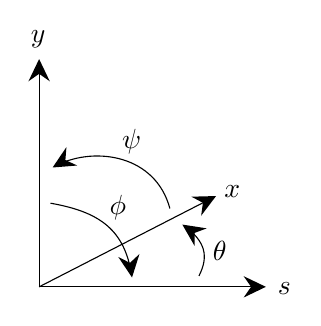
\begin{tikzpicture}[x=0.75pt,y=0.75pt,yscale=-1,xscale=1]
		%uncomment if require: \path (0,232); %set diagram left start at 0, and has height of 232
		
		%Straight Lines [id:da20170232008889133] 
		\draw    (30.75,200.25) -- (30.75,93.5) ;
		\draw [shift={(30.75,90.5)}, rotate = 90] [fill={rgb, 255:red, 0; green, 0; blue, 0 }  ][line width=0.08]  [draw opacity=0] (10.72,-5.15) -- (0,0) -- (10.72,5.15) -- (7.12,0) -- cycle    ;
		%Straight Lines [id:da7586738429193832] 
		\draw    (30.75,200.25) -- (137,200.25) ;
		\draw [shift={(140,200.25)}, rotate = 180] [fill={rgb, 255:red, 0; green, 0; blue, 0 }  ][line width=0.08]  [draw opacity=0] (10.72,-5.15) -- (0,0) -- (10.72,5.15) -- (7.12,0) -- cycle    ;
		%Straight Lines [id:da8289354712219019] 
		\draw    (30.75,200.25) -- (113.33,157.87) ;
		\draw [shift={(116,156.5)}, rotate = 152.83] [fill={rgb, 255:red, 0; green, 0; blue, 0 }  ][line width=0.08]  [draw opacity=0] (10.72,-5.15) -- (0,0) -- (10.72,5.15) -- (7.12,0) -- cycle    ;
		%Curve Lines [id:da8619095365842171] 
		\draw    (107.75,195) .. controls (111.49,187.52) and (112.39,180.04) .. (102.07,171.95) ;
		\draw [shift={(99.75,170.25)}, rotate = 34.46] [fill={rgb, 255:red, 0; green, 0; blue, 0 }  ][line width=0.08]  [draw opacity=0] (10.72,-5.15) -- (0,0) -- (10.72,5.15) -- (7.12,0) -- cycle    ;
		%Curve Lines [id:da14562765286410684] 
		\draw    (93.75,162.5) .. controls (86.83,136.71) and (58.01,132.59) .. (39.76,141.42) ;
		\draw [shift={(37.25,142.75)}, rotate = 329.74] [fill={rgb, 255:red, 0; green, 0; blue, 0 }  ][line width=0.08]  [draw opacity=0] (10.72,-5.15) -- (0,0) -- (10.72,5.15) -- (7.12,0) -- cycle    ;
		%Curve Lines [id:da5921182448586806] 
		\draw    (75.01,192.73) .. controls (71.13,171.98) and (58.98,163.96) .. (36.25,159.95) ;
		\draw [shift={(75.5,195.75)}, rotate = 261.96] [fill={rgb, 255:red, 0; green, 0; blue, 0 }  ][line width=0.08]  [draw opacity=0] (10.72,-5.15) -- (0,0) -- (10.72,5.15) -- (7.12,0) -- cycle    ;
		
		% Text Node
		\draw (113.25,177.15) node [anchor=north west][inner sep=0.75pt]    {$\theta $};
		% Text Node
		\draw (25.5,75.65) node [anchor=north west][inner sep=0.75pt]    {$y$};
		% Text Node
		\draw (118.75,150.15) node [anchor=north west][inner sep=0.75pt]    {$x$};
		% Text Node
		\draw (144.5,197.15) node [anchor=north west][inner sep=0.75pt]    {$s$};
		% Text Node
		\draw (69.5,123.19) node [anchor=north west][inner sep=0.75pt]    {$\psi $};
		% Text Node
		\draw (63.48,154.9) node [anchor=north west][inner sep=0.75pt]    {$\phi $};
	\end{tikzpicture}
	\caption{Rotation directions in the beam coordinate system (right-handed system).}\label{fig:beam-rotations}
\end{figure}

The longitudinal momentum is
\[
	p_z = \sqrt{(1 + \delta)^2 - p_x^2 - p_y^2}.
\]

\subsubsection{X Rotation}

We define a scaling factor $\kappa$ arising from the coordinate system being tilted by $\phi$ about the $x$-axis:
\[
\kappa := 1 - \frac{\tan\phi \; p_y}{p_z}.
\]
The coordinate updates can be described as follows:
\[
y \leftarrow \frac{y}{\kappa \cos\phi}, \quad p_y \leftarrow p_y \cos\phi + p_z \sin\phi,
\]

\[
x \leftarrow x + \frac{y p_x \tan\phi}{\kappa p_z}, \quad \zeta \leftarrow \zeta - \frac{y \tan\phi \left(1 + \beta_0 p_t \right)}{\kappa p_z}.
\]

\subsubsection{Y Rotation}\label{sec:Yrotation}

We define a scaling factor $\kappa$ arising from the coordinate system being tilted by $\theta$ about the $y$-axis:

\[
\kappa := 1 + \frac{\tan\theta \; p_x}{p_z}.
\]

The coordinate updates can be described as follows (which can be verified with \cite{forest99}, noting the opposite convention of the angle $\theta$):

\[
x \leftarrow \frac{x}{\kappa \cos\theta}, 
\quad 
p_x \leftarrow p_x \cos\theta - p_z \sin\theta,
\]

\[
y \leftarrow y - \frac{x\,p_y\,\tan\theta}{\kappa\,p_z}, 
\quad 
\zeta \leftarrow \zeta + \frac{x\,\tan\theta\,(1 + \beta_0 p_t)}{\kappa\,p_z}.
\]

\subsubsection{S Rotation}

We perform a rotation in the $x$-$y$ plane by an angle $\psi$:

\[
x \leftarrow x \cos\psi + y \sin\psi,
\quad
y \leftarrow -x \sin\psi + y \cos\psi,
\]

\[
p_x \leftarrow p_x \cos\psi + p_y \sin\psi,
\quad
p_y \leftarrow -p_x \sin\psi + p_y \cos\psi.
\]

\subsection{Multipole fringe field}

The fringe field effect for multipole magnets is implemented as described in 
\cite{forest99}.

\begin{align}
f_\pm &\approx 
\mp \Re \frac{c_n (x + i y)^n}{4 (n+1)(1+\delta)} 
\left\{ x p_x + y p_y + i \frac{n+2}{n} (x p_y - y p_x) \right\} 
\label{eq:fpm}
\\[1ex]
&= \frac{p_x f^x + p_y f^y}{1+\delta}.
\nonumber
\end{align}
The functions $f^x$ and $f^y$ depend on position only. 
The characteristic function is chosen so as to depend on the final momenta:
\begin{equation}
S(\vec{x}, \vec{p}^f) = \vec{x} \cdot \vec{p}^f - \frac{p_x^f f^x + p_y^f f^y}{1+\delta}.
\label{eq:characteristic}
\end{equation}
The resulting system is:
\begin{subequations}
\label{eq:system}
\begin{align}
x^f &= x - \frac{f^x}{1+\delta} \label{eq:xf} \\[0.5ex]
p_x &= p_x^f - \frac{p_x^f (\partial_x f^x) + p_y^f (\partial_x f^y)}{1+\delta} \label{eq:fringe_px} \\[0.5ex]
y^f &= y - \frac{f^y}{1+\delta} \label{eq:yf} \\[0.5ex]
p_y &= p_y^f - \frac{p_x^f (\partial_y f^x) + p_y^f (\partial_y f^y)}{1+\delta} \label{eq:fringe_py} \\[0.5ex]
\delta^f &= \delta \label{eq:deltaf} \\[0.5ex]
\ell &= \ell^f + \frac{p_x^f f^x + p_y^f f^y}{(1+\delta)^2}. \label{eq:l}
\end{align}
\end{subequations}
It is solved by inverting Eqs.~\eqref{eq:fringe_px} and \eqref{eq:fringe_py}
simultaneously for the final transverse momenta.

\subsection{Quadrupolar correction for wedge and Y rotation}

If the wedge or Y rotation take place in the presence of a quadrupole field,
the following correction is applied to the transverse momenta:
\begin{align}
p_x^f &= p_x - k_1 x^2 \theta + k_1 \frac{y^2}{2} \theta 
\label{eq:pxf}
\\
p_y^f &= p_y + k_1 x y \theta
\label{eq:pyf}
\end{align}
This correction is a perturbation of the wedge or Y rotation, and can in theory be applied using any integration scheme. It is currently implemented as a kick-drift approximation.

\subsubsection*{Derivation}
(derived by S. Van der Schueren based on the MAD-X/PTC \cite{madsite} source code)

In a curved reference frame (dropping terms of order $\mathcal{O}(y^4)$):
\begin{equation}
H_\tau = \frac{p_\tau}{\beta_0} - (1 + h x) 
\left( 
\sqrt{(1+\delta)^2 - p_x^2 - p_y^2} 
- \frac{x + \frac{h}{2} x^2}{1 + h x} b_1 + k_1 \frac{y^2}{2} - \frac{k_1 h x^3}{3} + \frac{k_1 x^2}{2(hx+1)}
\right)
\label{eq:Htau}
\end{equation}
which we can split in perturbation theory in a drift-like part $H_0$ and a kick-like part $H_1$:
\begin{align}
H_0 &= \frac{p_\tau}{\beta_0} - (1 + h x)\sqrt{(1+\delta)^2 - p_x^2 - p_y^2} + \left( x + \frac{h}{2}x^2 \right) b_0 
\label{eq:H1}
\\
H_2 &= -(1 + h x) k_1 \frac{y^2}{2} + \left( k_1 h \frac{x^3}{3} + k_1 \frac{x^2}{2} \right)
\label{eq:H2}
\end{align}

The Hamiltonian $H_0$ leads to the dipole wedge \ref{sec:DipoleWedge} (or a dynamical rotation \ref{sec:Yrotation} if $b_0 = 0$) when taking the limit $1/h \to 0, \, s \to 0, \, s h \to \theta$ . 
The Hamiltonian $H_1$ has equations of motion:
\begin{align}
p_x' &= -\frac{\partial H_2}{\partial x} 
= h k_1 \frac{y^2}{2} - h k_1 x^2 - k_1 x 
\label{eq:pxprime}
\\
p_y' &= -\frac{\partial H_2}{\partial y} 
= (1 + h x) k_1 y 
\label{eq:pyprime}
\end{align}
which gives integrated equations:
\begin{align}
p_x(s) &= p_x + h k_1 \frac{y^2}{2} s - h k_1 x^2 s - k_1 x s 
\label{eq:pxs}
\\
p_y(s) &= p_y + (1 + h x) k_1 y s 
\label{eq:pys}
\end{align}
Taking the limit to $1/h \to 0, \, s \to 0, \, s h \to \theta$ as for the dipole wedge we find the expressions for the quadrupole wedge.





\chapter{Linear optics calculations}
\label{opt}
Optics calculation are needed to study the motion around the closed orbit. By defining $z$ as the vector of $2 k$ coordinates,  
\begin{align}\label{opt:eqn:1}
z&=(z_1,\ldots,z_{2k})^T=(x-x_0,p_x-p_{x0},y-y_0,p_y-p_{y0},\tau-\tau_0,p_\tau-p_{\tau0})^T
\end{align}
one can define linear transfer maps (e.g. $M_{1\to 2}$ that propagates coordinates between two points $s_1$, $s_2$) and the one-turn map (e.g. $M_1$ that combines the effects for one turn starting from $s_1$):
\begin{align}\label{opt:eqn:2}
z(s_2)&= M_{1\to 2} z(s_1) & z(C+s_1) &= M_1 z(s_1).
\end{align}
In the following we will describe the optics calculation based on the Ripken formalism described in \cite{willeke88}. A good summary is also given in the MAD8 physics manual \cite{mad8phys}.

\section{Diagonalisation of one-turn matrix}
\label{opt:sec:1}
Since the matrices derive from symplectic maps, the eigenvalue spectrum of the one-turn map $M$ consists of 2$k$ distinct eigenvalues and linearly independent eigenvectors. In addition, for the motion to be stable the eigenvalues $\lambda_k^{\pm}$ with eigenvectors $v_k^{\pm}$ have to be complex \cite{willeke88}:
\begin{align}
M v_k^\pm  =  \lambda_k^\pm v_k^\pm, \ k=1,\ldots, 3 \\
v_k^+=(v_k^-)^*, \quad \lambda_k^+=(\lambda_k^-)^*, \quad |\lambda_k^{\pm}|=1
\end{align}
As the eigenvectors are linearly independent $M$ can be diagonalized with
\begin{align}
M &= V \Lambda V^{-1},
\end{align}
where $V$ consists of the eigenvectors and $\Lambda$ of the eigenvalues:
\begin{align}
V=&\left(
\begin{array}{cccc}
v^+_{1,1} & v^-_{1,1} & \cdots & v^-_{3,1}\\
v^+_{1,2} & v^-_{1,2} & \cdots & v^-_{3,2}\\
\vdots    & \vdots    & \vdots & \vdots \\
\end{array}
\right)  &
\Lambda=&\left(
\begin{array}{cccc}
\lambda^+_1 &    & &\\
& \lambda^-_1 & &\\
& & \ddots & \\
& & & \lambda^-_3
\end{array}
\right)
\end{align}
for which $v^{\pm}_{i,j}$ is the component $j$ of eigenvector $v_i^{\pm}$.

The same calculation can be carried out with real numbers by the following definitions:
\begin{align}\
v_k^\pm &= a_k\pm ib_k, & \lambda_k^\pm &= \cos \mu_k \pm i \sin \mu_k, &
\mu_k, a_k, b_k \in \mathbb{R}
\end{align}
such that:
\begin{align}\label{opt:eqn:1:1}
M=&W R W^{-1}
\end{align}
with
\begin{align}
R=R(\mu_k)=&\left(
\begin{array}{ccccc}
\cos \mu_1 & \sin \mu_1  &  & &\\
-\sin \mu_1 & \cos \mu_1 &  & &\\
&    & \ddots & &\\
& & & \cos \mu_3 & \sin \mu_3 \\
& & & -\sin \mu_3 & \cos \mu_3 \\
\end{array}
\right), \\
W=&\left(
\begin{array}{ccccc}
a_{1,1} & b_{1,1} & \cdots & a_{3,1} & b_{3,1} \\
a_{1,2} & b_{1,2} & \cdots & a_{3,2} & b_{3,2} \\
\vdots    & \vdots    & \vdots & \vdots\\
a_{1,6} & b_{1,6} & \cdots & a_{3,6} & b_{3,6} \\
\end{array}
\right)
\end{align}
Usually $\mu_k$ is written as $\mu_k=2\pi Q_k$, where $Q_k$ is then the tune of the mode $k$.
\section{Normalisation of eigenvectors}
\label{opt:sec:2}
By convention, the eigenvectors and values are normalized, sorted and rotated so that the following three conditions are fulfilled:
\begin{enumerate}
\item Plane 1 is associated with the horizontal, plane 2 with the vertical and plane 3 with the longitudinal plane. This is achieved by first normalizing the eigenvectors $v_k^{\pm}$ and then sorting them so that:
\begin{align}\label{opt:eqn:2:1}
|v_{j,2j-1}^{+}| =|v_{j,2j-1}^{-}| = \max_{k=1,2,3} v_{k,j}, \quad j=1,\ldots, 3
\end{align}
\item The eigenvectors are then rotated with a phase term $\psi_k$
\begin{align}
v_k& \to v_k \exp(i \psi_k) 
\end{align}
such that
\begin{align}\label{opt:eqn:2:2}
\mathrm{angle}(v_{k,2k-1}^{+})=0 \leftrightarrow \psi_k=-\mathrm{angle}(v_{k,2k-1}^{+})
\end{align}
In real space, Eqn.~\ref{opt:eqn:2:1} and \ref{opt:eqn:2:2} then become equivalent to:
\begin{align}
|a_{j,2j-1}| &=\max_{k=1,2,3} |a_{k,j}|,& b_{j,2 j-1}&=0, & j=1,\ldots, 3
\end{align}
This has the effect that a particle with $x=0$ is transformed to $\tilde x$ in the normalized phase space.
\item The sign of $b_{k,j}$ is fixed by the symplectic condition on $W$
\begin{align}
W^T S W = S
\end{align}
with $S$ defined as
\begin{align}
S&=\left(
\begin{array}{ccc}
0 & 1  &  \\
-1 & 0  &  \\
&    & \ddots \\
\end{array} 
\right)
\end{align}
which is equivalent to:
\begin{align}\label{opt:eqn:2:3}
a_k^T \cdot S \cdot b_k &=1, \quad b_k^T \cdot S \cdot a_k =-1, & \text{ for } k=l\nonumber\\
a_k^T \cdot S \cdot b_l &=0, & \text{ for }  k\not=l\\
a_k^T \cdot S \cdot a_l &=0, \quad b_k^T \cdot S \cdot b_l =0,  & k,l=1,\ldots,3 \nonumber
\end{align}
Eqn.~\ref{opt:eqn:2:3} yields that in phase space $a_k$ is thus obtained by an anticlockwise rotation of $b_k$ by $\pi/2$ and a scaling of its length with $|a_k|=\frac{1}{|b_k|}$.
\end{enumerate}
\section{Conversion to normalized coordinates}
\label{opt:sec:3}
We will show in the following that in the normalized phase space the propagation of particle coordinates $z(s)$ from $s_1$ to $s_2$ is just a rotation by an angle $\phi_k$ in the $k=1,\ldots,3$ planes, while the amplitude $I_k$ and initial phase $\phi_{k,0}$ stay constant, explicitly $z(s)$ is then given by:
\begin{align}\label{opt:eqn:3:3}
z(s)=\sum_{k=1}^3 \sqrt{2I_k}\left(
a_k(s) \cos \left(\phi_{k,0} + \phi_k(s)\right) -
b_k(s) \sin \left(\phi_{k,0} + \phi_k(s)\right)
\right) 
\end{align}
and
\begin{align}
z(s_2)&=W(s_2)R(\phi_k)W(s_1)^{-1}z(s_1), \\
&\hspace{30pt} \text{ with } \phi_k=\phi_k(s_2)-\phi_k(s_1)\nonumber
\end{align}
This implies that one turn is simply a rotation by $\phi_k=2\pi Q_k$ where $Q_k$ is the tune of the mode $k$. In the transverse plane the tune ($Q_{I,II}$) is usually positive and the particles rotate clockwise, while in the longitudinal plane the tune ($Q_{III}$) is negative above $\gamma_T$ leading to an anticlockwise rotation.

For the derivation the following steps are needed:
\begin{enumerate}
\item The effect of one turn on the normalized variable $\tilde z(s)=W^{-1}(s) z(s)$ is a rotation:
\begin{align}\label{opt:eqn:3:1}
\tilde z(C+s) = W^{-1}z(s+C)\overset{(\rm Eqn.\ref{opt:eqn:1:1})}{=}W^{-1}WRW^{-1}z(s)= R\tilde z(s),
\end{align}
As $M$ and $R$ are symplectic also $W$ is symplectic, and its inverse is thus given by $S^{-1}W^{T}S$, explicitly:
\begin{align}
W^{-1}&=
\left(
\begin{array}{cccccc}
b_{12} & - b_{11} &   b_{14} & - b_{13} &   b_{16} & - b_{15}\\
- a_{12} &   a_{11} & - a_{14} &   a_{13} & - a_{16} &   a_{15}\\
b_{22} & - b_{21} &   b_{24} & - b_{23} &   b_{26} & - b_{25}\\
- a_{22} &   a_{21} & - a_{24} &   a_{23} & - a_{26} &   a_{25}\\
b_{32} & - b_{31} &   b_{34} & - b_{33} &   b_{36} & - b_{35}\\
- a_{32} &   a_{31} & - a_{34} &   a_{33} & - a_{36} &   a_{35}\\
\end{array}
\right)
\label{eq:winv}
\end{align}
\item The one-turn map and $W$-matrix can be propagated from $s_1$ to $s_2$ by
\begin{align}
M_2&=M_{1 \to 2} M_1 M^{-1}_{1 \to 2}  &
W_2&=M_{1 \to 2} W_1
\end{align}
As Eqn.~\ref{opt:eqn:3:1} represents a similarity transformation, the eigenvalues are thus independent of the position $s$ and as the rotation matrix $R$ consists of the eigenvalues of $M$, the angle of the rotation $\mu_k=2\pi Q_k$ is thus also independent of $s$.

\item As Eqn.~\ref{opt:eqn:1:1} represents a basis transformation from the standard $\mathbb{R}^2$ basis to the eigenvector basis, the vectors $a_k$ and $b_k$ are projected onto (Eqn.~\ref{opt:eqn:2:3}):
\begin{align}\label{opt:eqn:3:2}
\tilde a_1=W^{-1}a_1&=-SW^TSa_1\nonumber\\
&=-S(a_1Sa_1,b_1Sa_1,\ldots,b_3Sa_1)^T=(1,0,\ldots,0)\nonumber\\
\tilde b_1=W^{-1}b_1&=-SW^TSb_1\nonumber\\
&=-S(a_1Sb_1,b_1Sb_1,\ldots,b_3Sb_1)^T=(0,1,\ldots,0)\\
\cdots & \nonumber\\
\tilde b_3=W^{-1}b_3&=-SW^TSb_3\nonumber\\
&=-S(a_1Sb_3,b_1Sb_3,\ldots,b_3Sb_3)^T=(0,0,\ldots,1)\nonumber
\end{align}
in the normalized phase space.
\item From Eqn.~\ref{opt:eqn:3:1} it follows that the amplitude $I_k$ and initial phase $\phi_{k0}$ of $\tilde z=W^{-1}z=(\tilde z_{a_1},\tilde z_{b_1},\ldots,\tilde z_{b_3})$ 
\begin{align}
I_k&=\frac{(\tilde z_{a_k})^2 +(\tilde z_{b_k})^2}{2}, \quad k=1,\ldots,3\label{opt:eqn:20a}\\
\tan\phi_{k0}&=-\frac{\tilde z_{b_k}}{\tilde z_{a_k}} \label{opt:eqn:20b}
\end{align}
are constants of the motion.
%, which is illustrated in Fig.~\ref{opt:fig:1}.
%\begin{figure}[h]
%	\centering
%	\includegraphics{normalized_phase_space_cropped.pdf}
%	\caption{Normalized phase space.\label{opt:fig:1}}
%\end{figure}
The initial phase is defined with a minus sign in view of the definition of the Twiss parameters, where the initial phase is then added (and not subtracted) to the phase advance. The components of $\tilde z$ are then explicitly given by:
\begin{align}
\tilde z_{a_k}&= \sum_{j=1}^3  b_{k,2j} z_{2j-1}- b_{k,2j-1} z_{2j}, \quad k=1,\ldots,3\\
\tilde z_{b_k}&= \sum_{j=1}^3 a_{k,2j-1} z_{2j}- a_{k,2j} z_{2j-1}, \quad k=1,\ldots,3.
\end{align}
An arbitrary vector $z(s)$ can thus be written in the following form:
\begin{align}
 z(s)&=W(s)\tilde z(s)\nonumber\\
 &=W(s)\left(\sum_{k=1}^{3}\tilde z_{a_k}\tilde a_k + \tilde z_{b_k}\tilde b_k\right)\nonumber\\
 &=\sum_{k=1}^{3}\tilde z_{a_k}W(s)\tilde a_k + \tilde z_{b_k}W(s)\tilde b_k\overset{\rm Eqn.~\ref{opt:eqn:3:2}}{=}\sum_{k=1}^{3}\tilde z_{a_k}a_k + \tilde z_{b_k}b_k\nonumber\\
 &\overset{\rm Eqns.~\ref
 	{opt:eqn:20a},\ref{opt:eqn:20b}}=\sum_{k=1}^{3}\sqrt{2I_k}\left(a_k\cos{\phi_{k0}}-b_k\sin{\phi_{k0}}\right)
\end{align}
\end{enumerate}

\section{Twiss parameters}
\label{opt:sec:4}
In the following the parameter $k$ will always be used for the mode $k$ and the parameter
$j=1,2,3$ for the horizontal ($x,p_x$), vertical ($y,p_y$) and longitudinal plane
$(\zeta,\delta)$ in the phase space. $z_{2j-1}$ then stands for the coordinates $(x,y,\zeta$)
and $z_{2j}$ for $(p_x,_y,\delta$).

The Twiss parameters can be introduced by writing the components of the eigenvector basis
$(a_k(s),b_k(s))$ as the product of two envelope functions $\sqrt{\beta_{k,j}(s)}$,
$\sqrt{\gamma_{k,j}(s)}$ and phase functions $\phi_{k,j}(s)$, $\bar\phi_{k,j}(s) = \phi_{k,j}(s) - \arctan(1/\alpha_{k,j})$,
also called Twiss parameters or lattice functions, with
\begin{align}
a_{k,2j-1}(s)&=\sqrt{\beta_{k,j}(s)}\cos{\phi_{k,j}(s)},\nonumber\\ b_{k,2j-1}(s)&=\sqrt{\beta_{k,j}(s)}\sin{\phi_{k,j}(s)}, \ k,j=1,\ldots,3, \label{opt:eqn:4:1}\\
a_{k,2j}(s)&=\sqrt{\gamma_{k,j}(s)}\cos{\bar\phi_{k,j}(s)}, \nonumber\\
b_{k,2j}(s)&=\sqrt{\gamma_{k,j}(s)}\sin{\bar\phi_{k,j}(s)}, \ k,j=1,\ldots,3 \label{opt:eqn:4:2}
\end{align}
where $\beta_{k,j}(s), \alpha_{k,j}(s), \gamma_{k,j}(s)$ represent the projection of the ellipse of mode $k$ on the plane of coordinates $z_{2k-1}-z_{2k}$. 
%(see Fig.~\ref{opt:fig:2})
%\begin{figure}[!ht]
%	\centering
%	\includegraphics[width=1.0\linewidth]{ripken_phase_space_ellipse.png}
%	\caption{Projection of lattice function in the $z-z'$ plane.\label{opt:fig:2}}
%\end{figure}

Using Eqns.~\ref{opt:eqn:3:3}, \ref{opt:eqn:4:1}, \ref{opt:eqn:4:2} and $\cos(x+y)=\cos x\cos y-\sin x\sin y$, the coordinates $z(s)$ can be expressed by:
\begin{align}
z_{2j-1}(s)&=\sum_{k=1}^3 \sqrt{2I_k
\beta_{k,j}(s)}\cos{(\phi_{k,j}(s)+\phi_{k,0})}\\
z_{2j}(s)&=\sum_{k=1}^3 \sqrt{2I_k
\gamma_{k,j}(s)}\cos{(\bar\phi_{k,j}(s)+\phi_{k,0})}, \ j=1,\ldots,3
\end{align}
Conversely the lattice functions can also be expressed by $a_k$ and $b_k$ with
\begin{align}
\beta_{k,j}(s)&=a_{k,2j-1}(s)^2 +b_{k,2j-1}(s)^2 \\
\alpha_{k,j}(s)&=- a_{k,2j-1}(s)a_{k,2j}(s) -b_{k,2j-1}(s)b_{k,2j}(s) \\
\gamma_{k,j}(s)&=a_{k,2j}(s)^2 +b_{k,2j}(s)^2,
\end{align}
The well known relations between the lattice functions
\begin{align}
\sum_{j=1}^3\beta_{k,j}\phi_{k,j}'&=1 \\
\gamma_{k,j}&=\frac{\beta_{k,j}^2\phi_{k,j}'^2+\alpha_{k,j}^2}{\beta_{k,j}}, \text{ with  }\\
\alpha_{k,j}&:=-\frac{1}{2}\beta_{k,j}'
\end{align}
can then be derived with the help of the normalization condition (Eqn.~\ref{opt:eqn:2:3})
\begin{align}
a_k^TSb_k=1
\end{align}
by the following steps:
\begin{enumerate}
\item As $x'=\frac{dx}{ds},\ y'=\frac{dy}{ds}$ and $\delta=\frac{d\zeta}{ds}$ the following relations hold also for $a_k$ and $b_k$:
\begin{align}
a_{k,2j}=a_{k,2j-1}'&=\frac{d}{ds}(a_{k,2j-1}), \\
b_{k,2j}=b_{k,2j-1}'&=\frac{d}{ds}(b_{k,2j-1}),\ k,j=1,\ldots,3 
\end{align}
\item The normalization condition Eqn.~\ref{opt:eqn:2:3} can then be written as
\begin{align}
a_k^TSb_k&=\sum_{j=1}^3\sqrt{\beta_{k,j}}\cos{\phi_{k,j}}\left(\sqrt{\beta_{k,j}}\sin{\phi_{k,j}}\right)'\nonumber\\
& \qquad -\left(\sqrt{\beta_{k,j}}\cos{\phi_{k,j}}\right)'\sqrt{\beta_{k,j}}\sin{\phi_{k,j}}\nonumber\\
&=\sum_{j=1}^3\beta_{k,j}\phi_{k,j}'\nonumber\\
&=1 \label{opt:eqn:4:3}
\end{align}
Note that Eqn.~\ref{opt:eqn:4:3} yields the the following relation between the phase advance $\phi$ and $\beta$ in 2D:
\begin{align}
\phi(s)=\phi(0)+\int_{s_0}^s\frac{1}{\beta(\bar s)}d\bar s
\end{align}
\item Using the abbreviation $\alpha_{k,j}:=-\frac{1}{2}\beta_{k,j}$, one finds for each mode $k$ and plane $j$
\begin{align}
\sqrt{\gamma_{k,j}}\cos{\phi_{k,j}}&=a_{k,2j}=a_{k,2j-1}'=(\sqrt{\beta_{k,j}}\cos{\phi_{k,j}})' &\quad (1)\nonumber\\
\sqrt{\gamma_{k,j}}\sin{\phi_{k,j}}&=b_{k,2j}=b_{k,2j-1}'=(\sqrt{\beta_{k,j}}\sin{\phi_{k,j}})' &\quad (2)\nonumber\\
\overset{(1)^2+(2)^2}{\Rightarrow} \gamma_{k,j}&=\frac{\beta_{k,j}^2\phi_{k,j}'^2+\alpha_{k,j}^2}{\beta_{k,j}}, \quad k,j=1,\ldots,3 &
\end{align}
which simplifies in the 2D case to:
\begin{align}
\gamma\overset{\rm Eqn.~\ref{opt:eqn:4:3}}{=}\frac{1+\alpha^2}{\beta}
\end{align}
\end{enumerate}

\section{Transformation to normalized coordinates}

The $W$ matrix can be used to transform normalized coordinate into physical coordinates and viceversa:

\begin{equation}
\left(\begin{array}{l}
x \\
p_x \\
y \\
p_y \\
\zeta \\
p_\zeta
\end{array}\right)
=
W
\left(\begin{array}{l}
\hat{x} \\
\hat{p}_x \\
\hat{y} \\
\hat{p}_y \\
\hat{\zeta} \\
\hat{p}_\zeta
\end{array}\right)
=
W
\left(\begin{array}{l}
\sqrt{\varepsilon_x} \tilde{x} \\
\sqrt{\varepsilon_x} \tilde{p}_x \\
\sqrt{\varepsilon_y} \tilde{y} \\
\sqrt{\varepsilon_y} \tilde{p}_y \\
\sqrt{\varepsilon_\zeta} \tilde{\zeta} \\
\sqrt{\varepsilon_\zeta} \tilde{p}_\zeta
\end{array}\right)
\label{eq:norm_coord}
\end{equation}
where 
\begin{equation}
\left(\begin{array}{llllll}\tilde{x} & \tilde{p}_x & \tilde{y} & \tilde{p}_y & \tilde{\zeta} & \tilde{p}_\zeta\end{array}\right)
\end{equation}
are normalized coordinates in sigmas and $\varepsilon_x$, $\varepsilon_y$ and $\varepsilon_\zeta$ are the geometric emittances.

\section{Action, amplitude and emittance}

We define the action associated to the three modes:
\begin{align}
J_x = \frac{\hat{x}^2 + \hat{p}^2_x}{2},
\quad
J_y = \frac{\hat{y}^2 + \hat{p}^2_y}{2},
\quad
J_\zeta = \frac{\hat{\zeta}^2 + \hat{p}^2_\zeta}{2}
\label{eq:action}
\end{align}

The corresponding amplitudes are defined such that:
\begin{align}
A_x &= \sqrt{\hat{x}^2 + \hat{p}^2_x} = \sqrt{2J_x}, \label{eq:ampl_x}\\
A_y &= \sqrt{\hat{y}^2 + \hat{p}^2_y} = \sqrt{2J_y}\\
A_\zeta &= \sqrt{\hat{\zeta}^2 + \hat{p}^2_\zeta} = \sqrt{2J_\zeta}
\end{align}

A Gaussian distribution is defined such that the density with respect to each action can be written as:
\begin{equation}
f(J_x) = K e^{J_x/\varepsilon_x}
\end{equation}
where the emittance $\varepsilon_x$ can be written as:
\begin{equation}
\varepsilon_x = <J_x> = \int J_x f(J_x) \,dJ_x
\end{equation}


\section{Dispersion and crab dispersion}

For a particle having no betatron amplitude ($\hat{x} = \hat{p}_x =\hat{y} =\hat{p}_y=0$) we can write:

\begin{align}
x &= W_{15}\hat{\zeta} + W_{16}\hat{p}_\zeta \label{eq:crab_x}\\
\zeta &= W_{55}\hat{\zeta} + W_{56}\hat{p}_\zeta \label{eq:crab_zeta}\\
p_\zeta &= W_{65}\hat{\zeta} + W_{66}\hat{p}_\zeta \label{eq:crab_pzeta}
\end{align}


\subsection{Dispersion}
The dispersion is:
\begin{equation}
D_{x}^{p_\zeta} = \frac{dx}{d \delta} \quad \text{for } \zeta=0
\end{equation}

By imposing $\zeta = 0$ in Eq.\,\ref{eq:crab_zeta} we obtain:

\begin{equation}
\hat{\zeta} = - \frac{W_{56}}{W_{55}}\hat{p_\zeta}
\label{eq:crab_zeta_pzeta}
\end{equation}

We replace in Eq.\,\ref{eq:crab_pzeta}:

\begin{equation}
  \hat{p}_\zeta = \left( W_{66}\ -  \frac{W_{65}W_{56}}{W_{55}} \right)^{-1}p_\zeta
\end{equation}

From Eq.\,\ref{eq:crab_zeta_pzeta} we obtain:
\begin{equation}
\hat{\zeta} = - \frac{W_{56}}{W_{55}}\left( W_{66}\ -  \frac{W_{65}W_{56}}{W_{55}} \right)^{-1} p_\zeta
\end{equation}

Replacing the last two into Eq.\,\ref{eq:crab_x} we obtain:

\begin{equation}
x = \left(W_{16} -\frac{W_{15}W_{56}}{W_{55}}\right)\left( W_{66}\ -  \frac{W_{65}W_{56}}{W_{55}} \right)^{-1} p_\zeta
\end{equation}

which gives the dispersion:
\begin{equation}
D_{x}^{p_\zeta} = \left(W_{16} -\frac{W_{15}W_{56}}{W_{55}}\right)\left( W_{66}\ -  \frac{W_{65}W_{56}}{W_{55}} \right)^{-1}
\end{equation}

A similar type of calculation can be done for the other planes, and for the transverse momentum dispersion, obtaining $D_{px}^{p_\zeta}$:
which gives the dispersion:
\begin{equation}
D_{px}^{p_\zeta} = \left(W_{26} -\frac{W_{25}W_{56}}{W_{55}}\right)\left( W_{66}\ -  \frac{W_{65}W_{56}}{W_{55}} \right)^{-1}
\end{equation}

\begin{equation}
D_{y}^{p_\zeta} = \left(W_{36} -\frac{W_{35}W_{56}}{W_{55}}\right)\left( W_{66}\ -  \frac{W_{65}W_{56}}{W_{55}} \right)^{-1}
\end{equation}

\begin{equation}
D_{py}^{p_\zeta} = \left(W_{46} -\frac{W_{45}W_{56}}{W_{55}}\right)\left( W_{66}\ -  \frac{W_{65}W_{56}}{W_{55}} \right)^{-1}
\end{equation}

\subsection{Crab dispersion}

The crab dispersion is:
\begin{equation}
D_x^\zeta = \frac{dx}{dz} \quad \text{for } p_\zeta=0
\end{equation}

By imposing $p_\zeta = 0$ in Eq.\,\ref{eq:crab_pzeta} we obtain:

\begin{equation}
\hat{p}_\zeta = - \frac{W_{65}}{W_{66}}\hat{\zeta}
\label{eq:crab_pzeta_zeta}
\end{equation}

We replace in Eq.\,\ref{eq:crab_zeta}:

\begin{equation}
\hat{\zeta} = \left( W_{55}\ -  \frac{W_{56}W_{65}}{W_{66}} \right)^{-1}\zeta
\end{equation}

From Eq.\,\ref{eq:crab_pzeta_zeta} we obtain:
\begin{equation}
\hat{p}_\zeta = - \frac{W_{65}}{W_{66}}\left( W_{55}\ -  \frac{W_{56}W_{65}}{W_{66}} \right)^{-1} \zeta
\end{equation}

Replacing the last two into Eq.\,\ref{eq:crab_x} we obtain:

\begin{equation}
x = \left(W_{15} -\frac{W_{16}W_{65}}{W_{66}}\right)\left( W_{55}\ -  \frac{W_{56}W_{65}}{W_{66}} \right)^{-1} \zeta
\end{equation}

which gives the crab dispersion:
\begin{equation}
D_x^\zeta = \left(W_{15} -\frac{W_{16}W_{65}}{W_{66}}\right)\left( W_{55}\ -  \frac{W_{56}W_{65}}{W_{66}} \right)^{-1}
\end{equation}

A similar type of calculation can be done for the other planes, and for transverse momentum crab dispersion obtaining:
\begin{equation}
D_{p_x}^\zeta = \left(W_{25} -\frac{W_{26}W_{65}}{W_{66}}\right)\left( W_{55}\ -  \frac{W_{56}W_{65}}{W_{66}} \right)^{-1}
\end{equation}
\begin{equation}
D_{y}^\zeta = \left(W_{35} -\frac{W_{36}W_{65}}{W_{66}}\right)\left( W_{55}\ -  \frac{W_{56}W_{65}}{W_{66}} \right)^{-1}
\end{equation}
\begin{equation}
D_{p_y}^\zeta = \left(W_{45} -\frac{W_{46}W_{65}}{W_{66}}\right)\left( W_{55}\ -  \frac{W_{56}W_{65}}{W_{66}} \right)^{-1}
\end{equation}

\section{Linear betatron coupling}

The following is based on \cite{luo2004phase} and \cite{Jones:2020hhl}.
~\\~\\
In the presence of betatron coupling the transverse on-momentum motion can be written as:
\begin{equation}
\left\{\begin{array}{l}
x_n=A_{1, x} \cos \left[2 \pi Q_1(n-1)+\phi_{1, x}\right]+A_{2, x} \cos \left[2 \pi Q_2(n-1)+\phi_{2, x}\right] \\
y_n=A_{1, y} \cos \left[2 \pi Q_1(n-1)+\phi_{1, y}\right]+A_{2, y} \cos \left[2 \pi Q_2(n-1)+\phi_{2, y}\right]
\end{array}\right.
\end{equation}

We can define:
\begin{equation}
\left\{\begin{array}{l}
r_1=\left|A_{1, y}\right| /\left|A_{1, x}\right| \\
r_2=\left|A_{2, x}\right| /\left|A_{2, y}\right|
\end{array}\right.
\end{equation}

\begin{equation}
\left\{\begin{aligned}
\Delta \phi_1 & =\phi_{1, y}-\phi_{1, x} \\
\Delta \phi_2 & =\phi_{2, x}-\phi_{2, y}
\end{aligned}\right.
\end{equation}

These quantities can be obtained from the normalized W matrix as:
\begin{equation}
\left\{\begin{array}{l}
r_1=\sqrt{W_{31}^2+W_{32}^2} / W_{11} \\
r_2=\sqrt{W_{13}^2+W_{14}^2} / W_{33}
\end{array}\right.
\end{equation}

\begin{equation}
\left\{\begin{array}{l}
\Delta \phi_{1,0}=\arctan \left(W_{32} / W_{31}\right) \\
\Delta \phi_{2,0}=\arctan \left(W_{14} / W_{13}\right)
\end{array}\right.
\end{equation}

From these we can compute the following quantities as\,\cite{Jones:2020hhl}:
\begin{equation}
\left|C^{-}\right|=\frac{2 \sqrt{r_1 r_2}\left|Q_1-Q_2\right|}{\left(1+r_1 r_2\right)}
\label{eq:cmin}
\end{equation}
\begin{equation}
\chi(s) = \Delta \phi_{1,0}(s)
\end{equation}
\begin{equation}
C^-(s) = \left|C^{-}\right|e^{i\chi(s)}
\end{equation}
where $Q_1$ and $Q_2$ are the tunes of the betatron eigenmodes. Note that only the phase of $C^-(s)$ is $s$ dependent.

It is possible to prove that $C^-$ is related to the skew quadrupole strengths along the ring by the following relation:
\begin{equation}
C^{-}=\left|C^{-}\right| e^{i \chi}=\frac{1}{2 \pi} \int_0^L \sqrt{\beta_x \beta_y} k_s e^{i\left[\Phi_x-\Phi_y-2 \pi \Delta \cdot s / L\right]} d l .
\end{equation}
where $\Delta$ is the difference of the unperturbed fractional tunes.

To have a more robust estimate, Eq.\,\ref{eq:cmin} is evaluated at all $s$ positions
and averaged over the ring, as suggested in \cite{tobias_coupling_note}.

\subsection{Edwards-Teng formalism}

This section is based on \cite{mad8phys}. The full derivation can be found in
\cite{laurent_coupling_1} and \cite{laurent_coupling_2}.

Consider the linear transfer map $R$ in two degrees of freedom, partitioned into four $2\times2$ blocks:
\begin{equation}
R=
\begin{pmatrix}
A & B\\
C & D
\end{pmatrix}.
\end{equation}

The 4\,-dimensional phase space vector shall also be partitioned according
to the horizontal and vertical planes. Edwards and Teng introduce a
``symplectic rotation'':
\begin{equation}
T_\text{ET}=
\begin{pmatrix}
I\cos\phi & \overline{R}_\text{ET}\,\sin\phi\\
-\,R_\text{ET}\sin\phi & I\cos\phi
\end{pmatrix}.
\end{equation}

Here $R_\text{ET}$ is a $2 \times 2$ matrix with unit determinant,
and $\overline{R}_\text{ET}$ denotes its symplectic conjugate:
\begin{equation}
R_\text{ET}=
\begin{pmatrix}
a & b\\
c & d
\end{pmatrix},
\qquad
|R_\text{ET}|=
\left|
\begin{matrix}
a & b\\
c & d
\end{matrix}
\right|
=1,
\qquad
\overline{R}_\text{ET}=
\begin{pmatrix}
d & -b\\
-c & a
\end{pmatrix}.
\end{equation}

This leaves three free parameters for the elements of $R_\text{ET}$, and a fourth parameter $\phi$.
Edwards and Teng then determine $R_\text{ET}$ such that $R$ conjugated with $T_\text{ET}$ becomes block diagonal:
\begin{equation}
T_\text{ET}MT_\text{ET}^{-1}=
\begin{pmatrix}
E & 0\\
0 & F
\end{pmatrix}.
\end{equation}

If $\,|B+\overline{C}|<0\,$ both $\phi$ and all elements of $R_\text{ET}$ become imaginary. This may be avoided by redefining
\begin{equation}
T_\text{ET}=\frac{1}{\sqrt{\,1+|R_\text{ET}|\,}}
\begin{pmatrix}
I & \overline{R}_\text{ET}\\
-\,R_\text{ET} & I
\end{pmatrix},
\end{equation}
where all four elements of $R_\text{ET}$ are free parameters.

The solution is
\begin{equation}
R_\text{ET}=\Bigg(
\frac{1}{2}\big(\operatorname{Tr}A-\operatorname{Tr}D\big)
+\operatorname{sign}\!\big(|C+\overline{B}|\big)\,
\sqrt{|C+\overline{B}|+\frac{1}{4}\big(\operatorname{Tr}A-\operatorname{Tr}D\big)^2}
\Bigg)^{-1}\,(C+\overline{B}),
\end{equation}
and
\begin{align}
E=A-BR_\text{ET}\\
F=D+R_\text{ET}B
\end{align}

Twiss parameters of $E$ (and $F$) can be found by:
\begin{equation}
E=
\begin{pmatrix}
E_{1,1} & E_{1,2}\\
E_{2,1} & E_{2,2}
\end{pmatrix}
=
\begin{pmatrix}
\cos\mu_A + \alpha_A \sin\mu_A & \beta_A \sin\mu_A\\
-\gamma_A \sin\mu_A & \cos\mu_A - \alpha_A \sin\mu_A
\end{pmatrix}
\end{equation}

\begin{align}
&\cos\mu_A=\tfrac12\,\operatorname{tr}E, \\
&\sin\mu_A=\operatorname{sign}(E_{1,2})
\sqrt{-\,E_{1,2}E_{2,1}-\left(\frac{E_{1,1}-E_{2,2}}{2}\right)^{\!2}}\\
&\beta_A=\frac{E_{1,2}}{\sin\mu_A}\\
&\gamma_A=-\,\frac{E_{2,1}}{\sin\mu_A}\\
&\alpha_A=\frac{E_{1,1}-E_{2,2}}{2\sin\mu_A}.
\end{align}




\chapter{Counter-rotating beams}

In machines having counter-rotating beams, such as the LHC, it is useful to be able
to express beam coordinates for one of the beams in the reference frame of the other.
Furthermore it is also useful to be able to define the two sequences using the same
orientation. For the LHC, for example, the sequence of the LHC beam 2 is defined
following the orientation of the LHC beam 1. In this case the properties of the
elements are specified in such a way that the built sequence is able to backtrack
the physical beam and the sequence required to track the physical beam (usually called
Beam 4 sequence) can be obtained with suitable transformations.

\section{Reversed reference frame}
The reference frames for beam 4 and beam 2 are related by the following transformations:
\begin{align}
&\tilde{x} = -x \label{eq:rev_x}\\
&\tilde{y} = y \label{eq:rev_y}\\
&\tilde{s} = -s \label{eq:rev_s}\\
&\tilde{t} = -t \label{eq:rev_t}\\
&\tilde{\zeta} = -\zeta \label{eq:rev_zeta}\\
&\tilde{p_x} = p_x \label{eq:rev_px}\\
&\tilde{p_y} = -p_y \label{eq:rev_py}\\
&\tilde{p_\zeta} = p_\zeta \label{eq:rev_pzeta}\\
&\tilde{\delta} = \delta \label{eq:rev_delta}
\end{align}
where the tilde indicates the coordinates in the reversed reference frame.

\section{Transformation of beam elements}

The elements are tranformed in such a way that the map implements the backtrack of
the physical beam as seen in the reversed reference frame.

\subsection{Horizontal deflecting cavity}

In the case of a horizontal deflecting cavity we can proceed as follows.

For Beam 4 we can write:
\begin{equation}
\Delta p_x = V_x \sin(\phi - \omega t)
\end{equation}
and for Beam 2 we can write:
\begin{equation}
\Delta\tilde{p}_x = \tilde{V}_x \sin(\tilde{\phi} - \omega \tilde{t}),\\[4pt]
\end{equation}
Since we define the element as backtracking we can write:
\begin{equation}
\Delta \tilde{p}_x = -\,\Delta p_x
\end{equation}
where the minus sign comes from the backtracking and no additional sign change
comes from the reference frame transformation (see Eq.\,\ref{eq:rev_px}).

Combining the equations above we obtain:
\begin{equation}
\tilde{V}_x \sin(\tilde{\phi} - \omega \tilde{t}) = -\,V_x \sin(\phi - \omega t)
\end{equation}
Using Eq.\,\ref{eq:rev_t} we can write:
\begin{equation}
\tilde{V}_x \sin(\tilde{\phi} + \omega t) = -\,V_x \sin(\phi - \omega t)
\end{equation}
We choose to reverse the voltage definition since also the electric field is
expressed in the reversed reference frame:
\begin{equation}
\boxed{
\tilde{V}_x = -\,V_x
}
\end{equation}
obtaining:
\begin{equation}
\sin(\tilde{\phi} + \omega t) = \sin(\phi - \omega t)
\end{equation}
Using trigonometric properties we can write:
\begin{equation}
-\sin(-\tilde{\phi} - \omega t) = \sin(\phi - \omega t)
\end{equation}
and then:
\begin{equation}
\sin(\pi - \tilde{\phi} - \omega t) = \sin(\phi - \omega t)
\end{equation}
From this we obtain:
\begin{equation}
\boxed{
\tilde{\phi} = \pi - \phi
}
\end{equation}

\section{Vertical deflecting cavity}

The case of a vertical deflecting cavity is similar but not identical.

For Beam 4 we can write:
\begin{equation}
\Delta p_y = V_y \sin(\phi - \omega t)
\end{equation}
and for Beam 2 we can write:
\begin{equation}
\Delta\tilde{p}_y = \tilde{V}_y \sin(\tilde{\phi} - \omega \tilde{t}),\\[4pt]
\end{equation}
Since we define the element as backtracking we can write:
\begin{equation}
\Delta \tilde{p}_y = -(-\Delta p_y)
\end{equation}
where one minus sign comes from the backtracking and an additional sign change
comes from the reference frame transformation (see Eq.\,\ref{eq:rev_py}).

Combining the equations above we obtain:
\begin{equation}
\tilde{V}_y \sin(\tilde{\phi} - \omega \tilde{t}) = V_y \sin(\phi - \omega t)
\end{equation}
Using Eq.\,\ref{eq:rev_t} we can write:
\begin{equation}
\tilde{V}_y \sin(\tilde{\phi} + \omega t) = -V_y \sin(\phi - \omega t)
\end{equation}
We do not reverse the voltage definition as the vertical component of the electric
field does not change sign due to the reference frame transformation:
\begin{equation}
\boxed{
\tilde{V}_y = \,V_y
}
\end{equation}
Hence we obtain:
\begin{equation}
\sin(\tilde{\phi} + \omega t) = \sin(\phi - \omega t)
\end{equation}
Using trigonometric properties we can write:
\begin{equation}
-\sin(-\tilde{\phi} - \omega t) = \sin(\phi - \omega t)
\end{equation}
and then:
\begin{equation}
\sin(\pi - \tilde{\phi} - \omega t) = \sin(\phi - \omega t)
\end{equation}
From this we obtain:
\begin{equation}
\boxed{
\tilde{\phi} = \pi - \phi
}
\end{equation}







\chapter{Synchrotron radiation}

We collect here some relevant properties of synchrotron radiation~\cite{hofmann_2004}:

We assume $B = |B_\perp|$.

Classical particle radius:
\begin{equation}
r_0=Q^2 /\left(4 \pi \epsilon_0 m_0 c^2\right)
\end{equation}

Curvature, rigidity, field:
\begin{equation}
\frac{1}{\rho}=\frac{Q B}{p}=\frac{Q B}{m_0 c \beta \gamma}
\end{equation}

Emitted power:
\begin{equation}
P_{\mathrm{s}}=\frac{2 r_0 c^3 Q^2 \beta^2 \gamma^2 B^2}{3 m_0 c^2}
\end{equation}



Critical frequency:
\begin{equation}
\omega_{\mathrm{c}}=\frac{3 Q \beta^2 \gamma^2 B }{2 m_0}
\end{equation}

Critical energy:
\begin{equation}
E_{\gamma \mathrm{c}}=\hbar \omega_{\mathrm{c}}
=\frac{3 Q \hbar\beta^2 \gamma^2 B }{2 m_0}
\end{equation}

Number of photons per unit time:
\begin{equation}
\dot{n}_{\mathrm{s}}=\frac{15 \sqrt{3}}{8}\frac{P_{\mathrm{s}}}{E_{\gamma \mathrm{c}}} 
=\frac{60 \sqrt{3}}{72}
\frac{ r_0 c Q B}{\hbar}
\end{equation}

Average photon energy:
\begin{equation}
\left\langle E_\gamma\right\rangle=\frac{8 \sqrt{3}}{45} E_{\gamma \mathrm{c}}
=\frac{8 \sqrt{3}}{15} 
\frac{ Q \hbar\beta^2 \gamma^2 B }{2 m_0}
\end{equation}

Photon energy variance:
\begin{equation}
\left\langle E_\gamma^2\right\rangle=\frac{11}{27} E_{\gamma \mathrm{c}}^2
= 
\frac{11}{12}\frac{ Q^2\hbar^2\beta^4\gamma^4 B^2 }{ m_0^2}
\end{equation}

\begin{equation}
\left\langle \dot{n}_{\mathrm{s}} \Delta \delta ^2\right\rangle
=
\frac{\left\langle \dot{n}_{\mathrm{s}} {E_\gamma^2}
 \right\rangle} {E_0^2}
= 
\frac{11}{12}
\frac{1}{m_0^2 c^4 \gamma_0^2 }
\frac{ Q^2\hbar^2\beta^4\gamma^4 B^2 }{ m_0^2}
\frac{60 \sqrt{3}}{72}
\frac{ c Q B}{\hbar}
\frac{Q^2}{4 \pi \epsilon_0 m_0 c^2}
\end{equation}

The algorithm to generate photon energies with the appropriate distribution in described in~\cite{helmut_synrad_90}.



\section{Damping from synchrotron radiation}
\label{section:sr_damping_times}

The damping constants from synchrotron radiation can be easily obtained from magnitude of the eigenvalues of the one-turn matrix:
\begin{align}
\alpha_x &= -\log( \lvert \lambda_x \rvert)\\
\alpha_y &= -\log( \lvert \lambda_y \rvert)\\
\alpha_\zeta &= -\log( \lvert \lambda_\zeta \rvert)
\end{align}

The damping acts such that:
\begin{equation}
\frac{1}{A_x} \frac{dA_x}{dt} = - \frac{\alpha_x}{T_0} 
\end{equation}
where $T_0$ is the revolution period.
From Eq.\,\ref{eq:ampl_x} we obtain:
\begin{equation}
\frac{dJ_x}{dt} = - \frac{2\alpha_x}{T_0}  J_x
\end{equation}
By averaging over the beam distribution we obtain:
\begin{equation}
\frac{d\varepsilon_x}{dt} = - \frac{2\alpha_x}{T_0}  \varepsilon_x
\label{eq:grate_rad_damp}
\end{equation}

\section{Equilibrium emittance}

This section is based on the approach described in \cite{chao_eq_emit}.

To account for the kicks experienced by the particles due to quantum excitation we note that the transverse momentum change due to an energy kick in the direction of the particle motion can be written as:
\begin{align}
P_{x,y}^\text{new} = P_{x,y}^\text{old}  \frac{P^\text{new}}{P^\text{old}}
\end{align}

From this:
\begin{align}
P_{x,y}^\text{new} - P_{x,y}^\text{old} = P_{x,y}^\text{old}  \left(\frac{P^\text{new} - P^\text{old}}{P^\text{old}} \right) 
\end{align}

Dividing by $P_0$:
\begin{align}
\frac{P_{x,y}^\text{new} - P_{x,y}^\text{old}}{P_0} = 
\frac{P_{x,y}^\text{old}}{P_0}
\left(\frac{P^\text{new} - P^\text{old}}{P_0} \right) 
\frac{P_0}{P^\text{old}}
\end{align}

Using the accelerator coordinates definitions (Eqs.\,\ref{eq:coord1} and \ref{eq:coord2}), we obtain:
\begin{align}
\Delta p_{x,y} = \frac{p_{x,y}}{1 + \delta} \Delta \delta
\end{align}

The corresponding change in normalized coordinates can be computed from Eq.\,\ref{eq:norm_coord}:

\begin{equation}
\left(\begin{array}{l}
\Delta \tilde{x} \\
\Delta \tilde{p}_x\\
\Delta \tilde{y} \\
\Delta \tilde{p}_y \\
\Delta \tilde{\zeta} \\
\Delta \tilde{p}_\zeta
\end{array}\right)
=
W^{-1}
\left(\begin{array}{c}
0 \\
\cfrac{p_{x}}{1 + \delta} \Delta \delta \\
0 \\
\cfrac{p_{y}}{1 + \delta} \Delta \delta \\
0 \\
\Delta \delta
\end{array}\right)
\label{eq:norm_coord}
\end{equation}

Using the Eq.\,\ref{eq:winv} we obtain:
\begin{align}
&\Delta \hat{x} = \mathcal{K}_x \Delta \delta \label{eq:sr_dxhat}\\
&\Delta \hat{p}_x = \mathcal{K}_{p_x} \Delta \delta \label{eq:sr_dxphat}\\
&\Delta \hat{y} = \mathcal{K}_{y} \Delta \delta \\
&\Delta \hat{p}_y = \mathcal{K}_{p_y} \Delta \delta\\
&\Delta \hat{\zeta} = \mathcal{K}_{\zeta} \Delta \delta \\
&\Delta \hat{p}_\zeta = \mathcal{K}_{p_{\zeta}}\Delta \delta
\end{align}
where:
\begin{align}
\mathcal{K}_x &= 
\left( \cfrac{a_{11}p_{x} + a_{13}p_{y} }{1 + \delta} + a_{15}\right)\\
\mathcal{K}_{p_x} &= 
\left( \cfrac{b_{11}p_{x} + b_{13}p_{y} }{1 + \delta} + b_{15}\right)\\
\mathcal{K}_y &= 
\left( \cfrac{a_{21}p_{x} + a_{23}p_{y} }{1 + \delta} + a_{25}\right)\\
\mathcal{K}_{{p}_y} &= 
\left( \cfrac{b_{21}p_{x} + b_{23}p_{y} }{1 + \delta} + b_{25}\right)\\
\mathcal{K}_{\zeta} &= 
\left( \cfrac{a_{31}p_{x} + a_{33}p_{y} }{1 + \delta} + a_{35}\right)\\
\mathcal{K}_{p_\zeta} &= 
\left( \cfrac{b_{31}p_{x} + b_{33}p_{y} }{1 + \delta} + b_{35}\right)
\end{align}

The change in action (see Eq.\,\ref{eq:action}) associated to the first mode, due to the emission of a photon can be written as:
\begin{align}
\Delta J_x &= \frac{1}{2}\left[
\left(\hat{x} +\Delta \hat{x}\right)^2 
\left(\hat{p}_x +\Delta \hat{p}_x \right)^2 
-\hat{x}^2 - \hat{p}_x^2
\right]\\
&= \frac{1}{2}\left[
\Delta \hat{x}^2 + \Delta \hat{p}_{x}^2
+ 2 \hat{x} \Delta \hat{x} + 2 \hat{p}_{x} \Delta \hat{p}_{x} 
\right]
\end{align}

Averaging over all particles in the beam we obtain:
\begin{align}
\Delta \varepsilon_x = <\Delta J_x> = 
\frac{1}{2}\left( <\Delta \hat{x}^2> + <\Delta \hat{p}_{x}^2> \right)
\end{align}

Using Eqs.\,\ref{eq:sr_dxhat} and \ref{eq:sr_dxphat} we obtain:
\begin{align}
\Delta \varepsilon_x = <\Delta J_x> = 
\frac{1}{2}\left(\mathcal{K}^2_x + \mathcal{K}^2_{p_x}\right)<\Delta \delta^2>
\end{align}

Assuming that the kicks are uncorrelated we can obtain the emittance growth rate from quantum excitation integrating over a full turn:
\begin{align}
\left(\frac {d\varepsilon_x}{dt} \right)_\text{quant}= 
\frac{1}{2T_0c}\int_0^C\left(\mathcal{K}^2_x + \mathcal{K}^2_{p_x}\right)<\dot{N} \Delta \delta^2> \,ds
\label{eq:grate_quantum}
\end{align}
where $\dot{N}$ is the photon emission rate (number of photons per unit time), $T_0$ is the revolution period, C is the circumference.

By summing Eqs.\,\ref{eq:grate_rad_damp} and \ref{eq:grate_quantum} we obtain the total instantaneous growth rate:
\begin{align}
\frac {d\varepsilon_x}{dt} = 
\left(\frac {d\varepsilon_x}{dt}\right)_\text{damp}
+
\left(\frac {d\varepsilon_x}{dt}\right)_\text{quant}
=
- \frac{2\alpha_x}{T_0}  \varepsilon_x
+
\frac{1}{2T_0c}\int_0^C\left(\mathcal{K}^2_x + \mathcal{K}^2_{p_x}\right)<\dot{N} \Delta \delta^2> \,ds
\end{align}

By imposing the derivative to be zero we obtain the value of the equilibrium emittance:
\begin{align}
\varepsilon_x= 
\frac{1}{4\alpha_xc}\int_0^C\left(\mathcal{K}^2_x + \mathcal{K}^2_{p_x}\right)<\dot{N} \Delta \delta^2> \,ds
\label{eq:equilemi1}
\end{align}

In the ultra-relativistic approximation:
\begin{align}
<\dot{N} \Delta \delta^2> = 
\frac{<\dot{N} (\Delta E)^2>}{E_0^2}
\label{eq:equilemi2}
\end{align}

\section{Radiation integrals}

Xsuite can compute the following radiation integrals:
\begin{align}
    &I_1 = \oint \left( h_{0x} D_x + h_{0y} D_y \right)\ \dee s\\
    &I_2 = \oint |h|^2 \ \dee s\\
    &I_3 = \oint |h|^3 \ \dee s\\
    &I_{4x} = \oint \left( |h|^2 h_{0x} + 2 h_x k_1 \right) D_x\ \dee s\\
    &I_{4y} = \oint \left( |h|^2 h_{0y} - 2 h_y k_1 \right) D_y\ \dee s\\
    &I_4 = I_{4x} + I_{4y} = \oint \left[ 2k_1 \left( h_x D_x - h_y D_y \right) + |h|^2 (h_{0x}D_x + h_{0y} D_y) \right] \ \dee s\\
    &I_{5x} = \oint h^3 \curlyH_x\ \dee s\\
    &I_{5y} = \oint h^3 \curlyH_y\ \dee s
\end{align}

The following quantities are used in the calculation.
\begin{itemize}
\item Horizontal and curvature of the particle trajectory:
\begin{align}
    &h_x = \frac{B_y Q}{m_0 c \gamma}    \label{eq:curvx}\\
    &h_y = -\frac{B_x Q}{m_0 c \gamma}   \label{eq:curvy}
\end{align}
\item Total transverse curvature and relation to the transverse magnetic field:
\begin{equation}
    h = \sqrt{h_x^2 + h_y^2}
\end{equation}
which is related to the transverse magnetic field by:
\begin{equation}
    B = \sqrt{B_x^2 + B_y^2}  = h  \frac{m_0 \beta c \gamma}{Q}
    \label{eq:btocurv}
\end{equation}
\item ``Curly H'' functions:
\begin{align}
    \curlyH_x = \gamma_x D_x^2 + 2 \alpha_x D_x D_x' + \beta_x D_x'^2\\
    \curlyH_y = \gamma_y D_y^2 + 2 \alpha_y D_y D_y' + \beta_y D_y'^2
\end{align}
\item The derivative of the dispersion $D'_{x,y}$ can be obtained from the transverse
momentum dispersion $D_{p_{x,y}}$ using the relation:
\begin{equation}
    D'_{x,y} = \totder{D_{x,y}}{s} = \totder{x'}{\delta} =
      \totder{~}{\delta} \frac{p_{x,y}}{1+\delta} = (1 - \delta)D_{p_{x,y}} - p_{x,y}
    \label{eq:ddispder}
\end{equation}
\item $h_{0x}$ and $h_{0y}$ are the curvatures of the reference trajectory. The path
length on the particle trajectory is related to the path length on the reference trajectory by:
\begin{equation}
    \dee s' = (1 + h_{0x}x + h_{0y}y)\ \dee s
    \label{eq:pathlength}
\end{equation}
\end{itemize}

The radiation integrals can be used to compute the following quantities
  (where
   %$m_0$ is the particle rest mass, $Q$ is the charge of the particle, , $E_0$ is the reference energy, $\gamma$ is the relativistic gamma factor, $\delta$ is the relative deviation from the reference energy, 
   $C_0$ is the ring circumference, $r_0$ is the classical particle radius, $\hbar$ is the reduced Planck's constant)
  %  $s'$ is the arclength along the particle orbit, $s$ is the arclength along the reference orbit, $x$ ($y$) is the horizontal (vertical) coordinate, $D_x$ ($D_y$) is the dispersion in the horizontal (vertical) plane, $D_x'$ ($D_y'$) is its derivative, $h_{0x}$ ($h_{0y}$) is the curvature of the reference orbit in the horizontal (vertical) plane, $h_x$ ($h_y$) is the curvature of the particle orbit in the horizontal (vertical) plane, $k_1$ is the normalised normal quadrupole strength, $\alpha_x$, $\beta_x$ and $\gamma_x$ ($\alpha_y$, $\beta_y$ and $\gamma_y$) are the betatron functions in the horizontal (vertical) plane, $c$ is the speed of light and )
:
\begin{itemize}
    \item Momentum compaction factor (unitless):
    \begin{equation}
        \alpha_c = \frac{I_1}{C_0}
    \end{equation}

    \item Energy loss per turn [Js$^{-1}$]:
    \begin{equation}
        U_s = \frac{2}{3} c r_0 E_0 \gamma^3 I_2
    \end{equation}

    \item Damping partition numbers:
    \begin{align}
        J_x &= 1 - \frac{I_{4x}}{I_2}\\
        J_y &= 1 - \frac{I_{4y}}{I_2}\\
        J_z &= 2 + \frac{I_4}{I_2}
    \end{align}
    which satisfy Robinson's theorem:
    \begin{equation}
        J_x + J_y + J_z = 4
    \end{equation}

    \item Longitudinal damping rate in [s$^{-1}$]:
    \begin{equation}
        \alpha_\epsilon = \frac{c r_0 \gamma^3}{3 C_0} (2I_2 + I_4)
    \end{equation}

    \item Transverse damping rates in [s$^{-1}$]:
    \begin{align}
        \alpha_x &= \frac{c r_0 \gamma^3}{3C_0} (I_2 - I_{4x})\\
        \alpha_y &= \frac{c r_0 \gamma^3}{3C_0} (I_2 - I_{4y})
    \end{align}

    \item Energy spread (unitless):
    \begin{equation}
        \sigma_\delta^2 = \frac{55 \sqrt{3}}{96} \frac{\hbar \gamma^2}{m_0 c} \frac{I_3}{2I_2 + I_4}
    \end{equation}

    \item Transverse equilibrium emittances in [m rad]:
    \begin{align}
        {\epsilon_x} &= \frac{55 \sqrt{3}}{96} \frac{\hbar \gamma^2}{m_0 c} \frac{I_{5x}}{I_2 - I_{4x}}\\
        {\epsilon_y} &= \frac{55 \sqrt{3}}{96} \frac{\hbar \gamma^2}{m_0 c} \frac{I_{5y}}{I_2 - I_{4y}}
    \end{align}


\end{itemize}

\subsection{Derivations}
\subsubsection{Energy Loss and Second Radiation Integral}
\label{sec:enelossandi2}

From the instantaneous radiated power,

\begin{equation}
    P_s = \frac{2}{3}\frac{c^3 r_0 Q^2 E^2 B^2}{(m_0 c^2)^3} = \frac{2}{3} c r_0 E \gamma^3 |h|^2
    \label{eq:instpower}
\end{equation}

The energy loss per turn is obtained by integration around one turn.
\begin{equation}
U_s = \int P_s(t) \ \dee t \approx \frac{1}{c} \oint P_s(s') \ \dee s'
= \frac{2}{3} c r_0 E \gamma^3 \oint |h|^2 \ \dee s'
\end{equation}
We can assume $(h_{0x}x + h_{0y}y) \ll 1$, obtaining:
\begin{equation}
\label{eq:enelossturn}
U_s =\frac{2}{3} c r_0 E \gamma^3 I_{2}
\end{equation}
where we have defined the second radiation integral:
\begin{equation}
I_2     = \oint |h|^2 \ \dee s
\end{equation}

\subsubsection{Longitudinal Damping Rate and Fourth Radiation Integral}
\label{sec:longdampandi4}

Following Hofmann's analysis, the longitudinal damping rate can be written as \cite{hofmann_2004}:
\begin{equation}
    \alpha_\epsilon = \frac{1}{2} \frac{1}{T_\text{rev}} \totder{U_s}{E}
    \label{eq:alphadamp}
\end{equation}

We calculate:
\begin{equation}
    \totder{U_s}{E} = \frac{1}{c} \totder{}{E} \oint P_s(s') \ \dee s' = \frac{1}{c} \totder{}{E} \oint P_s \ (1 + h_{0x}x(E) + h_{0y}y(E))\ \dee s
    \label{eq:dUdEoint}
\end{equation}

Using the dispersion to express $x(E)$ and $y(E)$:
\begin{equation}
    \totder{U_s}{E} = \totder{}{E} \frac{1}{c} \oint P_s \ (1 + h_{0x}D_x \delta + h_{0y} D_y \delta)\ \dee s
\end{equation}

The derivative w.r.t. $E$ is related to the derivative w.r.t. $\delta$ by:
\begin{equation}
    \totder{}{E} = \totder{\delta}{E} \totder{}{\delta} = \totder{}{E} \left( \frac{E - E_0}{E_0} \right) \totder{}{\delta} = \frac{1}{E_0} \totder{}{\delta}
    \label{eq:ddEtodddelta}
\end{equation}

Writing out the derivative then gives:
\begin{align}
    \totder{U_s}{E} &= \frac{1}{c} \oint \totder{P_s}{E} (1 + h_{0x}D_x \delta + h_{0y} D_y \delta) + \frac{P_s}{E_0} \totder{}{\delta}(1 + h_{0x}D_x \delta + h_{0y} D_y \delta)\ \dee s \notag \\
                    &= \frac{1}{c} \oint \totder{P_s}{E} (1 + h_{0x}D_x \delta + h_{0y} D_y \delta) + \frac{P_s}{E_0} (h_{0x}D_x + h_{0y} D_y)\ \dee s
\end{align}

The derivative of $P_s$ w.r.t. $E$ can be rewritten as:
\begin{equation}
    \totder{P_s}{E} = 2 P_s \left[ \frac{1}{E} + \frac{1}{B} \left( \partder{B}{x} \totder{x}{E} + \partder{B}{y} \totder{y}{E} \right) \right]
\end{equation}

The derivatives of the positions w.r.t. $E$ are related to the dispersions through Eq.\,\ref{eq:ddEtodddelta}
\begin{align}
    \totder{x}{E} &= \frac{1}{E_0} \totder{x}{\delta} = \frac{1}{E_0} D_x\\
    \totder{y}{E} &= \frac{1}{E_0} \totder{y}{\delta} = \frac{1}{E_0} D_y
\end{align}

Using the fact that $B = \sqrt{B_x^2 + B_y^2}$, the derivatives of $B$ w.r.t. $x$ and $y$ are:
\begin{align}
    \partder{B}{x} &= \frac{B_x}{B} \partder{B_x}{x} + \frac{B_y}{B} \partder{B_y}{x}\\
    \partder{B}{y} &= \frac{B_x}{B} \partder{B_x}{y} + \frac{B_y}{B} \partder{B_y}{y}
\end{align}
The magnetic field gradients are defined as:
\begin{align}
    &\partder{B_y}{x} = \partder{B_x}{y}  = G       = \frac{\gamma_0 m_0 c}{Q_0} k_1\\
    &\partder{B_x}{x} = -\partder{B_y}{y} = \bar{G} = \frac{\gamma_0 m_0 c}{Q_0} \bar{k}_1
\end{align}

Here, $k_1$ is the normalised normal quadrupole strength and $\bar{k}_1$ is the normalised skew quadrupole strength, both in units of $1/m^2$. In the following we neglect the skew quadrupole component and we assume that for the closed orbit we can assume $\gamma\simeq\gamma_0$, obtaining:
\begin{equation}
    \totder{P_s}{E} = 2 P_s \left[ \frac{1}{E} + \frac{1}{E_0} \frac{\gamma m_0 c}{Q_0} \frac{k_1}{B^2} \left( B_y D_x + B_x D_y \right) \right]
\end{equation}

The curvatures in Eqs.\,\eqref{eq:curvx}, \eqref{eq:curvy} and \eqref{eq:btocurv} can be substituded, which gives:
\begin{equation}
    \totder{P_s}{E}
    %= 2 P_s \left[ \frac{1}{E} + \frac{1}{E_0}\frac{\gamma m_0 c}{Q} \frac{Q^2}{(\gamma m_0 c)^2} \frac{k_1}{h^2} \frac{\gamma m_0 c}{Q} \left( h_x D_x - h_y D_y \right) \right]
    = 2 \frac{P_s}{E} \left[ \frac{1}{E} + \frac{1}{E_0} \frac{k_1}{h^2} \left( h_x D_x - h_y D_y \right) \right]
    \label{eq:dPdE}
\end{equation}

Substituting Eq.\,\eqref{eq:instpower} gives:
\begin{equation}
    \totder{P_s}{E}
    % = \frac{4}{3} c r_0 E \gamma^3 |h|^2 \left[ \frac{1}{E} + \frac{1}{E_0} \frac{k_1}{h^2} \left( h_x D_x - h_y D_y \right) \right]
    = \frac{4}{3} c r_0 E \gamma^3  \left[ \frac{|h|^2}{E} + \frac{1}{E_0} k_1 \left( h_x D_x - h_y D_y \right) \right]
\end{equation}

Substituting this expression back in Eq.\,\eqref{eq:dUdEoint} gives:
\begin{align}
    \totder{U_s}{E} = \frac{2}{3} \frac{c r_0 E \gamma^3}{c} \oint \bigg[ &2\frac{|h|^2}{E}(1 + h_{0x}x + h_{0y}y) +
    2\frac{k_1}{E_0} \left( h_x D_x - h_y D_y \right)(1 + h_{0x}x + h_{0y}y) \notag\\ &+ \frac{|h|^2}{E_0} (h_{0x}D_x + h_{0y} D_y)\bigg] \ \dee s
\end{align}

The first term can be identified as $I_2$, again we assume that $h_{0x}x + h_{0y}y \ll 1$ and, as stated above on the closed orbit we assume $E/E_0 \approx 1$. Hence, we can write:
\begin{align}
    \totder{U_s}{E} = &\frac{2}{3} r_0 \gamma^3 \bigg[2I_2
    + \oint \bigg[2k_1 \left( h_x D_x - h_y D_y \right) + |h|^2 (h_{0x}D_x + h_{0y} D_y)\bigg] \ \dee s \bigg]
\end{align}

The last integral is identified as the fourth radiation integral, $I_4$, given by:
\begin{equation}
    I_4 = \oint \bigg[2k_1 \left( h_x D_x - h_y D_y \right) + |h|^2 (h_{0x}D_x + h_{0y} D_y)\bigg] \ \dee s
\end{equation}
Hence we can write:
\begin{align}
    \totder{U_s}{E} = &\frac{2}{3} r_0 \gamma^3 (2I_2 + I_4 )
\end{align}

The longitudinal damping rate is obtained by substituting this expression in Eq.\,\eqref{eq:alphadamp}:
\begin{equation}
    \alpha_\epsilon =
      \frac{1}{3} \frac{r_0 \gamma^3}{T_\text{rev}} (2I_2 + I_4 )
    \label{eq:alphadampfinal}
\end{equation}


\subsubsection{Energy Spread and Third Radiation Integral}
\label{sec:enespreadandi3}

From Hofmann, the variance in the amplitude of a damped oscillator that is excited by a short pulse $a\delta(t)$ is given by \cite{hofmann_2004}:
\begin{equation}
    \mean{x^2} = \frac{\dot{n} \mean{a^2}}{4\alpha}
\end{equation}

Here, $x$ is the deflection of the oscillator, $\dot{n}$ is the average rate at which excitation occurs, $a$ is the amplitude of the excitation and $\alpha$ is the damping rate of the oscillator. For quantum excitation of the longitudinal emittance, we identify $x$ as the RMS energy $\dee E$, $\dot{n}$ as the average rate of photon emission, $a$ as the photon energy and $\alpha$ as $\alpha_\epsilon$, the longitudinal damping rate. The normalised variance is then:
\begin{equation}
    \frac{\mean{\dee E^2}}{E_0^2} = \frac{\dot{n} \mean{E_\gamma^2}}{4 \alpha_\epsilon E_0^2}
    \label{eq:notreallycampbell}
\end{equation}

The rate of photon emission is given by:
\begin{equation}
    \dot{n} = \frac{60 \sqrt{3}}{72} \frac{r_0 c Q B}{\hbar}
\end{equation}

The variance in the photon energy is given by:
\begin{equation}
    \mean{E_\gamma^2} = \frac{11}{12} \frac{Q^2\hbar^2 \gamma^4 B^2}{m_0^2}
\end{equation}
and the longitudinal damping rate is given by Eq.\,\eqref{eq:alphadampfinal}:
Combining all these terms leads to
\begin{equation}
    \frac{\mean{\dee E^2}}{E_0^2} = \frac{60 \sqrt{3}}{72} \frac{11}{12} \frac{3}{4} \frac{r_0 c Q B}{\hbar} \frac{Q^2\hbar^2 \gamma^4 B^2}{m_0^2 E_0^2} \frac{C_0}{c r_0 \gamma^3} \frac{1}{2I_2 + I_4}
\end{equation}

This simplifies to
\begin{equation}
    \frac{\mean{\dee E^2}}{E_0^2} = \frac{55 \sqrt{3}}{96} \frac{Q^3 \hbar \gamma B^3 C_0}{m_0^2 E_0^2} \frac{1}{2I_2 + I_4}
\end{equation}

The curvature $h$ can be substituted for $B$, which gives
\begin{equation}
    \frac{\mean{\dee E^2}}{E_0^2} = \frac{55 \sqrt{3}}{96}
    \frac{\hbar m_0 \gamma^4 c^3 C_0}{E_0^2} \frac{h^3}{2I_2 + I_4}
    \label{eq:meanenergydeviation}
\end{equation}

Now averaging over the entire circumference of the ring gives
\begin{equation}
    \mean{\frac{\mean{\dee E^2}}{E_0^2}}_\text{ring} = \frac{55 \sqrt{3}}{96} \frac{\hbar \gamma^2 C_0}{m_0 c} \frac{\frac{1}{C_0}\oint h^3 \ \dee s'}{2I_2 + I_4} = \frac{55 \sqrt{3}}{96} \frac{\hbar \gamma^2}{m_0 c} \frac{\oint h^3 \ \dee s'}{2I_2 + I_4}
\end{equation}

The integral in the numerator can be defined as
\begin{equation}
    I_3 = \oint |h|^3 \ \dee s' = \oint |h|^3 (1 + h_{0x} x + h_{0y}y) \ \dee s
\end{equation}

This is the third radiation integral. This way, the energy spread becomes
\begin{equation}
\mean{\frac{\mean{\dee E^2}}{E_0^2}}_\text{ring} = \frac{55 \sqrt{3}}{96} \frac{\hbar \gamma^2}{m_0 c} \frac{I_3}{2I_2 + I_4}
\end{equation}

\subsubsection{Transverse Damping Rates}
\label{sec:transversedamping}

The derivation in this section is valid for either $x$ or $y$. To this end, $u$ will be used as a substitute for either $x$ or $y$. The goal is to find the rate at which the transverse emittance, $\epsilon_u$, decreases. The emittance is given by
\begin{equation}
    \epsilon_u = \gamma_u u_\beta^2 + 2 \alpha_u u_\beta u_\beta' + \beta_u u_\beta'^2
    \label{eq:emittanceu}
\end{equation}

Here, subscript $\beta$ indicates that the betatron component of the coordinate value. The total coordinates, $u$ and $u'$ are a combination of the to betatron and an energy deviation $\delta$ parts, that is
\begin{align}
    u  &= u_\beta  + u_\delta\\
    u' &= u_\beta' + u_\delta'
\end{align}

When a photon is emitted, the coordinate does not change. This means that
\begin{equation}
    \dee u = \dee u_\beta + \dee u_\delta = 0
\end{equation}

The change in position due to an energy deviation is related to the dispersion through
\begin{equation}
    \dee u_\delta = D_u \dee \delta = D_u \frac{\dee E}{E_0} = - D_u \frac{\dee E_\gamma}{E_0}
\end{equation}

Therefore
\begin{equation}
    \dee u_\beta = - \dee u_\delta = D_u \frac{\dee E_\gamma}{E_0}
    \label{eq:deeubeta}
\end{equation}

where $\dee E_\gamma$ is the energy of the emitted photon. The angle is allowed to change due to the photon emission, that is
\begin{equation}
    \dee u' = \dee u_\beta' + \dee u_\delta'
\end{equation}

We want to express $\dee u'$ in terms of the photon energy. To this end, assume that the particle before photon emission is on-momentum, such that
\begin{equation}
    u_1' = u_\beta'
\end{equation}

% The photons are, with good approximation, emitted in the direction of motion of the particle. The momentum after the emission is:
% \begin{equation}
%     p_{u2} = p_{u1} - \frac{\dee E_\gamma}{E_0}u'_1
%            = u'_{1\beta} - \frac{\dee E_\gamma}{E_0}u'_{1\beta}
% \end{equation}
% where we have used the fact that $\delta_1 = 0 \Rightarrow p_{u1} = u_1' = u'_{1\beta}$.

% The cavity will restore the energy of the particle, acting only on the longitudinal component of the momentum. Hence $\delta_2 = 0$ while $p_{u2}$ is not affected by the cavity.
% Hence we obtain:
% \begin{equation}
%     u_2' = \frac{p_{u2}}{1+\delta_2} = u_{1 \beta}' \left( 1 - \frac{\dee E_\gamma}{E_0} \right)
% \end{equation}

% This can also be written as
% \begin{equation}
%     u_{2 \beta}' + u_{2 \delta}' = u_{2 \beta}' + D_u' \delta_2 = u_{2 \beta}' - D_u' \frac{\dee E_\gamma}{E_0} = u_{1 \beta}' \left( 1 - \frac{\dee E_\gamma}{E_0} \right)
% \end{equation}

% Finally, this can be written as
Following Hoffman we can write \cite{hofmann_2004}:
\begin{equation}
    u_{2\beta}' - u_{1\beta}' = \dee u_\beta = - \left( u_{1\beta}' - D' \right) \frac{\dee E_\gamma}{E_0}
    \label{eq:deeubetaprime}
\end{equation}

Note that the emittance only depends on $u_\beta$ and $u_\beta'$. The change in emittance is:
\begin{equation}
    \dee \epsilon_u = 2 \left( \gamma_u u_\beta\ \dee u_\beta + \alpha_u (u_\beta\ \dee u_\beta' + u_\beta'\ \dee u_\beta) + \gamma_u u_\beta'\ \dee u_\beta' \right)
\end{equation}

Substituting Equations \eqref{eq:deeubeta} and \eqref{eq:deeubetaprime} gives

\begin{align}
    \dee \epsilon_u &= 2 \left[ \gamma_u u_\beta\ D_u \frac{\dee E_\gamma}{E_0} + \alpha_u \left(- u_\beta\ \left( u_\beta' - D' \right) \frac{\dee E_\gamma}{E_0} + u_\beta'\ D_u \frac{\dee E_\gamma}{E_0} \right) - \beta_u u_\beta'\ \left( u_\beta' - D' \right) \frac{\dee E_\gamma}{E_0} \right]\\
                    &= -2 \frac{\dee E_\gamma}{E_0} \left[ \left( \alpha_u u_\beta u_\beta' + \beta_u u_\beta'^2 \right)  - \left( \gamma_u D_u u_\beta + \alpha_x (D_u u_\beta' + D_u' u_\beta) + \beta_u D_u' u_\beta' \right)\right]
    \label{eq:changeinemittance}
\end{align}

% The goal is to integrate this expression around the ring. To this end, an expression for $\dee E_\gamma$ is needed. This can be found by using $P_{s'}$, the power radiated by an off-orbit particle. This power can be expressed as
The instantaneous power radiated by a particle undergoing betatron oscillations can be expressed as:
\begin{equation}
    P_{s'} = P_s + \totder{P_s}{u} u_\beta
\end{equation}

Using the chain rule for the derivative gives:
\begin{equation}
    \totder{P_s}{u} = \totder{P_s}{B} \totder{B}{u} = 2\frac{P_s}{B} \left( \totder{B}{B_w} \partder{B_w}{u} + \totder{B}{B_u} \partder{B_u}{u} \right) = 2 \frac{P_s}{B^2} \left( B_w \partder{B_w}{u} + B_u \partder{B_u}{u} \right)
\end{equation}

Here, $w$ denotes the other component from $u$. That is, if $u$ is chosen to be $x$, then $w = y$ and vice versa. As has been done in Section \ref{sec:longdampandi4}, $\partder{B_u}{u}$ represents the skew quadrupole gradients, whereas $\partder{B_w}{u}$ represents the normal quadrupole gradients. The following step is similar as deriving Eq.\,\ref{eq:dPdE}, which results in
\begin{equation}
    \totder{P_s}{u} = 2 \frac{P_s}{B^2} B_w \partder{B_w}{u} = 2 P_s \frac{h_u}{h^2} k_1
\end{equation}

The radiated power then becomes
\begin{equation}
    P_{s'} = P_s \left[ 1 + 2 \frac{h_u}{h^2} k_1 u_\beta \right]
\end{equation}

The energy radiated in a time interval $\dee s' / c$ is then given by
\begin{align}
    \dee E_\gamma = P_{s'} \frac{\dee s'}{c} &= \frac{P_s}{c} \left[ 1 + 2 \frac{h_u}{h^2} k_1 u_\beta \right]\ \dee s' \notag\\
                                             &= \frac{P_s}{c} \left[ 1 + 2 \frac{h_u}{h^2} k_1 u_\beta \right]\ (1 + h_{0u} u_\beta)\ \dee s \notag\\
                                             &= \frac{P_s}{c} \left[ 1 + \left( h_{0u} + 2 \frac{h_u}{h^2} k_1 \right) u_\beta \right]\ \dee s
\end{align}

Here, only the $u$-component of $h_0$ was used, because we study betatron oscillations only in the selected place. Furthermore, terms of second order in $u_\beta$ were neglected. This result can be substituted back in Eq.\,\ref{eq:changeinemittance}, which gives
\begin{align}
    \dee \epsilon_u = - 2 \frac{P_s}{cE_0} &\left[ 1 + \left( h_{0u} + 2 \frac{h_u}{h^2} k_1 \right) u_\beta \right]  \notag \\
                    & \times \left[ \left( \alpha_u u_\beta u_\beta' + \beta_u u_\beta'^2 \right)  - \left( \gamma_u D_u u_\beta + \alpha_x (D_u u_\beta' + D_u' u_\beta) + \beta_u D_u' u_\beta' \right)\right] \ \dee s
\end{align}

Using the same reasoning as before, the odd terms average to zero. This means only the even terms need to be kept. This results in
\begin{align}
    \dee \epsilon_u = - 2 \frac{P_s}{cE_0} &\bigg[ \left( \alpha_u u_\beta u_\beta' + \beta_u u_\beta'^2 \right) \notag\\
    &- \left( h_{0u} + 2 \frac{h_u}{h^2} k_1 \right) \left( \gamma_u D_u u_\beta^2 + \alpha_x (D_u u_\beta u_\beta' + D_u' u_\beta^2) + \beta_u D_u' u_\beta u_\beta' \right) \bigg]\ \dee s
\end{align}

The averages of the squared terms are
\begin{align}
    \mean{u_\beta^2}        &=   \frac{1}{2} \epsilon_u \beta_u\\
    \mean{u_\beta u_\beta'} &= - \frac{1}{2} \epsilon_u \alpha_u\\
    \mean{u_\beta'^2}       &=   \frac{1}{2} \epsilon_u \gamma_u
\end{align}

Substituting these averages gives
\begin{align}
    \dee \epsilon_u = - 2 \frac{P_s}{cE_0} &\bigg[ \left( - \frac{1}{2} \alpha_u^2 \epsilon_u + \frac{1}{2} \beta_u \gamma_u \epsilon_u \right) \notag \\
    &- \left( h_{0u} + 2 \frac{h_u}{h^2} k_1 \right) \left( \frac{1}{2} \gamma_u \beta_u \epsilon_u D_u  + \alpha_x \left(-\frac{1}{2} \alpha_u \epsilon_u D_u + \frac{1}{2} \beta_u \epsilon_u D_u' \right) - \frac{1}{2} \alpha_u \beta_u \epsilon_u D_u' \right) \bigg]\ \dee s
\end{align}

Note that $\beta_u \gamma_u - \alpha_u^2 = 1$ and that the cross terms between $\alpha_u\beta_u$ cancel. This way, the expression simplifies to
\begin{align}
    \dee \epsilon_u = - \epsilon_u \frac{P_s}{E_0} \bigg[ 1 - \left( h_{0u} + 2 \frac{h_u}{h^2} k_1 \right) D_u \bigg]\ \dee s
\end{align}

To arrive at the change in emittance per unit time, we divide by $T_\text{rev}$
% \begin{align}
%     \frac{\dee \epsilon_u}{T_\text{rev}} = - \epsilon_u \oint \frac{P_s}{cE_0 T_\text{rev}} \bigg[ 1 - \left( 1 + 2 \frac{h_u}{h^2} k_1 \right) D_u \bigg]\ \dee s
% \end{align}
%
% If $\dee \epsilon_u$ is small over one revolution, this can be approximated by
%
\begin{equation}
    \frac{\dee \epsilon_u}{dt} = - \epsilon_u \oint \frac{P_s}{C_0 E_0} \bigg[ 1 - \left( h_{0u} + 2 \frac{h_u}{h^2} k_1 \right) D_u \bigg]\ \dee s
\end{equation}

Finally, Eq.\,\ref{eq:instpower} may be substituted, which results in
\begin{equation}
    \frac{\dee \epsilon_u}{dt} = - \epsilon_u \frac{2}{3} \frac{c r_0 \gamma^3}{C_0} \oint \bigg[ h^2 - \left( h^2 h_{0u} + 2 h_u k_1 \right) D_u \bigg]\ \dee s
\end{equation}

Here, the second radiation integral is identified. Furthermore, the $u$-component of the fourth radiation integral is found to be
\begin{equation}
    I_{4u} = \oint \left( h^2 h_{0u} + 2 h_u k_1 \right) D_u\ \dee s
\end{equation}

Thus,

\begin{equation}
    \frac{\dee \epsilon_u}{dt} = - \epsilon_u \frac{2}{3} \frac{c r_0 \gamma^3}{C_0} (I_2 - I_{4u})
\end{equation}

This is a first-order ODE, with a damping rate given by

\begin{equation}
    \frac{2}{3} \frac{c r_0 \gamma^3}{C_0} (I_2 - I_{4u})
\end{equation}

Since the betatron amplitude is proportional to $\sqrt{\epsilon_u}$, the 2 in the numerator disappears. This leads to the damping constant

\begin{equation}
    \alpha_u = \frac{c r_0 \gamma^3}{3C_0} (I_2 - I_{4u})
\end{equation}

\subsubsection{Transverse Equilibrium Emittances and the Fifth Radiation Integral}
\label{sec:transverseeqemiti5}

The derivation in this section is valid for either $x$ or $y$. To this end, $u$ will be used as a substitute for either $x$ or $y$. The change in betatron position and angle when a photon is emitted, denoted by $u_\beta$ and $u_\beta'$ respectively, are given by
\begin{align}
    \delta u_\beta  &= D_u  \frac{\delta E\gamma}{E_0}
    \label{eq:deltaubeta}\\
    \delta u_\beta' &= D_u' \frac{\delta E\gamma}{E_0}
    \label{eq:deltaubetaprime}
\end{align}

Here, $\delta E$ is the energy carried away by the photon. The emittance before the emission of the photon, $\epsilon_{u1}$, is given by
\begin{equation}
    \epsilon_{u1} = \gamma_u u_\beta^2 + 2 \alpha_u u_\beta u_\beta' + \beta_u u_\beta'^2
\end{equation}

After the emission of the photon, the emittance has increased. The resulting emittance, $\epsilon_{u2}$ is
\begin{align}
    \epsilon_{u2}   &= \gamma_u (u_\beta + \delta u_\beta)^2 + 2 \alpha_u (u_\beta + \delta u_\beta)(u_\beta' + \delta u_\beta') + \beta_u (u_\beta' + \delta u_\beta')^2 \notag\\
                    &= \epsilon_{u1} + 2 \left( \gamma_u u_\beta \delta u_\beta + \alpha_u (u_\beta \delta u_\beta' + u_\beta' \delta u_\beta) + \beta_u u_\beta' \delta u_\beta' \right)\notag \\
                    &+ \gamma_u \delta u_\beta^2 + 2 \alpha_u \delta u_\beta \delta u_\beta' + \beta_u \delta u_\beta^2
\end{align}

The change in the emittance is then
\begin{align}
    \dee \epsilon_u = \epsilon_{u2} - \epsilon_{u1} &= 2 \left( \gamma_u u_\beta \dee u_\beta + \alpha_u (u_\beta \dee u_\beta' + u_\beta' \dee u_\beta) + \beta_u u_\beta' \dee u_\beta' \right)\notag\\
                    &+ \gamma_u \dee u_\beta^2 + 2 \alpha_u \dee u_\beta \dee u_\beta' + \beta_u \dee u_\beta'^2
\end{align}

Equations \eqref{eq:deltaubeta} and \eqref{eq:deltaubetaprime} can now be substituted. which results in
\begin{align}
    \dee \epsilon_u &= \left( \gamma_u D_u^2 + 2 \alpha_u D_u D_u' + \beta_u D_u'^2 \right) \left( \frac{\dee E_\gamma}{E_0} \right)^2 \notag\\
                    &+ 2 \left( \gamma_u u_\beta D_x + \alpha_u \left( u_\beta D_x' + u_\beta' D_x \right) + \beta_u u_\beta'D_x' \right) \frac{\dee E\gamma}{E_0}
\end{align}

The terms that are linear in $u_\beta$ and $u_\beta'$ will average to zero over many photon emissions. Hence:
\begin{equation}
    \mean{\dee \epsilon_u} = \left( \gamma_u D_u^2 + 2 \alpha_u D_u D_u' + \beta_u D_u'^2 \right) \frac{\mean{\dee E_\gamma^2}}{E_0^2}
\end{equation}

To this end, we define $\curlyH_u$ as
\begin{equation}
    \curlyH_u = \gamma_u D_u^2 + 2 \alpha_u D_u D_u' + \beta_u D_u'^2
\end{equation}

Thus, the expectation on the change in emittance is
\begin{equation}
    \mean{\dee \epsilon_u} = \curlyH_u \frac{\mean{\dee E_\gamma^2}}{E_0^2}
\end{equation}

Now, Eq.\,\ref{eq:notreallycampbell} can be used, on the transverse coordinate\,\cite{hofmann_2004}:
\begin{equation}
    \mean{\dee \epsilon_u} = \curlyH_u \frac{\mean{\dee E^2}}{E_0^2}
    = \curlyH_u \frac{\dot{n} \mean{E_\gamma^2}}{4 \alpha_u E_0^2}
\end{equation}

This gives a result, very similar to Eq.\,\ref{eq:meanenergydeviation}
\begin{equation}
\mean{\dee \epsilon_u} = \frac{55 \sqrt{3}}{96} \frac{\hbar \gamma^2}{m_0 c} \frac{h^3 \curlyH_u}{I_2 - I_{4u}}
\end{equation}

Integrating over the entire ring gives
\begin{align}
    \mean{\epsilon_u} &= \frac{55 \sqrt{3}}{96} \frac{\hbar \gamma^2}{m_0 c}
    \frac{1}{I_2 - I_{4u}}\oint h^3 \curlyH_u\ \dee s'\notag\\
    &= \frac{55 \sqrt{3}}{96} \frac{\hbar \gamma^2}{m_0 c}
    \frac{1}{I_2 - I_{4u}}\oint h^3 \curlyH_u\ (1 + h_{0u}u)\ \dee s
\end{align}

Again we assume $h_{0u} u \ll 1$. We can then define the fifth radiation integral, $I_{5u}$, as follows:
\begin{equation}
    I_{5u} = \oint h^3 \curlyH_u\ \dee s
\end{equation}

The expectation value of the emittance can be written as:
\begin{equation}
    \mean{\epsilon_u} = \frac{55 \sqrt{3}}{96} \frac{\hbar \gamma^2}{m_0 c} \frac{I_{5u}}{I_2 - I_{4u}}
\end{equation}


\chapter{Synchrotron motion}
\label{ch:synchmon}

We collect here some relevant properties and quantities of the longitudinal particle motion.

Definition of momentum compaction factor:
\begin{equation}
\alpha_c = 
\frac{\Delta C/C}\delta
\end{equation}

Slip factor:
\begin{equation}
\eta = -\frac{\Delta f/f_0}{\delta} = \alpha_c - \frac{1}{\gamma_0^2}
= \frac{1}{\gamma_t^2}- \frac{1}{\gamma_0^2}
\end{equation}

(positive above transition)

Slippage over a single turn:
\begin{align}
\Delta \zeta 
& = -\beta_0 c \Delta T 
= -\beta_0 c (T - T_0) 
= -\beta_0 c \left(\frac{1}{f} - \frac{1}{f_0}\right) \\
&= -\frac{\beta_0 c}{f_0} \left(\frac{1}{1 + {\Delta f}/{f_0}} - 1\right)
\simeq \frac{\beta_0 c}{f_0}\frac{\Delta f}{f_0}
= -\eta \frac{\beta_0 c}{f_0}\delta
= -\eta C \delta
\end{align}

RF kick
\begin{align}
\Delta E
& = q V_{RF} \sin\left( 2 \pi h_{RF} f_0 t + \phi_{RF} \right)\\
& = q V_{RF} \sin\left(-2 \pi h_{RF} \frac{\zeta}{C} + \phi_{RF} \right)\\
& = q V_{RF} \sin\left(-2 \pi f_{RF} \frac{\zeta}{\beta_0 c} + \phi_{RF} \right)
\end{align}
from which:
\begin{align}
\Delta p_\zeta = \frac{\Delta E}{\beta_0^2E_0} 
= \frac{q V_{RF}}{\beta_0^2E_0}\sin\left(-2 \pi f_{RF} \frac{\zeta}{\beta_0 c} + \phi_{RF}\right)
\end{align}

\section{Linearized motion}

We expand around the fixed point $\zeta_0$:
\begin{align}
\Delta p_\zeta \approx \frac{q V_{RF}}{\beta_0^2E_0}\sin\left(-2 \pi f_{RF} \frac{\zeta_0}{\beta_0 c} + \phi_{RF}\right) -\frac{2\pi q f_{RF}V_{RF}}{\beta_0^3 E_0 c}(\zeta-\zeta_0)\cos\left(-2\pi f_{RF} \frac{\zeta_0}{\beta_0 c} + \phi_{RF}\right)
\end{align}

We call synchronous phase:
\begin{align}
\phi_s = -2 \pi f_{RF} \frac{\zeta_0}{\beta_0 c} + \phi_{RF}
\end{align}
And we call 
\begin{align}
\hat{\zeta}= \zeta - \zeta_0
\end{align}
obtaining:
\begin{align}
\Delta p_\zeta \approx \frac{q V_{RF}}{\beta_0^2E_0}\sin{\phi_s} -\frac{2\pi q f_{RF} V_{RF}}{\beta_0^3 E_0 c}\hat{\zeta}\cos{\phi_s}
\end{align}

We assume that that the energy deviation of the stable fixed point is zero:
\begin{align}
\Delta {p}_\zeta \approx -\frac{2\pi q f_{RF} V_{RF}}{\beta_0^3 E_0 c}\cos{\phi_s}\hat{\zeta}
\label{eq:deltapzeta}
\end{align}





\section{Smooth approximation}

Assuming that the slippage and the energy kicks are uniformly distributed along the ring we have:
\begin{align}
\frac{dp_\zeta}{d s} &= \frac{\Delta {p}_\zeta}{C}
=-\frac{2\pi q V_{RF}}{\beta_0^3 C E_0 c}\cos{\phi_s}\hat{\zeta}
\\
\frac{d\hat{\zeta}}{d s} &= \frac{\Delta \zeta}{C} = -\eta p_\zeta
\label{eg:dzeta_ds}
\end{align}

where we have used the approximation:
\begin{align}
\delta \ll 1  \Rightarrow \delta \simeq p_\zeta
\end{align}

We derive the second equation and replace the first:

\begin{align}
\frac{d^2\hat{\zeta}}{d s^2}  -  \frac{2\pi q \eta f_{RF} V_{RF}}{\beta_0^3 C E_0 c}\cos{\phi_s}\hat{\zeta} = 0
\end{align}

The motion is stable if
\begin{align}
\eta \cos{\phi_s} < 0
\end{align}

In that case the solution is in the form:
\begin{align}
\hat{\zeta}(s) = A \sin\left( \sqrt{-  \frac{2\pi q \eta f_{RF} V_{RF}}{\beta_0^3 C E_0 c}\cos{\phi_s}} s + B\right) = A \sin\left( 2 \pi Q_s s/C + B\right)
\end{align}

where the synchrotron tune is given by:


\begin{align}
Q_s = \sqrt{-  \frac{2\pi q \eta f_{RF} V_{RF}}{\beta_0^3 C E_0 c}\cos{\phi_s}} \frac{C}{2\pi}
= \sqrt{-  \frac{ q \eta f_{RF} C V_{RF}}{2\pi\beta_0^3 E_0 c}\cos{\phi_s}}
\end{align}
We replace
\begin{align}
f_{RF} = 
\frac{h_{RF} {\beta_0 c}}{C}
\end{align}
obtaining:

\begin{align}
Q_s 
= \sqrt{-  \frac{ q \eta h_{RF} V_{RF}}{2\pi\beta_0^2 E_0}\cos{\phi_s}}
\end{align}

The solution can be written as:
\begin{align}
\hat{\zeta}(s) = \hat{\zeta}_A \cos\left( 2 \pi Q_s s/C\right) + B \sin\left( 2 \pi Q_s s/C \right)
\end{align}

Replacing in Eq.~\ref{eg:dzeta_ds}:
\begin{align}
p_\zeta = - \frac{2\pi Q_s} {\eta C} \left( -\zeta_A \sin\left( 2 \pi Q_s s/C\right) + B \cos\left( 2 \pi Q_s s/C \right)\right)
\end{align}
Replacing $s=0$:

\begin{align}
p_{\zeta_A} = - \frac{2\pi Q_s} {\eta C} B
\end{align}

from which:
\begin{align}
B = -\frac{\eta C}{2\pi Q_s}p_{\zeta_A} = -\beta_\zeta p_{\zeta_A}
\end{align}

where we have defined:
\begin{align}
\beta_\zeta = \frac{\eta C}{2\pi Q_s}
\end{align}

Replacing
\begin{align}
\hat{\zeta}(s) &= \hat{\zeta}_A \cos\left( 2 \pi Q_s \frac{s}{C}\right) -p_{\zeta_A} \beta_\zeta \sin\left( 2 \pi Q_s \frac{s}{C} \right)\\
p_\zeta(s) &= \frac{\hat{\zeta}_A}{\beta_\zeta} \sin\left( 2 \pi Q_s \frac{s}{C}\right)
           + p_{\zeta_A} \cos\left( 2 \pi Q_s \frac{s}{C}\right)
\end{align}

For the kick-drift mode we want to rewrite the Eq.~\ref{eq:deltapzeta}:
\begin{align}
\Delta {p}_\zeta =-\frac{2\pi q f_{RF} V_{RF}}{\beta_0^3 E_0 c}\cos{\phi_s}\hat{\zeta}
\end{align}

\section{Hamiltonian of the synchrotron motion}

In this section we use the time in the laboratory frame as independent variable as done in the PyHEADTAIL longitudinal treatment. In this section we also include the effect of a reference momentum change of $\Delta P_0$ per turn.

We assume small energy deviations, hence we can consider the coordinates $(\zeta, \delta)$ to be canonically conjugate ($\delta \ll 1 \Rightarrow \delta \simeq p_\zeta$).

The longitudinal motion can be described by the following Hamiltonian:
\begin{equation}
H(\zeta, \delta) = -\frac{1}{2} \eta \beta_0 c \delta^2
                   + \frac{\beta_0 c}{C}\frac{\Delta P_0}{P_0} \zeta
                   - \frac{q_0}{P_0}\sum_i \frac{1}{2\pi h_i}V_i \cos\left(
                   		-2 \pi h_i \frac{\zeta}{C} + \phi_i \right)
\end{equation}

This can be proven using Hamilton's equations:
\begin{align}
&\frac{d\zeta}{dt} = \frac{\partial H}{\partial \delta} = -\eta \beta_0 c \delta\\
&\frac{d\delta}{dt} = -\frac{\partial H}{\partial \zeta} = 
	- \frac{\beta_0 c}{C}\frac{\Delta P_0}{P_0}
                   + \frac{q_0}{P_0 C} \sum_i 
                   V_i \sin\left(
                   	-2 \pi h_i \frac{\zeta}{C} + \phi_i \right)
\end{align}

The coordinate change over one revolution is:
\begin{align}
&\Delta \zeta = \frac{d\zeta}{dt}\frac{C}{\beta_0 c} 
	= -\eta C \delta\\
&\Delta \delta =\frac{d\delta}{dt} \frac{C}{\beta_0 c}= 
	- \frac{\Delta P_0}{P_0}
                   + \frac{q_0}{\beta_0 c P_0} \sum_i 
                   V_i \sin\left(
                   	-2 \pi h_i \frac{\zeta}{C} + \phi_i \right)
\end{align}
which are consistent with those found in Sec.\,\ref{ch:synchmon}.

\subsection{Fixed points}

The fixed points can be found by imposing $\Delta\zeta = 0$ and $\Delta\delta = 0$.
If only a single harmonic is present a closed solution can be found:

\begin{equation}
- \frac{\Delta P_0}{P_0}
+ \frac{q_0}{\beta_0 c P_0} 
V_\text{RF} \sin\left(
-2 \pi h_\text{RF} \frac{\zeta}{C} + \phi_i \right) = 0
\end{equation}

We want to get an explicit expression for $\zeta$:
\begin{equation}
 \frac{\Delta P_0\beta_0 c }{q_0 V_\text{RF}} 
 = 
\sin\left(
-2 \pi h_\text{RF} \frac{\zeta}{C} + \phi_i \right)
\end{equation}
There are two families of solutions:
\begin{align}
 &\arcsin\left(\frac{\Delta P_0\beta_0 c }{q_0 V_\text{RF}} \right)
 + 2 n \pi
 = 
-2 \pi h_\text{RF} \frac{\zeta}{C} + \phi_\text{RF} \\
 &\pi - \arcsin\left(\frac{\Delta P_0\beta_0 c }{q_0 V_\text{RF}} \right)
 + 2 n \pi
 = 
-2 \pi h_\text{RF} \frac{\zeta}{C} + \phi_\text{RF}
\end{align}
where $n$ is an integer number. Depending on the sign of $\eta$ Only one family of fixed points is stable.

We solve for $\zeta$:
\begin{align}
&\zeta =
 \frac{C}{2 \pi h_\text{RF}} \left(
 \phi_\text{RF}
 -\arcsin\left(\frac{\Delta P_0\beta_0 c }{q_0 V_\text{RF}} \right)
 +2 n \pi
 \right)\\
 &\zeta =
 \frac{C}{2 \pi h_\text{RF}} \left(
 \phi_\text{RF} + \pi
 +\arcsin\left(\frac{\Delta P_0\beta_0 c }{q_0 V_\text{RF}} \right)
 +2 n \pi
 \right)
\end{align}
It is possible to set $\phi_\text{RF}$ to place a fixed point of either family in $\zeta = 0$:
\begin{align}
&\phi_\text{RF} = 
 \arcsin\left(\frac{\Delta P_0\beta_0 c }{q_0 V_\text{RF}} \right)
 \label{eq:phibelowtr}
 \\
 & \phi_\text{RF} = 
 \pi
 - \arcsin\left(\frac{\Delta P_0\beta_0 c }{q_0 V_\text{RF}} \right)
  \label{eq:phiabovetr}
\end{align}
It can be shown that, to have a stable fixed point in $\zeta=0$ one needs to use Eq.\,\ref{eq:phibelowtr} when $\eta<0$ (below transition) and Eq.\,\ref{eq:phiabovetr} when $\eta>0$ (below transition).

\chapter{Spin tracking and polarization}

\section{Spin tracking}

This section is based on \cite{hoffstaetter2006high, Sagan:BmadManual}.

The spin precession for a particle traveling in a magnetic field $\bm{B}$ can be written in term of the precession angular velocity:
\begin{equation}
\bm{\Omega}_{\text{BMT}} = -\frac{1}{B\rho_{\text{part}}} \left[ (1 + a \gamma)\bm{B}_{\perp} + (1 + a) \bm{B}_{\parallel} \right]
\end{equation}
where $a$ is the anomalous magnetic moment and $\bm{B}_{\parallel}$ and $\bm{B}_{\perp}$ are referred to the velocity of the particle.

The precession angle for a particle traveling a path length $\ell$ is given by:
\begin{equation}
\phi = |\bm\Omega| \ell
\end{equation}

We call:
\begin{equation}
\bm\omega = \frac{\bm\Omega}{|\bm\Omega|}
\end{equation}
and we define:
\begin{align}
t_0 = \cos\left(\frac{\phi}{2}\right)\\
t_x = \omega_x \sin\left(\frac{\phi}{2}\right)\\
t_y = \omega_y \sin\left(\frac{\phi}{2}\right)\\
t_s = \omega_z \sin\left(\frac{\phi}{2}\right)
\end{align}
The spin vector of the particle is transformed by the following rotation matrix:
\begin{equation}
M =
\begin{bmatrix}
(t_0^2 + t_x^2) - (t_s^2 + t_y^2) & 2(t_x t_y - t_0 t_s) & 2(t_x t_s + t_0 t_y) \\
2(t_x t_y + t_0 t_s) & (t_0^2 + t_y^2) - (t_x^2 + t_s^2) & 2(t_s t_y - t_0 t_x) \\
2(t_x t_s - t_0 t_y) & 2(t_s t_y + t_0 t_x) & (t_0^2 + t_s^2) - (t_x^2 + t_y^2)
\end{bmatrix}
\end{equation}


\section{Linear transport matrix including spin}

The coordinate vector including the spin is defined as:
\begin{equation}
\bm{z} = 
\begin{pmatrix}
x \\
p_x \\
y \\
p_y \\
\zeta \\
\delta \\
s_x \\
s_y \\
s_z
\end{pmatrix}
\quad \text{We call } 
\bm{z}_{\text{orb}} = 
\begin{pmatrix}
x \\
p_x \\
y \\
p_y \\
\zeta \\
\delta
\end{pmatrix},
\quad
\bm{z}_{\text{spin}} = 
\begin{pmatrix}
s_x \\
s_y \\
s_z
\end{pmatrix}
\end{equation}

The corresponding 9D transport matrix can be written as
\begin{equation}
\mathbf{R} = 
\begin{pmatrix}
\mathbf{R}_{\text{orb}} & 0 \\
\mathbf{D} & \mathbf{A}
\end{pmatrix}
\end{equation}

We call $\bm{e}_1, \ldots, \bm{e}_9$ the eigenvectors and $\lambda_1, \ldots, \lambda_9$ the eigenvalues so that
\begin{equation}
\mathbf{R} \bm{e}_i = \lambda_i \bm{e}_i
\end{equation}

From the definition of eigenvectors (doing the matrix product in blocks), we can write:
\begin{equation}
\mathbf{R}_{\text{orb}} \, \bm{e}_{i, \text{orb}} = \lambda_i \bm{e}_{i, \text{orb}}
\label{eq:eispin_from_eiorb}
\end{equation}
\begin{equation}
\mathbf{D} \, \bm{e}_{i, \text{orb}} + \mathbf{A} \, \bm{e}_{i, \text{spin}} = \lambda_i \bm{e}_{i, \text{spin}}
\end{equation}

From this:
\begin{equation}
\mathbf{D} \, \bm{e}_{i, \text{orb}}  = \left(\lambda_i \bm{I} - \mathbf{A} \right) \bm{e}_{i, \text{spin}}
\end{equation}
\begin{equation}
\bm{e}_{i, \text{spin}} = \left(\lambda_i \bm{I} - \mathbf{A} \right)^{-1}\mathbf{D} \, \bm{e}_{i, \text{orb}} 
\end{equation}

\section{Invariant Spin Field - first order computation}

This section is based on \cite{Chao:1980fz}.

We expand the Invariant Spin Field \cite{hoffstaetter2006high} function to first order
\begin{equation}
\bm{n}(\bm{z}_{\text{orb}}) = \bm{n}_0
+ \mathbf{N} \left(\bm{z}_{\text{orb}} - \bm{z}_{\text{orb}}^\text{CO} \right)
\end{equation}

In the following we drop all the constant terms so we simply write
$\bm{n}(\bm{z}_{\text{orb}}) = \mathbf{N} \bm{z}_{\text{orb}}$.

We now call $\bm{z}_1^{\text{spin}}$ the ISF at $\bm{z}_1^{\text{orb}}$, i.e.
\begin{equation}
\bm{z}_1^{\text{spin}} = \mathbf{N} \bm{z}_1^{\text{orb}}
\end{equation}

We call $\bm{z}_2$ the coordinate after one revolution. By definition of the ISF, the spin part of $\bm{z}_2$ is the ISF at $\bm{z}_2^{\text{orb}}$, i.e.
\begin{equation}
\bm{z}_2^{\text{spin}} = \mathbf{N} \bm{z}_2^{\text{orb}}
\label{eq:z2_isf}
\end{equation}

We know from the structure of the one-turn matrix:
\begin{equation}
\bm{z}_2^{\text{orb}}  = \mathbf{R}_{\text{orb}} \bm{z}_1^{\text{orb}}
\label{eq:z2_orb}
\end{equation}
\begin{equation}
\bm{z}_2^{\text{spin}} = \mathbf{D} \bm{z}_1^{\text{orb}} + \mathbf{A} \bm{z}_1^{\text{spin}}
\label{eq:z2_mat}
\end{equation}

Combining, Eqs.\,\ref{eq:z2_isf}, \ref{eq:z2_orb} and~\ref{eq:z2_mat}, we obtain:
% \begin{equation}
% \mathbf{N} \bm{z}_2^{\text{orb}} = \mathbf{D} \bm{z}_1^{\text{orb}} + \mathbf{A} \mathbf{N} \bm{z}_1^{\text{orb}}
% \end{equation}
% and then
\begin{equation}
\mathbf{N} \mathbf{R}_{\text{orb}} \bm{z}_1^{\text{orb}} = \mathbf{D} \bm{z}_1^{\text{orb}} + \mathbf{A} \mathbf{N} \bm{z}_1^{\text{orb}}
\end{equation}

We specialize it for the case $\bm{z}_1^{\text{orb}} = \bm{e}_1^{\text{orb}}$ obtaining:
\begin{equation}
\lambda_1 \mathbf{N} \bm{e}_1^{\text{orb}} = \mathbf{D} \bm{e}_1^{\text{orb}} + \mathbf{A} \mathbf{N} \bm{e}_1^{\text{orb}}
\label{eq:isf_e1}
\end{equation}

From Eq.\,\ref{eq:eispin_from_eiorb}, we botain:
\begin{equation}
\mathbf{D} \bm{e}_1^{\text{orb}} = \lambda_1 \bm{e}_1^{\text{spin}} - \mathbf{A} \bm{e}_1^{\text{spin}}
\end{equation}

Replacing into Eq.\,\ref{eq:eispin_from_eiorb}, we obtain:
\begin{equation}
(\lambda_1 \mathbf{I} - \mathbf{A}) \mathbf{N} \bm{e}_1^{\text{orb}} = (\lambda_1 \mathbf{I} - \mathbf{A}) \bm{e}_1^{\text{spin}}
\end{equation}

If $(\lambda_1 \mathbf{I} - \mathbf{A})$ is not singular:
\begin{equation}
\mathbf{N} \bm{e}_1^{\text{orb}} = \bm{e}_1^{\text{spin}}
\end{equation}

Combining this result for the six orbital eigenvectors:
\begin{equation}
\left( \mathbf{N} \bm{e}_1^{\text{orb}} \quad \cdots \quad \mathbf{N} \bm{e}_6^{\text{orb}} \right)
= 
\left( \bm{e}_1^{\text{spin}} \quad \cdots \quad \bm{e}_6^{\text{spin}} \right)
\end{equation}

In matrix form:
\begin{equation}
\mathbf{N} \mathbf{E}^{\text{orb}} = \mathbf{E}^{\text{spin}} 
\quad \Rightarrow \quad 
\mathbf{N} = \mathbf{E}^{\text{spin}} \left( \mathbf{E}^{\text{orb}} \right)^{-1}
\end{equation}

We note that the last column of the matrix $\bm{N}$ provides the derivative $\frac{d \bm{n}}{d \delta}$ which is relevant for the computation of equilibrium polarization.

\section{Equilibrium polarization and polarization time}

This section is based on \cite{Chao:1980fz, Derbenev:1973ia, Boge:1994we, Sagan:BmadManual, Mane:1986qy, Barber:1999xm}.

In the presence of photon emission, the polarization of the beam evolves following
the equation:
\begin{equation}
P(t) = P(0) e^{-\frac{t}{\tau_\text{tot}}} + P_\text{eq} \left(1 - e^{-\frac{t}{\tau_\text{tot}}}\right)
\end{equation}

The equilibrium polarization and the buildup time can be computed as:

\begin{equation}
P_\text{eq} = \frac{8}{5\sqrt{3}} \frac{\alpha_{-}}{\alpha_{+}}
\end{equation}

\begin{equation}
\tau_\text{tot}^{-1} = \frac{5\sqrt{3}}{8} \frac{r_e \hbar \gamma^5}{m_e} \cdot \alpha_+
\end{equation}
where, truncating to the first order the dependece of the ISF on the phase space coordinates, we have:
\begin{align}
&\alpha_+ \simeq \frac{1}{C} \oint \frac{ds}{|\rho(s)|^3}
\left[
1 - \frac{2}{9} (\bm{n_0} \cdot \hat{\bm{i}}_v)^2 + \frac{11}{18} \left|  \frac{\partial \bm{n}}{\partial \delta} \right|^2
\right]_s\\
&\alpha_- \simeq  \frac{1}{C} \oint \frac{ds}{|\rho(s)|^3}
\left[\hat{\bm{i}}_B \cdot
(\bm{n}_0 - \frac{\partial \bm{n}}{\partial \gamma})
\right]_s
\end{align}

The buildup time can be decompoesed in two terms:
\begin{equation}
\tau_\text{tot}^{-1} = \tau_\text{pol}^{-1} + \tau_\text{depol}^{-1}
\end{equation}
where:
\begin{align}
  &\tau_\text{pol}^{-1} = \frac{5\sqrt{3}}{8} \frac{r_e \hbar \gamma^5}{m_e}
  \frac{1}{C} \oint \frac{ds}{|\rho(s)|^3}
  \left[
  1 - \frac{2}{9} (\bm{n_0} \cdot \hat{\bm{i}}_v)^2
  \right]_s\\
  &\tau_\text{depol}^{-1} = \frac{5\sqrt{3}}{8} \frac{r_e \hbar \gamma^5}{m_e}
  \frac{1}{C} \oint \frac{ds}{|\rho(s)|^3}
  \left[
    \frac{11}{18} \left|  \frac{\partial \bm{n}}{\partial \delta} \right|^2
  \right]_s
\end{align}

\section{Monte Carlo method for equilibrium polarization}
This section is based on \cite{Boge:1994we, DUAN201581}.

We can define:
\begin{equation}
  P_{\infty} = \frac{8}{5\sqrt{3}}
  \frac
  {
   \oint \frac{ds}{|\rho(s)|^3}
    \left[\hat{\bm{i}}_B \cdot
    (\bm{n}_0)
    \right]_s
}
{
  \oint \frac{ds}{|\rho(s)|^3}
  \left[
    1 - \frac{2}{9} (\bm{n_0} \cdot \hat{\bm{i}}_v)^2
    \right]_s
}
\end{equation}

The equilibrium polarization and the buildup rate can be written as follows:
\begin{align}
  &P_\text{eq} = P_{\infty} \frac{1}{1 + \frac{\tau_\text{pol}}{\tau_\text{depol}}}
  \label{eq:p_eq_sitros}\\
  &\tau_\text{tot}^{-1} = \tau_\text{pol}^{-1} + \tau_\text{depol}^{-1}
  \label{eq:tau_tot_sitros}
\end{align}

The term $\tau_\text{depol}$ can be evalated using particle tracking, accounting for
quantum excitation from synchrotron radiation. Unlike the approach used in the previous
section, this method accounts for the non-linear dependence of the ISF on the phase space coordinates.
Using $\tau_\text{depol}$ we can get from Eqs.\,\ref{eq:p_eq_sitros} and \ref{eq:tau_tot_sitros}
estimates for $P_\text{eq}$ and $\tau_\text{tot}$ that include non linear effects.


\chapter{Coasting beams}

In coasting beams different particles have different revolution frequencies, depending on their momentum, particles perform a different number of turns in a given time. 

If in the line we have collective elements which need to measure the beam distribution at a certain location $s$ and at a given time $t$, we need to ensure that all particles present a $s$ at the instant $t$ are present at the element.

We define for each particle and for any couple of positions $s_1 < s_2$:
\begin{equation}
\hat{\beta}(s_1, s_2) = \frac{1}{c}\frac{s_2-s_1}{t(s_2) - t(s_1)}
\end{equation}

We choose an auxiliary value $\beta_\text{sim}$ such that at all times:
\begin{equation}
\hat{\beta}(s_1, s_2) < \beta_\text{sim} \quad \text{for all particles and any } s_1, s_2
\label{eq:betasim1}
\end{equation}
\begin{equation}
\hat{\beta}(s_1, s_2) > \frac{\beta_\text{sim}}{2}\quad \text{for all particles and any } s_1, s_2
\label{eq:betasim2}
\end{equation}

From $\beta_{sim}$ we define an auxiliary time interval $\Delta T$ as:
\begin{equation}
\Delta T = \frac{L}{\beta_\text{sim}c}
\label{eq:deltatdef}
\end{equation}


At each ``turn'' $n$ we want to simulate at any  collective element the time frame $F_n(s) $ given by:
\begin{equation}
F_n(s) = \left[ T_n(s) - \frac{\Delta T}{2}, T_n(s) + \frac{\Delta T}{2} \right]
\label{eq:framedef}
\end{equation}
where:
\begin{equation}
T_n(s) = n \Delta T + \frac{s}{\beta_\text{sim} c}
\label{eq:tndef}
\end{equation}
We can see that intervals are contiguous, hence at any locations over $N$ turns we are simulating a time interval of length $N \Delta T$.

From Eq\,\ref{eq:tndef} we can simply derive the following  relations, which will be useful in the following:
\begin{equation}
T_{n+1}(s) - T_{n}(s)  = \Delta T
\label{eq:tniter}
\end{equation}
\begin{equation}
T_{n}(s_2) - T_{n}(s_1)  = \frac{s_2 - s_1}{\beta_\text{sim} c}
\label{eq:frametransport}
\end{equation}

We also note that the condition $t(s) \in F_n(s)$ can be rewritten as:
\begin{equation}
- \frac{\Delta T}{2} < t - n \Delta T - \frac{s}{\beta_\text{sim} c} < \frac{\Delta T}{2}
\label{eq:frameineq}
\end{equation}


We can prove the following propositions (see Sec.\,\ref{seq:coasting_proofs}):

~\\
\textbf{Proposition 1:} If the time $t_k(s_1)$ defining the $k$-th arrival of a particle at location $s_1$ falls in the frame $F_n(s_1)$, then the particle arrives at location $s_2 > s_1$ either in the frame $F_n(s_2)$ or in the following frame $F_{n+1}(s_2)$. In symbols:
%\begin{equation}
%T_{n}(s_2) - \frac{\Delta T}{2}
%< t_k(s_1) <
%T_{n+1}(s_2) + \frac{\Delta T}{2}
%\end{equation}
\begin{equation}
t_k(s_1) \in F_n(s_1) \Rightarrow t_k(s_2) \in F_n(s_2) \cup  F_{n+1}(s_2) \quad \text{for any } s_1 < s_2 
\end{equation}
~\\
\textbf{Proposition 2:} If the time $t_k(s_2)$ defining the $k$-th arrival of a particle at location $s_2$ falls in the frame $F_n(s_2)$, then the time of $(k+1)$-th arrival at any location $s_1 < s_2$ falls in the frame $F_{n+1}(s_1)$ or in the following frame $F_{n+1}(s_1)$. In symbols:
\begin{equation}
t_k(s_2) \in F_n(s_2) \Rightarrow t_{k+1}(s_1) \in F_{n+1}(s_1) \cup  F_{n+2}(s_1) \quad \text{for any } s_1 < s_2 
\end{equation}
~\\
\textbf{Proposition 3:} If the time $t_k(L)$ defining the $k$-th arrival of a particle at the end of the line falls in the frame $F_n(L)$, than the time $t_{k+1}(0) = t_k(L)$ of the $(k+1)$-th arrival of the particle at $s=0$ falls in the interval 
$F_{n+1}(0)$. In symbols:
\begin{equation}
t_k(L) \in F_n(L) \Rightarrow t_{k+1}(0) \in F_{n+1}(0)
\end{equation}

\section{$\zeta$ definition and update}

For the tracking of coasting beams we define the longitudinal coordinate $\zeta$ as:
\begin{equation}
\zeta = s  - \beta_0 c (t - n\Delta T)
\end{equation}
where $s$ is the distance from the start of the line for the present turn, $t$ is the absolute time since the start of the simulation, $n$ is the index of the present simulated time frame.
% $k$ is the number of times the particle has passed at the end of the line.

We can write t in terms of $\zeta$ as:
\begin{equation}
 t = \frac{s}{\beta_0 c}  - \frac{\zeta}{\beta_0 c} + n\Delta T
 \label{eq:tfromzeta}
\end{equation}

With this definition the $\zeta$ coordinate needs to be updated each time the particle passes at the start of the line since across the $s=0$ we can write:
\begin{align}
\zeta^- &= L - \beta_0 c (t - n\Delta T)\\
\zeta^+ &= 0 - \beta_0 c (t - (n+1)\Delta T)
\end{align}
where $t$ is the time at which the particle passes zero (which is the same in both equations).

Combining the two equations we can write:
\begin{equation}
\zeta^+ = \zeta^- - (L - \beta_0 c \Delta T)
\end{equation}

In standard simulations for bunched beams the simulated frame is $\Delta T = L / (\beta_0 c)$ , hence the $\zeta$ coordinate is continuous. 

For coasting beams $\Delta T$ is given by Eq.\,\ref{eq:deltatdef}, hence the $\zeta$ needs to be updated at each turn using:
\begin{equation}
\boxed{
\zeta^+ = \zeta^- - L\left(1 - \frac{\beta_0}{\beta_\text{sim}} \right)
}
\end{equation}

We want to translate the condition Eq.\,\ref{eq:frameineq} into a condition on $\zeta$. Replacing Eq.\,\ref{eq:tfromzeta} into Eq.\,\ref{eq:frameineq} we obtain:
\begin{equation}
- \frac{\Delta T}{2} < \left(\frac{s}{\beta_0 c}  - \frac{\zeta}{\beta_0 c} + n \Delta T\right) - n \Delta T - \frac{s}{\beta_\text{sim} c} < \frac{\Delta T}{2}
\end{equation}
We change signs:
\begin{equation}
\frac{\Delta T}{2} > -\frac{s}{\beta_0 c}  + \frac{\zeta}{\beta_0 c} + \frac{s}{\beta_\text{sim} c} > -\frac{\Delta T}{2}
\end{equation}

We rearrange:
\begin{equation}
-\frac{\Delta T}{2} < -\frac{s}{\beta_0 c}  + \frac{\zeta}{\beta_0 c} + \frac{s}{\beta_\text{sim} c} < \frac{\Delta T}{2}
\end{equation}

\begin{equation}
-\beta_0 c \frac{\Delta T}{2} < \zeta - s \left(1 -  \frac{\beta_0}{\beta_\text{sim} }\right) < \beta_0 c\frac{\Delta T}{2}
\end{equation}
from which we can write:
\begin{equation}
\boxed{
t \in F_n(s) \quad \Leftrightarrow \quad
-\frac{\Delta \zeta}{2} < \zeta - s \left(1 -  \frac{\beta_0}{\beta_\text{sim} }\right) < \frac{\Delta \zeta}{2}
}
\label{eq:framezeta}
\end{equation}
where we have defined:
\begin{equation}
\boxed{
 \Delta \zeta = \beta_0 c \Delta T = \frac{\beta_0}{\beta_\text{sim}} L
}
\end{equation}

\section{Handling particles jumping to the following frame}

From Proposition 1 we know that during tracking particles will either stay in the present frame or ``jump'' to the following one.

From Eqs.\,\ref{eq:framedef} and \ref{eq:framezeta}, we know that the jump occurs when:
\begin{equation}
t > T_n(s) + \frac{\Delta T}{2}
~
\Leftrightarrow
~
\zeta < -\frac{\Delta \zeta}{2} + s\left(1-\frac{\beta_0}{\beta_{\text {sim }}}\right) 
 \end{equation}
 
When this condition is met, the particle tracking needs to be paused for the remainder of the frame $n$ (based on Proposition~1 it cannot go back to frame $n$) and, based on Proposition~2, its tracking needs to be resumed from the same location where the tracking was paused when tracking the following frame.
As the frame index is increased, $\zeta$ needs to be updated to preserve the time of arrival:
\begin{align}
\zeta_\text{before jump} &= s  - \beta_0 c \left( t - n\Delta T \right) \\
\zeta_\text{after jump} &= s  - \beta_0 c \left( t - (n+1) \Delta T \right)
\end{align}
from which we obtain:
\begin{align}
\boxed{
\zeta_\text{after jump} = \zeta_\text{before jump} + \beta_0 c \Delta T = \zeta_\text{before jump} + \Delta \zeta
}
\end{align}




\section{Proofs}
\label{seq:coasting_proofs}


We notice that from Eqs.\,\ref{eq:betasim1} and~\ref{eq:betasim2} we can write
\begin{equation}
\hat{\beta} < \beta_\text{sim} 
\quad \Rightarrow \quad
\frac{1}{\hat{\beta}} > \frac{1}{\beta_\text{sim}}
\quad \Rightarrow \quad
\left(
\frac{1}{\hat{\beta}} - \frac{1}{\beta_\text{sim}}
\right) > 0
\end{equation}
\begin{equation}
\hat{\beta} > \frac{\beta_\text{sim}}{2} 
\quad \Rightarrow \quad
\frac{1}{\hat{\beta}} < \frac{2}{\beta_\text{sim}}
\quad \Rightarrow \quad
\left(
\frac{1}{\hat{\beta}} - \frac{1}{\beta_\text{sim}}
\right) < \frac{1}{\beta_\text{sim}}
\end{equation}

Combining the two we obtain

\begin{equation}
0<\left(
\frac{1}{\hat{\beta}} - \frac{1}{\beta_\text{sim}}
\right) < \frac{1}{\beta_\text{sim}}
\label{eq:betaineq}
\end{equation}

\subsubsection*{Proof of proposition 1}
By definition of $\hat{\beta}$ we can write:
\begin{equation}
t_k(s_2) = t_k(s_1) + \frac{s_2 - s_1}{\hat{\beta} c} 
\label{eq:tk2fromtk1}
\end{equation}

By the hypothesis:
\begin{equation}
t_k(s_1) > T_n(s_1) - \frac{\Delta T}{2}
\end{equation}
hence:
\begin{equation}
t_k(s_2) > T_n(s_1) - \frac{\Delta T}{2} + \frac{s_2 - s_1}{\hat{\beta} c} 
\end{equation}
Using Eq.\,\ref{eq:frametransport} we can write:
\begin{equation}
t_k(s_2) > T_n(s_2) - \frac{s_2 - s_1}{{\beta}_\text{sim} c}  - \frac{\Delta T}{2} + \frac{s_2 - s_1}{\hat{\beta} c} 
\end{equation}
Rearranging:
\begin{equation}
t_k(s_2) > T_n(s_2) - \frac{\Delta T}{2} + \frac{s_2 - s_1}{c} \left(
\frac{1}{\hat{\beta}(s)} - \frac{1}{\beta_\text{sim}}
\right)
\end{equation}

Using Eq.\,\ref{eq:betaineq} and the fact that by hypotheses that $s_2 > s_1$, we know that the last term is positive. Therefore we can write:
\begin{equation}
t_k(s_2) > T_n(s_2) - \frac{\Delta T}{2}
\label{tk_s2_right}
\end{equation}

Similarly from the hypothesis we know:
\begin{equation}
t_k(s_1) < T_n(s_1) + \frac{\Delta T}{2}
\end{equation}

From Eq.\,\ref{eq:tk2fromtk1} we can write:
\begin{equation}
t_k(s_2) < T_n(s_1) + \frac{\Delta T}{2} + \frac{s_2 - s_1}{\hat{\beta} c} 
\end{equation}
Again, using Eq.\,\ref{eq:frametransport} we obtain:
\begin{equation}
t_k(s_2) < T_n(s_2) - \frac{s_2 - s_1}{{\beta}_\text{sim} c}  - \frac{\Delta T}{2} + \frac{s_2 - s_1}{\hat{\beta} c} 
\end{equation}
Rearranging:
\begin{equation}
t_k(s_2) < T_n(s_2) + \frac{\Delta T}{2} + \frac{s_2 - s_1}{c} \left(
\frac{1}{\hat{\beta}(s)} - \frac{1}{\beta_\text{sim}}
\right)
\end{equation}
Using Eq.\,\ref{eq:betaineq} we obtain:
\begin{equation}
t_k(s_2) < T_n(s_2) + \frac{\Delta T}{2} + \frac{s_2 - s_1}{\beta_\text{sim}c}
\label{eq:tk2smallerinterm}
\end{equation}
Using the fact that $s_2 - s_1 < L$ and Eq.\,\ref{eq:deltatdef} we can write:
\begin{equation}
\frac{s_2 - s_1}{\beta_\text{sim}c} < \frac{L}{\beta_\text{sim}c} = \Delta T
\end{equation}
Replacing in Eq.\,\ref{eq:tk2smallerinterm} we obtain:
\begin{equation}
t_k(s_2) < T_n(s_2) + \frac{\Delta T}{2} + \Delta T
\end{equation}
Using Eq.\,\ref{eq:tniter} we obtain:
\begin{equation}
t_k(s_2) < T_{n+1}(s_2) + \frac{\Delta T}{2}
\label{tk_s2_left}
\end{equation}
Combining Eq.\,\ref{tk_s2_right} and~\ref{tk_s2_right} we obtain:
\begin{equation}
T_{n}(s_2) - \frac{\Delta T}{2} < t_k(s_2) < T_{n+1}(s_2) + \frac{\Delta T}{2}
\label{tk_s2_left}
\end{equation}
which is what we wanted to prove.

\subsubsection*{Proof of proposition 2}

From the hypothesis:
\begin{equation}
t_{k}(s_2) > T_{n}(s_2) - \frac{\Delta T}{2}
\end{equation}
As $L>s_2$, using Proposition 1 we can write:
\begin{equation}
t_{k}(L) > T_{n}(L) - \frac{\Delta T}{2}
\end{equation}
Using Proposition 3 we can write:
\begin{equation}
t_{k+1}(0) > T_{n+1}(0) - \frac{\Delta T}{2}
\end{equation}
Using the fact that $s1>0$, we can apply again Proposition 1, obtaining:
\begin{equation}
t_{k+1}(s1) > T_{n+1}(1) - \frac{\Delta T}{2}
\end{equation}
which is what we wanted to prove.


\subsubsection*{Proof of proposition 3}

By definition:
\begin{equation}
t_{k+1}(0) = t_{k}(L)
\end{equation}

We know that $t_{k}(L) \in F_n(L)$ hence, from Eq.\,\ref{eq:framedef} we can write:
\begin{equation}
t_{k+1}(0) > T_n(L) - \frac{\Delta T}{2}
\end{equation}
From Eq.\,\ref{eq:tndef} we obtain:
\begin{equation}
t_{k+1}(0) > n \Delta T - \frac{\Delta T}{2} + \frac{L}{\beta_\text{sim}c}
\end{equation}
from Eq.\,\ref{eq:deltatdef} we get:
\begin{equation}
t_{k+1}(0) > (n+1) \Delta T - \frac{\Delta T}{2}
\end{equation}
and from Eq.\,\ref{eq:tndef} (with $s=0$) we obtain:\begin{equation}
t_{k+1}(0) > T_{n+1}(0) - \frac{\Delta T}{2}
\end{equation}
which is what we wanted to prove.


\chapter{Misalignments}

\section{Definitions}\label{section:definitions}

For defining the misalignments, we use the MAD-like coordinate system, where $s$ is the axis tangent to the reference trajectory at the entrance to the element, and $x$ and $y$ are the transverse beam coordinates; the rotations do not follow the classical right-handed approach: a positive $\phi$ rotation is clockwise when viewed from positive $x$ side, i.e., it goes from the $s$ to the $y$ axis, as opposed to from $y$ to $s$.

A misalignment of an element is defined by:
\begin{itemize}
	\item providing a reference point (anchor) along the element, specified as a number $f$, representing a fraction of the total element length, and 
	\item 6 coordinates specifying the misaligned reference frame in the coordinate system described in Fig.~\ref{fig:mad-like-coordinates}, which will describe a transformation from the point described by $f$ in the normal frame, to the corresponding point in the misaligned frame (see the figures in subsequent sections for visualisation).
\end{itemize}

\begin{figure}[H]
	\centering
	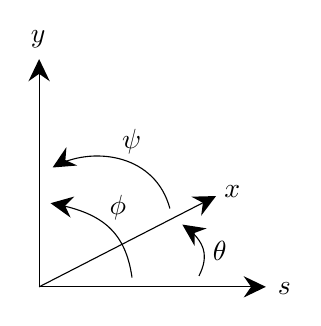
\begin{tikzpicture}[x=0.75pt,y=0.75pt,yscale=-1,xscale=1]
		%uncomment if require: \path (0,232); %set diagram left start at 0, and has height of 232
		
		%Straight Lines [id:da20170232008889133] 
		\draw    (30.75,200.25) -- (30.75,93.5) ;
		\draw [shift={(30.75,90.5)}, rotate = 90] [fill={rgb, 255:red, 0; green, 0; blue, 0 }  ][line width=0.08]  [draw opacity=0] (10.72,-5.15) -- (0,0) -- (10.72,5.15) -- (7.12,0) -- cycle    ;
		%Straight Lines [id:da7586738429193832] 
		\draw    (30.75,200.25) -- (137,200.25) ;
		\draw [shift={(140,200.25)}, rotate = 180] [fill={rgb, 255:red, 0; green, 0; blue, 0 }  ][line width=0.08]  [draw opacity=0] (10.72,-5.15) -- (0,0) -- (10.72,5.15) -- (7.12,0) -- cycle    ;
		%Straight Lines [id:da8289354712219019] 
		\draw    (30.75,200.25) -- (113.33,157.87) ;
		\draw [shift={(116,156.5)}, rotate = 152.83] [fill={rgb, 255:red, 0; green, 0; blue, 0 }  ][line width=0.08]  [draw opacity=0] (10.72,-5.15) -- (0,0) -- (10.72,5.15) -- (7.12,0) -- cycle    ;
		%Curve Lines [id:da8619095365842171] 
		\draw    (107.75,195) .. controls (111.49,187.52) and (112.39,180.04) .. (102.07,171.95) ;
		\draw [shift={(99.75,170.25)}, rotate = 34.46] [fill={rgb, 255:red, 0; green, 0; blue, 0 }  ][line width=0.08]  [draw opacity=0] (10.72,-5.15) -- (0,0) -- (10.72,5.15) -- (7.12,0) -- cycle    ;
		%Curve Lines [id:da14562765286410684] 
		\draw    (93.75,162.5) .. controls (86.83,136.71) and (58.01,132.59) .. (39.76,141.42) ;
		\draw [shift={(37.25,142.75)}, rotate = 329.74] [fill={rgb, 255:red, 0; green, 0; blue, 0 }  ][line width=0.08]  [draw opacity=0] (10.72,-5.15) -- (0,0) -- (10.72,5.15) -- (7.12,0) -- cycle    ;
		%Curve Lines [id:da5921182448586806] 
		\draw    (75.5,195.75) .. controls (72.38,173.67) and (61.01,164.86) .. (39.05,160.48) ;
		\draw [shift={(36.25,159.95)}, rotate = 10.01] [fill={rgb, 255:red, 0; green, 0; blue, 0 }  ][line width=0.08]  [draw opacity=0] (10.72,-5.15) -- (0,0) -- (10.72,5.15) -- (7.12,0) -- cycle    ;
		
		% Text Node
		\draw (113.25,177.15) node [anchor=north west][inner sep=0.75pt]    {$\theta $};
		% Text Node
		\draw (25.5,75.65) node [anchor=north west][inner sep=0.75pt]    {$y$};
		% Text Node
		\draw (118.75,150.15) node [anchor=north west][inner sep=0.75pt]    {$x$};
		% Text Node
		\draw (144.5,197.15) node [anchor=north west][inner sep=0.75pt]    {$s$};
		% Text Node
		\draw (69.5,123.19) node [anchor=north west][inner sep=0.75pt]    {$\psi $};
		% Text Node
		\draw (63.48,154.9) node [anchor=north west][inner sep=0.75pt]    {$\phi $};
	\end{tikzpicture}
	\caption{MAD-like coordinate system}\label{fig:mad-like-coordinates}
\end{figure}

For our calculations, we will represent the reference frame transformations using $4 \times 4$ augmented matrices.
We shall assume the following notation convention: each matrix $M$ consists of entries from $M_{00}$ (top left corner), through $M_{03}$ (top right corner), to $M_{33}$ (bottom right corner).
In particular, we distinguish 4 basic transformations:

\[
	\mathrm{T}(x, y, s) := \begin{bmatrix}
		1 & 0 & 0 & x \\
		0 & 1 & 0 & y \\
		0 & 0 & 1 & s \\
		0 & 0 & 0 & 1
	\end{bmatrix} \;\;\text{(translation)}
\]

\[
	\mathrm{R}_x(\phi) := \begin{bmatrix}
		1 & 0 & 0 & 0 \\
		0 & \cos(\phi) & \sin(\phi) & 0 \\
		0 & -\sin(\phi) & \cos(\phi) & 0 \\
		0 & 0 & 0 & 1
	\end{bmatrix} \;\;\text{(rotation around the $x$ axis)}
\]

\[
	\mathrm{R}_y(\theta) := \begin{bmatrix}
		\cos(\theta) & 0 & \sin(\theta) & 0 \\
		0 & 1 & 0 & 0 \\
		-\sin(\theta) & 0 & \cos(\theta) & 0 \\
		0 & 0 & 0 & 1
	\end{bmatrix} \;\;\text{(rotation around the $y$ axis)}
\]

\[
	\mathrm{R}_s(\psi) := \begin{bmatrix}
		\cos(\psi) & -\sin(\psi) & 0 & 0 \\
		\sin(\psi) & \cos(\psi) & 0 & 0 \\
		0 & 0 & 1 & 0 \\
		0 & 0 & 0 & 1
	\end{bmatrix} \;\;\text{(rotation around the $s$ axis)}
\]
We allow the notation $T_x(\Delta x)$ to mean $T(\Delta x, 0, 0)$, and so on, for $T_y(\Delta y)$ and $T_s(\Delta s)$.


\section{Misalignment at arbitrary $s$ without a tilt}\label{section:curved-no-roll}

We consider a potentially curved element misaligned with respect to an arbitrary position along its length.

\begin{figure}[H]
	\centering
	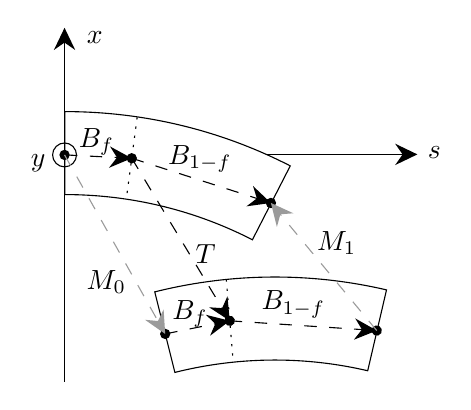
\begin{tikzpicture}[x=0.75pt,y=0.75pt,yscale=-1,xscale=1]
		%uncomment if require: \path (0,300); %set diagram left start at 0, and has height of 300
		
		%Straight Lines [id:da797458358196216] 
		\draw    (121.25,70.82) -- (191.11,70.82) ;
		\draw [shift={(194.11,70.82)}, rotate = 180] [fill={rgb, 255:red, 0; green, 0; blue, 0 }  ][line width=0.08]  [draw opacity=0] (10.72,-5.15) -- (0,0) -- (10.72,5.15) -- (7.12,0) -- cycle    ;
		%Straight Lines [id:da5268015128426032] 
		\draw    (24.11,180.32) -- (24.11,12.82) ;
		\draw [shift={(24.11,9.82)}, rotate = 90] [fill={rgb, 255:red, 0; green, 0; blue, 0 }  ][line width=0.08]  [draw opacity=0] (10.72,-5.15) -- (0,0) -- (10.72,5.15) -- (7.12,0) -- cycle    ;
		%Shape: Ellipse [id:dp6042944787247156] 
		\draw   (20.02,75.11) .. controls (17.78,72.86) and (17.8,69.22) .. (20.06,66.98) .. controls (22.32,64.75) and (25.96,64.77) .. (28.19,67.02) .. controls (30.43,69.28) and (30.41,72.92) .. (28.15,75.16) .. controls (25.89,77.39) and (22.25,77.37) .. (20.02,75.11) -- cycle ;
		%Flowchart: Connector [id:dp3071692594828601] 
		\draw  [draw opacity=0][fill={rgb, 255:red, 0; green, 0; blue, 0 }  ,fill opacity=1 ] (21.61,71.07) .. controls (21.61,69.69) and (22.72,68.57) .. (24.11,68.57) .. controls (25.49,68.57) and (26.61,69.69) .. (26.61,71.07) .. controls (26.61,72.45) and (25.49,73.57) .. (24.11,73.57) .. controls (22.72,73.57) and (21.61,72.45) .. (21.61,71.07) -- cycle ;
		
		%Shape: Block Arc [id:dp07942148731975829] 
		\draw   (24.3,50.19) .. controls (24.5,50.19) and (24.69,50.19) .. (24.89,50.2) .. controls (63.78,50.3) and (100.48,59.73) .. (132.86,76.36) -- (114.62,111.95) .. controls (87.67,98.12) and (57.14,90.27) .. (24.77,90.18) .. controls (24.61,90.18) and (24.45,90.18) .. (24.29,90.18) -- cycle ;
		%Flowchart: Connector [id:dp3735648309295102] 
		\draw  [draw opacity=0][fill={rgb, 255:red, 0; green, 0; blue, 0 }  ,fill opacity=1 ] (121.04,94.28) .. controls (121.01,92.9) and (122.1,91.75) .. (123.48,91.72) .. controls (124.86,91.69) and (126.01,92.78) .. (126.04,94.16) .. controls (126.07,95.54) and (124.98,96.69) .. (123.6,96.72) .. controls (122.22,96.75) and (121.07,95.66) .. (121.04,94.28) -- cycle ;
		%Straight Lines [id:da2366039478899269] 
		\draw  [dash pattern={on 4.5pt off 4.5pt}]  (24.28,71.06) -- (53.48,72.52) ;
		\draw [shift={(56.48,72.67)}, rotate = 182.86] [fill={rgb, 255:red, 0; green, 0; blue, 0 }  ][line width=0.08]  [draw opacity=0] (10.72,-5.15) -- (0,0) -- (10.72,5.15) -- (7.12,0) -- cycle    ;
		%Flowchart: Connector [id:dp8051968426783745] 
		\draw  [draw opacity=0][fill={rgb, 255:red, 0; green, 0; blue, 0 }  ,fill opacity=1 ] (53.98,72.73) .. controls (53.95,71.35) and (55.04,70.21) .. (56.42,70.18) .. controls (57.8,70.14) and (58.95,71.24) .. (58.98,72.62) .. controls (59.01,74) and (57.92,75.14) .. (56.54,75.17) .. controls (55.16,75.21) and (54.01,74.11) .. (53.98,72.73) -- cycle ;
		%Straight Lines [id:da5904317932248363] 
		\draw  [dash pattern={on 4.5pt off 4.5pt}]  (56.48,72.67) -- (120.68,93.3) ;
		\draw [shift={(123.54,94.22)}, rotate = 197.81] [fill={rgb, 255:red, 0; green, 0; blue, 0 }  ][line width=0.08]  [draw opacity=0] (10.72,-5.15) -- (0,0) -- (10.72,5.15) -- (7.12,0) -- cycle    ;
		%Shape: Block Arc [id:dp3422197187906486] 
		\draw   (67.57,137.06) .. controls (67.76,137.01) and (67.94,136.96) .. (68.13,136.92) .. controls (105.89,127.58) and (143.78,127.83) .. (179.23,136.1) -- (170.17,175.06) .. controls (140.67,168.17) and (109.15,167.97) .. (77.73,175.74) .. controls (77.57,175.77) and (77.41,175.81) .. (77.26,175.85) -- cycle ;
		%Flowchart: Connector [id:dp3058023403472935] 
		\draw  [draw opacity=0][fill={rgb, 255:red, 0; green, 0; blue, 0 }  ,fill opacity=1 ] (172.11,156.36) .. controls (171.74,155.03) and (172.53,153.65) .. (173.86,153.28) .. controls (175.19,152.92) and (176.56,153.7) .. (176.93,155.03) .. controls (177.3,156.36) and (176.51,157.74) .. (175.18,158.11) .. controls (173.85,158.47) and (172.48,157.69) .. (172.11,156.36) -- cycle ;
		%Straight Lines [id:da06890321170988856] 
		\draw  [dash pattern={on 4.5pt off 4.5pt}]  (72.6,157.31) -- (100.77,151.6) ;
		\draw [shift={(103.71,151)}, rotate = 168.53] [fill={rgb, 255:red, 0; green, 0; blue, 0 }  ][line width=0.08]  [draw opacity=0] (10.72,-5.15) -- (0,0) -- (10.72,5.15) -- (7.12,0) -- cycle    ;
		%Flowchart: Connector [id:dp2878241642690408] 
		\draw  [draw opacity=0][fill={rgb, 255:red, 0; green, 0; blue, 0 }  ,fill opacity=1 ] (101.3,151.66) .. controls (100.93,150.33) and (101.71,148.96) .. (103.04,148.59) .. controls (104.38,148.22) and (105.75,149.01) .. (106.12,150.34) .. controls (106.48,151.67) and (105.7,153.05) .. (104.37,153.41) .. controls (103.04,153.78) and (101.66,153) .. (101.3,151.66) -- cycle ;
		%Straight Lines [id:da3521010885853867] 
		\draw  [dash pattern={on 4.5pt off 4.5pt}]  (103.71,151) -- (171.53,155.5) ;
		\draw [shift={(174.52,155.69)}, rotate = 183.79] [fill={rgb, 255:red, 0; green, 0; blue, 0 }  ][line width=0.08]  [draw opacity=0] (10.72,-5.15) -- (0,0) -- (10.72,5.15) -- (7.12,0) -- cycle    ;
		%Flowchart: Connector [id:dp35613516370993914] 
		\draw  [draw opacity=0][fill={rgb, 255:red, 0; green, 0; blue, 0 }  ,fill opacity=1 ] (70.1,157.37) .. controls (70.07,155.99) and (71.17,154.84) .. (72.55,154.81) .. controls (73.93,154.78) and (75.07,155.87) .. (75.1,157.25) .. controls (75.14,158.63) and (74.04,159.78) .. (72.66,159.81) .. controls (71.28,159.84) and (70.14,158.75) .. (70.1,157.37) -- cycle ;
		%Straight Lines [id:da881388803539509] 
		\draw  [dash pattern={on 4.5pt off 4.5pt}]  (56.48,72.67) -- (102.16,148.43) ;
		\draw [shift={(103.71,151)}, rotate = 238.91] [fill={rgb, 255:red, 0; green, 0; blue, 0 }  ][line width=0.08]  [draw opacity=0] (10.72,-5.15) -- (0,0) -- (10.72,5.15) -- (7.12,0) -- cycle    ;
		%Straight Lines [id:da07326003199202691] 
		\draw [color={rgb, 255:red, 155; green, 155; blue, 155 }  ,draw opacity=1 ] [dash pattern={on 4.5pt off 4.5pt}]  (24.11,71.07) -- (71.13,154.7) ;
		\draw [shift={(72.6,157.31)}, rotate = 240.65] [fill={rgb, 255:red, 155; green, 155; blue, 155 }  ,fill opacity=1 ][line width=0.08]  [draw opacity=0] (10.72,-5.15) -- (0,0) -- (10.72,5.15) -- (7.12,0) -- cycle    ;
		%Straight Lines [id:da5449253722191645] 
		\draw [color={rgb, 255:red, 155; green, 155; blue, 155 }  ,draw opacity=1 ] [dash pattern={on 4.5pt off 4.5pt}]  (174.52,155.69) -- (125.45,96.53) ;
		\draw [shift={(123.54,94.22)}, rotate = 50.33] [fill={rgb, 255:red, 155; green, 155; blue, 155 }  ,fill opacity=1 ][line width=0.08]  [draw opacity=0] (10.72,-5.15) -- (0,0) -- (10.72,5.15) -- (7.12,0) -- cycle    ;
		%Straight Lines [id:da0006877697562143181] 
		\draw  [dash pattern={on 0.84pt off 2.51pt}]  (59.1,52.92) -- (53.85,92.42) ;
		%Straight Lines [id:da06332771626503675] 
		\draw  [dash pattern={on 0.84pt off 2.51pt}]  (102.03,131.04) -- (105.38,170.96) ;
		
		% Text Node
		\draw (33.61,10.47) node [anchor=north west][inner sep=0.75pt]    {$x$};
		% Text Node
		\draw (197.86,65.97) node [anchor=north west][inner sep=0.75pt]    {$s$};
		% Text Node
		\draw (6.61,69.72) node [anchor=north west][inner sep=0.75pt]    {$y$};
		% Text Node
		\draw (29.75,57.15) node [anchor=north west][inner sep=0.75pt]    {$B_{f}$};
		% Text Node
		\draw (72.75,65.4) node [anchor=north west][inner sep=0.75pt]    {$B_{1-f}$};
		% Text Node
		\draw (74.75,140.15) node [anchor=north west][inner sep=0.75pt]    {$B_{f}$};
		% Text Node
		\draw (117.75,135.4) node [anchor=north west][inner sep=0.75pt]    {$B_{1-f}$};
		% Text Node
		\draw (86,112.9) node [anchor=north west][inner sep=0.75pt]    {$T$};
		% Text Node
		\draw (33.5,125.4) node [anchor=north west][inner sep=0.75pt]    {$M_{0}$};
		% Text Node
		\draw (144.5,106.65) node [anchor=north west][inner sep=0.75pt]    {$M_{1}$};
	\end{tikzpicture}
	\caption{Transformations for a curved element misaligned at an arbitrary $s$.}
\end{figure}

Assuming a curved element of length $L$ that bends the reference frame by $\alpha$ (and therefore a radius of curvature $\rho = L / \alpha$), we can represent $B$ as a combination of a translation and a rotation, $B := T(\Delta x, 0, \Delta s) R_y(-\alpha)$, where
\begin{equation}\label{eq:curved-frame-change}
	\begin{aligned}
		\Delta x &= \rho (\cos(\alpha) - 1) = - L \mathrm{sinc}(\alpha / 2) \sin(\alpha / 2), \\
		\Delta s &= \rho \sin(\alpha) = L \mathrm{sinc}(\alpha).
	\end{aligned}
\end{equation}
Note, that the second formulations of $\Delta x$ and $\Delta s$ let us avoid division by zero if $\alpha = 0$, catering also to the case of a straight element for a truly general case.

Let us say that our element is misaligned at position $\Delta L$ along its length $L$.
Then we can decompose our reference-frame-bending transformation $B$ into parts $B_f$ and $B_{1-f}$ so that $B = B_f B_{1-f}$.
The respective bending angles of the two parts are simply $f \alpha$ and $(1 - f) \alpha$, where $f := \Delta L/L = \Delta L / (\rho \alpha)$ and $\rho$ is the curvature.
Knowing these parameters, it is trivial to construct $B_f$ and $B_{1 - f}$ analogously to $B$, as shown in eq.~\ref{eq:curved-frame-change}.

Then, we compute the following transformation, which will take us from the normal to the misaligned element entry frame:
\[
	M_0 = B_f T B_f^{-1},
\]
whereas for returning to the normal frame from the exit
\[
	\begin{aligned}
		B_f T B_{1 - f} M_1 &= B = B_f B_{1-f}, \\
		M_1 &= (T B_{1 - f})^{-1} B_{1-f} = B_{1 - f}^{-1} T^{-1} B_{1-f}.
	\end{aligned}
\]

When evaluated, the matrix for the curved element in the general case is
\[
	B_f := \begin{bmatrix}
		\cos\left(\alpha f\right) & 0 & -\sin\left(\alpha f\right) & \rho (\cos\left(\alpha f\right) - 1) \\
		0 & 1 & 0 & 0 \\
		\sin\left(\alpha f\right) & 0 & \cos\left(\alpha f\right) & \rho \sin(\alpha f) \\
		0 & 0 & 0 & 1
	\end{bmatrix},
\]
and so
\[
	B_f^{-1} := \begin{bmatrix}
			\cos\left(\alpha f\right) & 0 & \sin\left(\alpha f\right) & \rho (\cos\left(\alpha f\right) - 1) \\
		0 & 1 & 0 & 0 \\
		-\sin\left(\alpha f\right) & 0 & \cos\left(\alpha f\right) & - \rho \sin(\alpha f) \\
		0 & 0 & 0 & 1
		\end{bmatrix}.
\]
Note that $B_{f,03} = (B_f^{-1})_{03} = -L f \mathrm{sinc}(\alpha f / 2) \sin(\alpha f / 2)$ and $B_{f,23} = -(B_f^{-1})_{23} = L f \mathrm{sinc}(\alpha f)$.

Meanwhile, the misalignment matrix is (let $s_\phi := \sin(\phi)$, $c_\psi := \cos(\psi)$, etc., for space-saving reasons)
\[
	T = \begin{bmatrix}
		-s_\phi s_\psi s_\theta + c_\psi c_\theta & -c_\psi s_\phi s_\theta - c_\theta s_\psi & c_\phi s_\theta & x \\
		c_\phi s_\psi & c_\phi c_\psi & s_\phi & y \\
		-c_\theta s_\phi s_\psi - c_\psi s_\theta & -c_\psi c_\theta s_\phi + s_\psi s_\theta & c_\phi c_\theta & s \\
		0 & 0 & 0 & 1
	\end{bmatrix}
\]
and its inverse, since $T$ is a rigid affine transformation, can be computed with
\[
	T^{-1} = \begin{bmatrix}
			R^T & -R^T t \\
			0 & 1
		\end{bmatrix}, \text{ given } \begin{bmatrix}
			R & t \\
			0 & 1
		\end{bmatrix} := T.
\]
%which expands into the matrix
%\[
%	\begin{bmatrix}
%		-s_\phi s_\psi s_\theta + c_\psi c_\theta & c_\phi s_\psi & -c_\theta s_\phi s_\psi - c_\psi s_\theta & (s_\phi s_\psi s - c_\psi x) c_\theta + (s_\phi s_\psi x + c_\psi s) s_\theta - c_\phi s_\psi y \\
%		-c_\psi s_\phi s_\theta - c_\theta s_\psi & c_\phi c_\psi & -c_\psi c_\theta s_\phi + s_\psi s_\theta & (c_\psi s_\phi s + s_\psi x) c_\theta + (c_\psi s_\phi x - s_\psi s) s_\theta - c_\phi c_\psi y \\
%		c_\phi s_\theta & s_\phi & c_\phi c_\theta & -c_\phi c_\theta s - c_\phi s_\theta x - s_\phi y \\
%		0 & 0 & 0 & 1
%	\end{bmatrix}.
%\]

For the conversion from $M_0$ and $M_1$ to the basic tracking transformations, we can use the decomposition, $M_0 = T(x_0, y_0, s_0) R_y(\theta_0) R_x(\phi_0) R_s(\psi_0)$, for which the parameters are as follows
\[
	\begin{aligned}
		\theta_0 &= \arctan_2(M_{0,02}, M_{0,22}), \\
		\phi_0 &= \arctan_2(M_{0,12}, \sqrt{M_{0,10}^2 + M_{0,11}^2}), \\
		\psi_0 &= \arctan_2(M_{0,10}, M_{0,11}), \\
		x_0 &= M_{0,03}, \\
		y_0 &= M_{0,13}, \\
		s_0 &= M_{0,23},
	\end{aligned}
\]
and for the exit, $M_1 = T(x_1, y_1, s_1) R_y(\theta_1) R_x(\phi_1) R_s(\psi_1)$,
\[
	\begin{aligned}
		\theta_1 &= \arctan_2(M_{1,02}, M_{1,22}), \\
		\phi_1 &= \arctan_2(M_{1,12}, \sqrt{M_{1,10}^2 + M_{1,11}^2}), \\
		\psi_1 &= \arctan_2(M_{1,10}, M_{1,11}), \\
		x_1 &= M_{1,03}, \\
		y_1 &= M_{1,13}, \\
		s_1 &= M_{1,23}.
	\end{aligned}
\]
Note that many decompositions are possible, and their order can lead to more or less clean closed formulae for the parameters; in this case, however, we do not expect any `nice' closed-form solutions (as opposed to the case of the subsequent section!)
The above decomposition corresponds to the following tracking sequence:
\begin{itemize}
	\item ($M_0$:) XYShift($x_0$, $y_0$), SShift($s_0$), YRot($\theta_0$), XRot($\phi_0$), SRot($\psi_0$),
	\item ($B$:) Element($L$, $\alpha$),
	\item ($M_1$:) XYShift($x_1$, $y_1$), SShift($s_1$), YRot($\theta_1$), XRot($\phi_1$), SRot($\psi_1$).
\end{itemize}


\section{Misalignment at arbitrary $s$ (the straight case)}\label{section:straight}

Analogously to the previous section, we split $D$ into $D_f D_{1-f}$:
\begin{figure}[H]
	\centering
	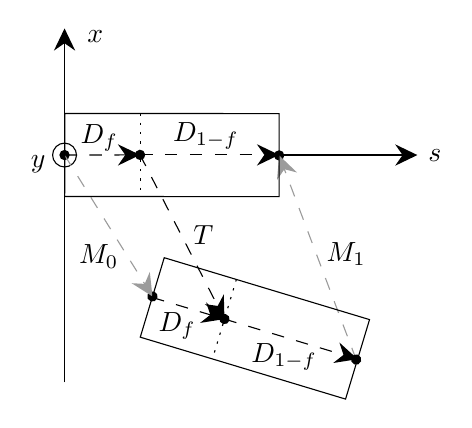
\begin{tikzpicture}[x=0.75pt,y=0.75pt,yscale=-1,xscale=1]
		%uncomment if require: \path (0,300); %set diagram left start at 0, and has height of 300
		
		%Straight Lines [id:da35507818785418455] 
		\draw    (127.5,70.82) -- (191.11,70.82) ;
		\draw [shift={(194.11,70.82)}, rotate = 180] [fill={rgb, 255:red, 0; green, 0; blue, 0 }  ][line width=0.08]  [draw opacity=0] (10.72,-5.15) -- (0,0) -- (10.72,5.15) -- (7.12,0) -- cycle    ;
		%Straight Lines [id:da8526813980418886] 
		\draw    (24.11,180.32) -- (24.11,12.82) ;
		\draw [shift={(24.11,9.82)}, rotate = 90] [fill={rgb, 255:red, 0; green, 0; blue, 0 }  ][line width=0.08]  [draw opacity=0] (10.72,-5.15) -- (0,0) -- (10.72,5.15) -- (7.12,0) -- cycle    ;
		%Flowchart: Connector [id:dp5359668052415314] 
		\draw  [draw opacity=0][fill={rgb, 255:red, 0; green, 0; blue, 0 }  ,fill opacity=1 ] (125,71) .. controls (125,69.62) and (126.12,68.5) .. (127.5,68.5) .. controls (128.88,68.5) and (130,69.62) .. (130,71) .. controls (130,72.38) and (128.88,73.5) .. (127.5,73.5) .. controls (126.12,73.5) and (125,72.38) .. (125,71) -- cycle ;
		%Straight Lines [id:da6177744279918915] 
		\draw [color={rgb, 255:red, 155; green, 155; blue, 155 }  ,draw opacity=1 ] [dash pattern={on 4.5pt off 4.5pt}]  (164.61,169.34) -- (128.56,73.81) ;
		\draw [shift={(127.5,71)}, rotate = 69.32] [fill={rgb, 255:red, 155; green, 155; blue, 155 }  ,fill opacity=1 ][line width=0.08]  [draw opacity=0] (10.72,-5.15) -- (0,0) -- (10.72,5.15) -- (7.12,0) -- cycle    ;
		%Flowchart: Connector [id:dp7969702218848098] 
		\draw  [draw opacity=0][fill={rgb, 255:red, 0; green, 0; blue, 0 }  ,fill opacity=1 ] (64.14,138.06) .. controls (64.63,136.77) and (66.07,136.12) .. (67.36,136.62) .. controls (68.65,137.11) and (69.3,138.55) .. (68.81,139.84) .. controls (68.32,141.13) and (66.87,141.78) .. (65.58,141.29) .. controls (64.29,140.8) and (63.65,139.35) .. (64.14,138.06) -- cycle ;
		%Flowchart: Connector [id:dp09475937969231463] 
		\draw  [draw opacity=0][fill={rgb, 255:red, 0; green, 0; blue, 0 }  ,fill opacity=1 ] (162.27,168.45) .. controls (162.77,167.16) and (164.21,166.51) .. (165.5,167) .. controls (166.79,167.49) and (167.44,168.94) .. (166.95,170.23) .. controls (166.45,171.52) and (165.01,172.16) .. (163.72,171.67) .. controls (162.43,171.18) and (161.78,169.74) .. (162.27,168.45) -- cycle ;
		%Shape: Ellipse [id:dp5244406786344289] 
		\draw   (20.02,74.86) .. controls (17.78,72.61) and (17.8,68.97) .. (20.06,66.73) .. controls (22.32,64.5) and (25.96,64.52) .. (28.19,66.77) .. controls (30.43,69.03) and (30.41,72.67) .. (28.15,74.91) .. controls (25.89,77.14) and (22.25,77.12) .. (20.02,74.86) -- cycle ;
		%Flowchart: Connector [id:dp7900569932281408] 
		\draw  [draw opacity=0][fill={rgb, 255:red, 0; green, 0; blue, 0 }  ,fill opacity=1 ] (21.61,70.82) .. controls (21.61,69.44) and (22.72,68.32) .. (24.11,68.32) .. controls (25.49,68.32) and (26.61,69.44) .. (26.61,70.82) .. controls (26.61,72.2) and (25.49,73.32) .. (24.11,73.32) .. controls (22.72,73.32) and (21.61,72.2) .. (21.61,70.82) -- cycle ;
		
		%Straight Lines [id:da20442801210117567] 
		\draw [color={rgb, 255:red, 155; green, 155; blue, 155 }  ,draw opacity=1 ] [dash pattern={on 4.5pt off 4.5pt}]  (24.11,70.82) -- (64.89,136.4) ;
		\draw [shift={(66.47,138.95)}, rotate = 238.12] [fill={rgb, 255:red, 155; green, 155; blue, 155 }  ,fill opacity=1 ][line width=0.08]  [draw opacity=0] (10.72,-5.15) -- (0,0) -- (10.72,5.15) -- (7.12,0) -- cycle    ;
		%Straight Lines [id:da774139029064869] 
		\draw  [dash pattern={on 4.5pt off 4.5pt}]  (24.11,70.82) -- (57.5,70.76) ;
		\draw [shift={(60.5,70.75)}, rotate = 179.89] [fill={rgb, 255:red, 0; green, 0; blue, 0 }  ][line width=0.08]  [draw opacity=0] (10.72,-5.15) -- (0,0) -- (10.72,5.15) -- (7.12,0) -- cycle    ;
		%Flowchart: Connector [id:dp1702286240852332] 
		\draw  [draw opacity=0][fill={rgb, 255:red, 0; green, 0; blue, 0 }  ,fill opacity=1 ] (58.01,70.93) .. controls (57.91,69.55) and (58.94,68.36) .. (60.32,68.26) .. controls (61.7,68.16) and (62.89,69.19) .. (62.99,70.57) .. controls (63.09,71.95) and (62.06,73.14) .. (60.68,73.24) .. controls (59.3,73.34) and (58.11,72.31) .. (58.01,70.93) -- cycle ;
		%Straight Lines [id:da6390869763810431] 
		\draw  [dash pattern={on 4.5pt off 4.5pt}]  (60.5,70.75) -- (124.5,70.75) ;
		\draw [shift={(127.5,70.75)}, rotate = 180] [fill={rgb, 255:red, 0; green, 0; blue, 0 }  ][line width=0.08]  [draw opacity=0] (10.72,-5.15) -- (0,0) -- (10.72,5.15) -- (7.12,0) -- cycle    ;
		%Shape: Rectangle [id:dp5029720108971986] 
		\draw   (24.19,50.8) -- (127.5,50.84) -- (127.49,90.84) -- (24.18,90.8) -- cycle ;
		%Straight Lines [id:da5919731693823477] 
		\draw  [dash pattern={on 0.84pt off 2.51pt}]  (60.5,50.75) -- (60.5,90.75) ;
		%Straight Lines [id:da7746066807011568] 
		\draw  [dash pattern={on 4.5pt off 4.5pt}]  (66.29,139.41) -- (98.28,148.98) ;
		\draw [shift={(101.15,149.84)}, rotate = 196.65] [fill={rgb, 255:red, 0; green, 0; blue, 0 }  ][line width=0.08]  [draw opacity=0] (10.72,-5.15) -- (0,0) -- (10.72,5.15) -- (7.12,0) -- cycle    ;
		%Flowchart: Connector [id:dp7156618154401919] 
		\draw  [draw opacity=0][fill={rgb, 255:red, 0; green, 0; blue, 0 }  ,fill opacity=1 ] (98.71,149.3) .. controls (99.02,147.95) and (100.35,147.1) .. (101.7,147.4) .. controls (103.05,147.7) and (103.9,149.04) .. (103.59,150.39) .. controls (103.29,151.74) and (101.96,152.58) .. (100.61,152.28) .. controls (99.26,151.98) and (98.41,150.65) .. (98.71,149.3) -- cycle ;
		%Straight Lines [id:da69262585053882] 
		\draw  [dash pattern={on 4.5pt off 4.5pt}]  (101.15,149.84) -- (162.44,168.3) ;
		\draw [shift={(165.31,169.16)}, rotate = 196.76] [fill={rgb, 255:red, 0; green, 0; blue, 0 }  ][line width=0.08]  [draw opacity=0] (10.72,-5.15) -- (0,0) -- (10.72,5.15) -- (7.12,0) -- cycle    ;
		%Shape: Rectangle [id:dp06216288058859021] 
		\draw   (72.14,120.28) -- (171.05,150.1) -- (159.5,188.4) -- (60.59,158.57) -- cycle ;
		%Straight Lines [id:da15643091065704995] 
		\draw  [dash pattern={on 0.84pt off 2.51pt}]  (106.92,130.69) -- (95.39,168.99) ;
		%Straight Lines [id:da3239479052474509] 
		\draw  [dash pattern={on 4.5pt off 4.5pt}]  (60.5,70.75) -- (99.78,147.18) ;
		\draw [shift={(101.15,149.84)}, rotate = 242.8] [fill={rgb, 255:red, 0; green, 0; blue, 0 }  ][line width=0.08]  [draw opacity=0] (10.72,-5.15) -- (0,0) -- (10.72,5.15) -- (7.12,0) -- cycle    ;
		
		% Text Node
		\draw (33.86,9.72) node [anchor=north west][inner sep=0.75pt]    {$x$};
		% Text Node
		\draw (198.11,66.72) node [anchor=north west][inner sep=0.75pt]    {$s$};
		% Text Node
		\draw (29.86,112.89) node [anchor=north west][inner sep=0.75pt]    {$M_{0}$};
		% Text Node
		\draw (149.11,111.72) node [anchor=north west][inner sep=0.75pt]    {$M_{1}$};
		% Text Node
		\draw (6.61,69.72) node [anchor=north west][inner sep=0.75pt]    {$y$};
		% Text Node
		\draw (84.86,103.47) node [anchor=north west][inner sep=0.75pt]    {$T$};
		% Text Node
		\draw (30.61,54.72) node [anchor=north west][inner sep=0.75pt]    {$D_{f}$};
		% Text Node
		\draw (68.11,145.22) node [anchor=north west][inner sep=0.75pt]    {$D_{f}$};
		% Text Node
		\draw (75.11,53.97) node [anchor=north west][inner sep=0.75pt]    {$D_{1-f}$};
		% Text Node
		\draw (112.86,160.22) node [anchor=north west][inner sep=0.75pt]    {$D_{1-f}$};
	\end{tikzpicture}
	\caption{A straight element misaligned at an arbitrary location.}
\end{figure}

We simply have that $D_f := T(0, 0, fL)$ and $D_{1-f} := T(0, 0, (1-f)L)$.
To get to the misaligned entry frame we have
\[
	M_0 := D_f T D_f^{-1} = T_s(fL) \; T \; T_s(-fL),
\]
whereas for returning to the normal frame from the exit
\[
	\begin{aligned}
		M_1 := D_{1-f}^{-1} T^{-1} D_{1-f} = T_s((f-1)L) \; T^{-1} \; T_s((1-f)L).
	\end{aligned}
\]

It is intuitively obvious, that due to lack of curvature, the entry and exit transformations should be possible to simplify.
Specifically, we would want $M_0$ to involve some translation followed by rotations $R_y(\theta) R_x(\phi) R_s(\psi)$, and $M_1$, since it `undoes' the effect of $M_0$, into rotations $R_s(-\psi) R_x(-\phi) R_y(-\theta)$ followed by some other translation.

First we decompose the entry matrix $M_0 = T(x_0, y_0, s_0) R_y(\theta_0) R_x(\phi_0) R_s(\psi_0)$, i.e.~with the same method as in the previous section.
After some algebra we observe that the angles and shifts indeed simplify:
\[
	\begin{aligned}
		\theta_0 &= \arctan_2(M_{0,02}, M_{0,22}) = \theta, \\
		\phi_0 &= \arctan_2(M_{0,12}, \sqrt{M_{0,10}^2 + M_{0,11}^2}) = \phi, \\
		\psi_0 &= \arctan_2(M_{0,10}, M_{0,11}) = \psi, \\
		x_0 &= T_{0,03} = x - L f \cos(\phi)\sin(\theta), \\
		y_0 &= T_{0,13} = y - L f \sin(\phi), \\
		s_0 &= T_{0,23} = s - L f (\cos(\phi)\cos(\theta) - 1).
	\end{aligned}
\]

Let us now decompose the matrix $M_1$ into $R_s(\psi_1) R_x(\phi_1) R_y(\theta_1) T(x_1, y_1, s_1)$.
To this end, let us write separately as $M_{rot}$ and $M_{tr}$ the rotation and translation part of the above decomposition, i.e.~let $M_{rot} = R_s(\psi_1) R_x(\phi_1) R_y(\theta_1)$ and let $M_{tr} := T(x_1, y_1, s_1)$.
In such a decomposition, the rotation part of $M_{rot}$ is the same as that of $M_1$, and so we can simply extract it from there.
Afterwards, knowing $M_{rot}$ we can compute $M_{tr} = M_{rot}^{-1} M_1$ to get the shifts.
We indeed observe the angles and shifts simplifying:
\[
	\begin{aligned}
		\theta_1 &= -\arctan_2(M_{1,20}, M_{1,22}) = -\theta, \\
		\phi_1 &= -\arctan_2(M_{1,21}, \sqrt{M_{1,01}^2 + M_{1,11}^2}) = -\phi, \\
		\psi_1 &= \arctan_2(M_{1,01}, M_{1,11}) = -\psi, \\
		x_1 &= M_{tr,03} = (f - 1) L \cos(\phi) \sin(\theta) - x, \\
		y_1 &= M_{tr,13} = (f - 1) L \sin(\phi) - y, \\
		s_1 &= M_{tr,23} = (f - 1) L (\cos(\phi) \cos(\theta) - 1) - s.
	\end{aligned}
\]
This way, our tracking procedure can be significantly less computationally expensive, compare to that of the preceding section, as no matrix operations are required:
	\begin{itemize}
	\item XYShift($x - L f \cos(\phi)\sin(\theta)$, $y - L f \sin(\phi)$)
	\item SShift($s - L f (1 - \cos(\phi)\cos(\theta))$)
	\item YRot($\theta$), XRot($\phi$), SRot($\psi$),
	\item Element($L$),
	\item SRot($-\psi$), XRot($-\phi$), YRot($-\theta$),
	\item SShift($(f - 1) L (\cos(\phi) \cos(\theta) - 1) - s$),
	\item XYShift($(f - 1) L \cos(\phi) \sin(\theta) - x$, $(f - 1) L \sin(\phi) - y$).
\end{itemize}


\section{Misalignment at arbitrary $s$ with a tilt}

We consider a tilted curved element misaligned with respect to an arbitrary position along its length.

\begin{figure}[H]
	\centering
	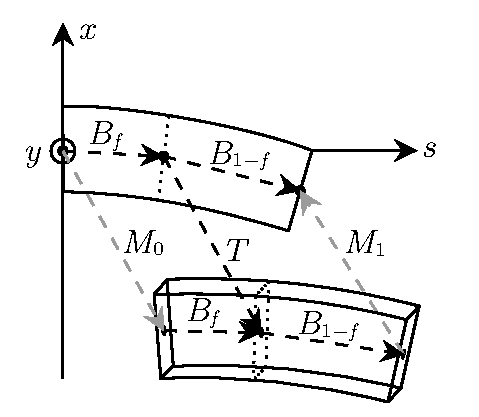
\includegraphics[scale=0.75]{figures/bend-roll.pdf}
	\caption{A tilted curved element misaligned at an arbitrary location.}
	\label{fig:bend-roll}
\end{figure}

Compared with the earlier discussion of misaligned curved elements (see Section~\ref{section:curved-no-roll}), when considering a tilted element, we need to include the tilting in our transformation $B$ (which, as before, is decomposed as $B_f B_{1-f}$ in Figure~\ref{fig:bend-roll}).

In order to include this effect we need to realise that in the previous case the curvature of the reference frame was only applied in the $s{-}x$ plane, whereas in the case of Figure~\ref{fig:bend-roll}, it will be applied in the plane obtained by tilting $s{-}x$ by some angle $\kappa$.

Therefore, taking $B_{sx}$ as the earlier transformation, i.e.,
\[
	B_{sx} := \begin{bmatrix}
		\cos\left(\alpha\right) & 0 & -\sin\left(\alpha\right) & \rho (\cos\left(\alpha\right) - 1) \\
		0 & 1 & 0 & 0 \\
		\sin\left(\alpha\right) & 0 & \cos\left(\alpha\right) & \rho \sin(\alpha) \\
		0 & 0 & 0 & 1
	\end{bmatrix},
\]
and taking $s_\alpha = \sin(\alpha)$, $c_\alpha = \cos(\alpha)$, etc.~for space-saving reasons, we can express $B$ as $R_s(\kappa) \; B_{sx} \; R_s(-\kappa)$, which evaluates to
\[
	B := \begin{bmatrix}
		{\left(c_\alpha - 1\right)} c_\kappa^{2} + 1 & {\left(c_\alpha - 1\right)} c_\kappa s_\kappa & -c_\kappa s_\alpha & \rho {\left(c_\alpha - 1\right)} c_\kappa \\
		{\left(c_\alpha - 1\right)} c_\kappa s_\kappa & {\left(c_\alpha - 1\right)} s_\kappa^{2} + 1 & -s_\alpha s_\kappa & \rho {\left(c_\alpha - 1\right)} s_\kappa \\
		c_\kappa s_\alpha & s_\alpha s_\kappa & c_\alpha & \rho s_\alpha \\
		0 & 0 & 0 & 1
	\end{bmatrix}.
\]
We can obtain the matrices $B_f$ and $B_{1-f}$ by substituting $f \alpha$ and $(1 - f) \alpha$ for $\alpha$ in the above.
To obtain the tracking procedure in this case it suffices to follow the steps of Section~\ref{section:curved-no-roll}, substituting the new matrices.


\section{Misalignment at arbitrary $s$ with a tilt (straight case)}\label{section:straight-roll}

We can generalise the matrix of the above section to a straight case by recalling that $\rho(\cos(\alpha) - 1) = -L \mathrm{sinc}(\alpha / 2) \sin(\alpha / 2)$ and $\rho \sin(\alpha) = L \mathrm{sinc}(\alpha)$.
Then, we can see that when $\alpha = 0$, the matrix $B$ of the preceding section simplifies to
\[
	B \rvert_{\alpha=0} = \begin{bmatrix}
		1 & 0 & 0 & 0 \\
		0 & 1 & 0 & 0 \\
		0 & 0 & 1 & L \\
		0 & 0 & 0 & 1
	\end{bmatrix} = T_s(L) = D.
\]
This means that the effect of the roll is disregarded in the calculation of the reference frame change for the purposes of a misalignment, and, therefore, that we can apply the exact procedure outlined in Section~\ref{section:straight} also for tilted elements.
This makes intuitive sense, as, in our setup, the tilt indeed only affects the direction of curvature of the element: if the element is straight, there is no work to be done for the misalignment, and the element map alone fully describes the effect of the tilt on the particles.


\section{S Shift -- $\zeta$ correction}

In the tracking procedures shown in the preceding sections, we use the tracking map we refer to as an SShift, which we use to transport the particles in a straight line by a displacement in $s$.
We can presume the SShift to be a variant of DriftExact, however there are special considerations that we need to take here, with respect to the path length $s$ and the delay $\zeta$ of our particles.

\begin{figure}[H]
	\centering
	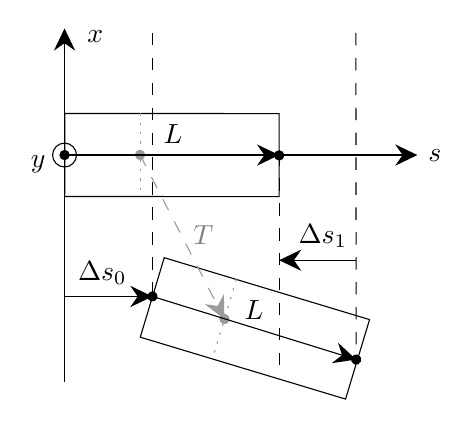
\begin{tikzpicture}[x=0.75pt,y=0.75pt,yscale=-1,xscale=1]
		%Straight Lines [id:da35507818785418455] 
		\draw    (127.75,70.82) -- (191.11,70.82) ;
		\draw [shift={(194.11,70.82)}, rotate = 180] [fill={rgb, 255:red, 0; green, 0; blue, 0 }  ][line width=0.08]  [draw opacity=0] (10.72,-5.15) -- (0,0) -- (10.72,5.15) -- (7.12,0) -- cycle    ;
		%Straight Lines [id:da8526813980418886] 
		\draw    (24.11,180.32) -- (24.11,12.82) ;
		\draw [shift={(24.11,9.82)}, rotate = 90] [fill={rgb, 255:red, 0; green, 0; blue, 0 }  ][line width=0.08]  [draw opacity=0] (10.72,-5.15) -- (0,0) -- (10.72,5.15) -- (7.12,0) -- cycle    ;
		%Flowchart: Connector [id:dp5359668052415314] 
		\draw  [draw opacity=0][fill={rgb, 255:red, 0; green, 0; blue, 0 }  ,fill opacity=1 ] (125,71) .. controls (125,69.62) and (126.12,68.5) .. (127.5,68.5) .. controls (128.88,68.5) and (130,69.62) .. (130,71) .. controls (130,72.38) and (128.88,73.5) .. (127.5,73.5) .. controls (126.12,73.5) and (125,72.38) .. (125,71) -- cycle ;
		%Flowchart: Connector [id:dp7969702218848098] 
		\draw  [draw opacity=0][fill={rgb, 255:red, 0; green, 0; blue, 0 }  ,fill opacity=1 ] (64.14,138.06) .. controls (64.63,136.77) and (66.07,136.12) .. (67.36,136.62) .. controls (68.65,137.11) and (69.3,138.55) .. (68.81,139.84) .. controls (68.32,141.13) and (66.87,141.78) .. (65.58,141.29) .. controls (64.29,140.8) and (63.65,139.35) .. (64.14,138.06) -- cycle ;
		%Flowchart: Connector [id:dp09475937969231463] 
		\draw  [draw opacity=0][fill={rgb, 255:red, 0; green, 0; blue, 0 }  ,fill opacity=1 ] (162.27,168.45) .. controls (162.77,167.16) and (164.21,166.51) .. (165.5,167) .. controls (166.79,167.49) and (167.44,168.94) .. (166.95,170.23) .. controls (166.45,171.52) and (165.01,172.16) .. (163.72,171.67) .. controls (162.43,171.18) and (161.78,169.74) .. (162.27,168.45) -- cycle ;
		%Shape: Ellipse [id:dp5244406786344289] 
		\draw   (20.02,74.86) .. controls (17.78,72.61) and (17.8,68.97) .. (20.06,66.73) .. controls (22.32,64.5) and (25.96,64.52) .. (28.19,66.77) .. controls (30.43,69.03) and (30.41,72.67) .. (28.15,74.91) .. controls (25.89,77.14) and (22.25,77.12) .. (20.02,74.86) -- cycle ;
		%Flowchart: Connector [id:dp7900569932281408] 
		\draw  [draw opacity=0][fill={rgb, 255:red, 0; green, 0; blue, 0 }  ,fill opacity=1 ] (21.61,70.82) .. controls (21.61,69.44) and (22.72,68.32) .. (24.11,68.32) .. controls (25.49,68.32) and (26.61,69.44) .. (26.61,70.82) .. controls (26.61,72.2) and (25.49,73.32) .. (24.11,73.32) .. controls (22.72,73.32) and (21.61,72.2) .. (21.61,70.82) -- cycle ;
		
		%Flowchart: Connector [id:dp1702286240852332] 
		\draw  [draw opacity=0][fill={rgb, 255:red, 155; green, 155; blue, 155 }  ,fill opacity=1 ] (58.01,70.93) .. controls (57.91,69.55) and (58.94,68.36) .. (60.32,68.26) .. controls (61.7,68.16) and (62.89,69.19) .. (62.99,70.57) .. controls (63.09,71.95) and (62.06,73.14) .. (60.68,73.24) .. controls (59.3,73.34) and (58.11,72.31) .. (58.01,70.93) -- cycle ;
		%Shape: Rectangle [id:dp5029720108971986] 
		\draw   (24.19,50.8) -- (127.5,50.84) -- (127.49,90.84) -- (24.18,90.8) -- cycle ;
		%Straight Lines [id:da5919731693823477] 
		\draw [color={rgb, 255:red, 155; green, 155; blue, 155 }  ,draw opacity=1 ] [dash pattern={on 0.84pt off 2.51pt}]  (60.5,50.75) -- (60.5,90.75) ;
		%Flowchart: Connector [id:dp7156618154401919] 
		\draw  [draw opacity=0][fill={rgb, 255:red, 155; green, 155; blue, 155 }  ,fill opacity=1 ] (98.71,149.3) .. controls (99.02,147.95) and (100.35,147.1) .. (101.7,147.4) .. controls (103.05,147.7) and (103.9,149.04) .. (103.59,150.39) .. controls (103.29,151.74) and (101.96,152.58) .. (100.61,152.28) .. controls (99.26,151.98) and (98.41,150.65) .. (98.71,149.3) -- cycle ;
		%Shape: Rectangle [id:dp06216288058859021] 
		\draw   (72.14,120.28) -- (171.05,150.1) -- (159.5,188.4) -- (60.59,158.57) -- cycle ;
		%Straight Lines [id:da15643091065704995] 
		\draw [color={rgb, 255:red, 155; green, 155; blue, 155 }  ,draw opacity=1 ] [dash pattern={on 0.84pt off 2.51pt}]  (106.92,130.69) -- (95.39,168.99) ;
		%Straight Lines [id:da3239479052474509] 
		\draw [color={rgb, 255:red, 155; green, 155; blue, 155 }  ,draw opacity=1 ] [dash pattern={on 4.5pt off 4.5pt}]  (60.5,70.75) -- (99.78,147.18) ;
		\draw [shift={(101.15,149.84)}, rotate = 242.8] [fill={rgb, 255:red, 155; green, 155; blue, 155 }  ,fill opacity=1 ][line width=0.08]  [draw opacity=0] (10.72,-5.15) -- (0,0) -- (10.72,5.15) -- (7.12,0) -- cycle    ;
		%Straight Lines [id:da4836988544272087] 
		\draw  [dash pattern={on 4.5pt off 4.5pt}]  (66.47,12) -- (66.47,138.95) ;
		%Straight Lines [id:da5330246211677179] 
		\draw  [dash pattern={on 4.5pt off 4.5pt}]  (127.5,172) -- (127.5,71) ;
		%Straight Lines [id:da5582054958236305] 
		\draw  [dash pattern={on 4.5pt off 4.5pt}]  (164.47,12) -- (164.61,169.34) ;
		%Straight Lines [id:da2986734039407184] 
		\draw    (23.97,138.95) -- (63.47,138.95) ;
		\draw [shift={(66.47,138.95)}, rotate = 180] [fill={rgb, 255:red, 0; green, 0; blue, 0 }  ][line width=0.08]  [draw opacity=0] (10.72,-5.15) -- (0,0) -- (10.72,5.15) -- (7.12,0) -- cycle    ;
		%Straight Lines [id:da8950058864242387] 
		\draw    (66.47,138.95) -- (161.74,168.45) ;
		\draw [shift={(164.61,169.34)}, rotate = 197.2] [fill={rgb, 255:red, 0; green, 0; blue, 0 }  ][line width=0.08]  [draw opacity=0] (10.72,-5.15) -- (0,0) -- (10.72,5.15) -- (7.12,0) -- cycle    ;
		%Straight Lines [id:da776090670545246] 
		\draw    (164.61,121.5) -- (130.5,121.5) ;
		\draw [shift={(127.5,121.5)}, rotate = 360] [fill={rgb, 255:red, 0; green, 0; blue, 0 }  ][line width=0.08]  [draw opacity=0] (10.72,-5.15) -- (0,0) -- (10.72,5.15) -- (7.12,0) -- cycle    ;
		%Straight Lines [id:da6954530061787899] 
		\draw    (24.11,70.82) -- (124.5,70.82) ;
		\draw [shift={(127.5,70.82)}, rotate = 180] [fill={rgb, 255:red, 0; green, 0; blue, 0 }  ][line width=0.08]  [draw opacity=0] (10.72,-5.15) -- (0,0) -- (10.72,5.15) -- (7.12,0) -- cycle    ;
		
		% Text Node
		\draw (33.86,9.72) node [anchor=north west][inner sep=0.75pt]    {$x$};
		% Text Node
		\draw (198.11,66.72) node [anchor=north west][inner sep=0.75pt]    {$s$};
		% Text Node
		\draw (6.61,69.72) node [anchor=north west][inner sep=0.75pt]    {$y$};
		% Text Node
		\draw (84.86,103.47) node [anchor=north west][inner sep=0.75pt]  {\textcolor{gray}{$T$}};
		% Text Node
		\draw (70.61,54.9) node [anchor=north west][inner sep=0.75pt]    {$L$};
		% Text Node
		\draw (109.61,139.9) node [anchor=north west][inner sep=0.75pt]    {$L$};
		% Text Node
		\draw (29.36,120.9) node [anchor=north west][inner sep=0.75pt]    {$\Delta s_{0}$};
		% Text Node
		\draw (135.61,102.9) node [anchor=north west][inner sep=0.75pt]    {$\Delta s_{1}$};
	\end{tikzpicture}
	\caption{Visualisation of the $s$-coordinate transformations without correction.}\label{fig:no-s-no-zeta-correction}
\end{figure}

In the visualisation in Fig.~\ref{fig:no-s-no-zeta-correction} we can see the different $s$-coordinate updates taking place when we track through a misalignment: in particular, we can see that the total path of the particle travelled, should SShift be simply a drift, is $\Delta s = \Delta s_0 + L + \Delta s_1$.
Clearly, $\Delta s_0 \neq -\Delta s_1$, and so the path length changes between the aligned and misaligned element.
However, what we desire is the opposite, i.e.~that the path length does not change: it is inconvenient to have the length of our accelerator change due to a misalignment.
Therefore, the simplest correction we can make in this instance is to disregard the update of the $s$ coordinate in our drift/$s$-shift.

A further correction needs to be made with respect to the $\zeta$ coordinate.
Since $\zeta$ is related to the path length by $\zeta = s - \beta_0 c t$, and since, in our setup, the synchronous particle arrival time is not expected to change between the normal and misaligned entry to the element we expect that $\Delta \zeta = \Delta s$ between those two points.
However, as we have already established for our correction of $s$, we expect the $s$ coordinate to be unchanged, so we can adjust $\zeta$ in exactly the same fashion as we do $s$:

\[
	\text{SShift}(\Delta s) := ( \text{DriftExact}(\Delta s),\;\; s \leftarrow s - \Delta s,\;\; \zeta \leftarrow \zeta - \Delta s ).
\]


\section{Other notes}

The rotation direction conventions differ between the MAD-X survey coordinate system and the beam coordinate system, in that the $y$-rotation of the beam is opposite to the one described by YRot in the tracking procedures above. This sign difference is taken into account in the Xsuite implementation.